\documentclass[12pt]{article}
\usepackage[left=2.5cm,top=2.0cm,right=2.5cm,bottom=3.0cm]{geometry}
\usepackage[utf8]{inputenc}
\usepackage[english]{babel}
\usepackage{graphicx}
\usepackage{fancyhdr}
\usepackage{url}
\usepackage{xcolor}
\usepackage{multirow}
\usepackage{listings}
\usepackage{float}
\usepackage{subfigure} % subfiguras
\usepackage{csquotes}
\usepackage[backend=bibtex,bibencoding=ascii,style=authoryear,sorting=none]{biblatex}




\usepackage[backend=bibtex]{biblatex}
%\usepackage[backend=biber]{biblatex}
\addbibresource{Bibliografia.bib}





% Actualiza en automático la fecha de las citas de internet a la fecha de la compilación del documento
\usepackage{datetime}
\newdateformat{specialdate}{\twodigit{\THEDAY}-\twodigit{\THEMONTH}-\THEYEAR}
%\newdateformat{specialdate}{\twodigit{\THEDAY}-\THEYEAR}
\date{\specialdate\today}

\newcommand{\HRule}{\rule{\linewidth}{0.25mm}}

% CONSTANTES NECESARIAS PARA EL DOCUMENTO ---> MODIFIQUEN A SU CRITERIO
\newcommand{\matricula}           {0123456789}  %SU MATRICULA
\newcommand{\elola}           {la}  %Hombres cambien LA por EL
\newcommand{\OA}           {a}  %Hombres cambien A por O
\newcommand{\ncuatrimestre}{septiembre-diciembre 2014}
\newcommand{\nproyecto}           {Metodología de automatización y monitoreo a vehículos de gama baja: confort y emisión de gases}
\newcommand{\nproyectoheader}     {Metodología de automatización y monitoreo  \\ a vehículos de gama baja: \\ confort y emisión de gases}
\newcommand{\nalumno}             {ING. BUJANO GUZMÁN GUSTAVO}
\newcommand{\ncarrera}            {MAESTRÍA EN INGENIERÍA }
\newcommand{\nasesorinstitucional}{Dr. MARTÍN HERNÁNDEZ ORDOÑEZ}
\newcommand{\nasesorinstitucionaldos}{Dr. Marco Aurelio Nuño Maganda}

\newcommand{\fecha}               {Diciembre de 2016}
\newcommand{\fechacarta}{1 de Diciembre de 2016}
\newcommand{\separacionCorta}{0.0cm}
\newcommand{\separacionLarga}{0.5cm}

\usepackage[bookmarks=true,bookmarksopen=false,colorlinks=true]{hyperref} % marcadores y propiedades del p 



\usepackage[overload]{textcase}
\newcommand{\iemph}[1]{\MakeTextUppercase{#1}}


\pagestyle{fancy}
\headheight 48pt
\fancyhead{} % Clear all header fields
\fancyhead[L]{
\includegraphics[height=1.5cm]{LogoPOLIS.png}}%
\fancyhead[C]{\nproyectoheader}%
\fancyhead[R]{
\includegraphics[height=1.5cm]{LogoUPV.png}}%
\fancyfoot[R]{Página \thepage} % Clear all footer fields 
\fancyfoot[C]{}
\fancyfoot[L]{}

\DefineBibliographyStrings{english}{%
  references = {Referencias},% replace "references" with "bibliography"  for `book`/`report`
}

\addto\captionsenglish{%
  \renewcommand{\figurename}{Figura}%
  \renewcommand{\tablename}{Cuadro}%
} 
 
 
\begin{document}

%-----------------------------------------------------------------------------------------------------------------
% PAGINA 1 - PORTADA
\setcounter{page}{1}
\pagenumbering{roman}
\thispagestyle{empty}

\begin{center}

\begin{tabular}{cp{10cm}c}

\includegraphics[height=1.5cm]{LogoPOLIS.png} & & 
\includegraphics[height=1.5cm]{LogoUPV.png}   \\
\end{tabular}

\Large \textbf{TESIS}
\HRule \\[\separacionLarga]
\textbf{\iemph{\nproyecto}} \\[\separacionLarga]
\textbf{ }\\[\separacionLarga]
QUE PRESENTA: \\[\separacionCorta]
%\textbf{\Capitalize{\nalumno}}\\[\separacionLarga]
\textbf{\iemph{\nalumno}}\\[\separacionLarga]
\textbf{ }\\[\separacionLarga]
EN CUMPLIMIENTO DEL  \\[\separacionCorta]
REQUISITO PARA TITULACIÓN DE \\[\separacionCorta]
\textbf{\iemph{\ncarrera}} \\[\separacionLarga]
\textbf{ }\\[\separacionLarga]
DIRECTOR DE TESIS \\[\separacionCorta]
\textbf{\iemph{\nasesorinstitucional}} \\[\separacionLarga]
\textbf{ }\\[\separacionLarga]
CO DIRECTOR DE TESIS \\[\separacionCorta]
\textbf{\iemph{\nasesorinstitucionaldos}} \\[\separacionLarga]

\textbf{ }\\[\separacionLarga]


\end{center}
\begin{flushright}
\iemph{Ciudad Victoria, Tamaulipas, \fecha}
\end{flushright}

\HRule 

%-----------------------------------------------------------------------------------------------------------------
% PAGINA 2 - CARTA AUTORIZACION

\clearpage
\thispagestyle{fancy}
\pagenumbering{roman}
\setcounter{page}{1}


\vspace*{1.5cm}
\large

\begin{center}
\textbf{CARTA DE ACEPTACIÓN DEL DOCUMENTO PARA SU IMPRESIÓN}\\[\separacionLarga]
\end{center}

\begin{flushright}
Cd. Victoria, Tamaulipas a \fechacarta \\[\separacionLarga]
\end{flushright}

\parindent=0mm

\nalumno \\
PRESENTE \\[\separacionCorta]

Le comunico que  el Programa Académico de \ncarrera\ \ le ha otorgado la autorización para la impresión de su Tesis cuyo título es: \\[\separacionCorta]

\begin{center}
\textbf{\nproyecto} \\[\separacionLarga]
\end{center}


\begin{center}	
\begin{tabular}{ccc}
\centering

& ATENTAMENTE & \\ 
& & \\
& & \\
& & \\ \hline
& \nasesorinstitucional & \\
& ASESOR INSTITUCIONAL & \\
\textbf{} \\[\separacionLarga]

& & \\ \hline
& \nasesorinstitucionaldos & \\
& CO ASESOR INSTITUCIONAL & \\


\end{tabular}
\end{center} 
\vspace{2cm}
c.c.p Director de posgrado en ingeniería(Dr. Carlos Adrían Calles Arriaga)

%-----------------------------------------------------------------------------------------------------------------
% PAGINA 3 - REGISTRO

%\clearpage
%\pagestyle{fancy}

%\vspace*{0.5cm}



%\large
%\begin{center}
%\textbf{REGISTRO DE EVALUACION DE EXPOSICIÓN DE ESTADÍA}
%\\[\separacionLarga]
%\end{center}


%Siendo las \underline{\hspace{2cm}} hrs del día \underline{\hspace{2cm}} de \underline{\hspace{4cm}} de 201\underline{\hspace{1cm}}, \elola\ \   
%alumn\OA\ \ \textbf{\nalumno}, del programa académico \textbf{\ncarrera}, con matricula \textbf{\matricula}, presentó la exposición de la estadía realizada durante el cuatrimestre \textbf{septiembre-diciembre 2014}, con el proyecto titulado \textbf{\nproyecto}.\\

%Una vez concluido el proceso de evaluación, y con base a la rúbrica establecida para éste propósito, se determina que la calificación de la estadía es APROBATORIA. 

%\begin{center}
%\begin{tabular}{ccc}
%& & \\
%& & \\
%& & \\
%& \underline{\hspace{8cm}}& \\
%& ASESOR ACADÉMICO & \\
%& & \\
%& & \\
%& & \\
%& \underline{\hspace{8cm}}& \\
%& EVALUADOR & \\
%& & \\
%& & \\
%& & \\
%& \underline{\hspace{8cm}}& \\
%& EVALUADOR DE INGLÉS & \\
%\end{tabular}
%\end{center}

%\normalsize

%-----------------------------------------------------------------------------------------------------------------
% PAGINA 4 - AGRADECIMIENTOS

\clearpage
\section*{\centering Agradecimientos}
\addcontentsline{toc}{section}{Agradecimientos}
Quiero darle gracias a Dios por todo, por darme la vida, buena salud y permitirme día con día seguir avanzando y rodearme de todas aquellas personas que tengo el gusto de conocer.\\[\separacionCorta] 

Quiero agradecer también a mi familia, quiénes siempre me apoyaron para poder seguir estudiando y a mis papás, Gustavo Bujano Moctezuma y Leticia Guzmán Baeza, quienes siempre me apoyado de todas las formas posibles.\\[\separacionCorta]

Al director de la Maestría en Ingeniería, Carlos Adrián Calles Arriaga quien siempre estuvo atento de las necesidades del posgrado.\\[\separacionCorta]

De manera especial, quiero agradecer a mis maestros Martín Hernández Ordoñez, Aurelio Nuño Maganda y Omar Montaño Rivas, quienes se convirtieron en mis asesores ofreciéndome su apoyo y enseñanza. Y al proyecto “UPV-CA-05” del cuerpo académico “optimización de sistemas y prototipos mecatrónicos”. \\[\separacionCorta]

Además agradezco a mis compañeros y amigos que me dieron su apoyo durante mi estancia en el extranjero, agradeciendo a las universidades Colombianas: i) La Universidad de Santander sede Valledupar, ii) Fundación Universitaria San Martin sede Valledupar y iii) Universidad Popular del Cesar.\\[\separacionCorta]

También agradezco a CONACYT por apoyarme económicamente durante mi participación en esta Maestría con las becas: i) 290915 Convocatoria De Becas Nacionales 2014 Segundo Periodo y ii) 291062 BECAS MIXTAS 2016 - MZO 2017 MOVILIDAD EN EL EXTRANJERO. \\[\separacionCorta]

Y a todos los que directamente e indirectamente me apoyaron en alguna etapa durante mi posgrado. \\[\separacionCorta]

A todos muchas gracias.\\[\separacionCorta]



%-----------------------------------------------------------------------------------------------------------------
% PAGINA 5 - RESUMEN EN ESPAÑOL

\clearpage
\section*{\centering Resumen}
\addcontentsline{toc}{section}{Resumen}
Las tecnologías de la información son parte fundamental de los grandes cambios que se están realizando, desde automatización de procesos hasta la creación de nuevos sistemas de información. La industria de los automóviles está enfocada a crear vehículos que cumplan una mejor experiencia para los tripulantes a la hora de desplazarse de un lugar a otro, creando vehículos con mayor comodidad y seguridad. Sin embargo, estas industrias están trabajando con tecnología de punta que no está accesible al público en general, además de que existen muy pocos procesos para poder incluir tecnología accesible a vehículos de modelos menos recientes.\\[\separacionCorta]

El presente trabajo propone una metodología para incluir tecnología accesible a vehículos de gama baja, con la intención de aumentar la satisfacción del tripulante a la hora de viajar. La implementación de actuadores permite agregar seguridad y confort al vehículo, así como brindarle una seguridad al dueño del mismo.\\[\separacionCorta]

La metodología propone implementar en un vehículo GOLF 91 GL actuadores para obtener una mejor experiencia a un costo bajo, comparado con obtener un vehículo que tenga estas herramientas de mejora.\\[\separacionCorta]

Los resultados son la automatización de algunos parámetros mediante la creación de una aplicación móvil que manipula ciertos actuadores incorporados en el vehículo a través de tecnología bluetooth como medio de comunicación y concurrentemente monitorea la emisión de algunos gases del vehículo.\\[\separacionCorta]

En conclusión, se puede mencionar que la integración de tecnología al vehículo GOLF, ha sido satisfactoria, debido a que existe una manipulación de ciertos actuadores a través de la aplicación móvil desarrollada, la implementación de un monitoreo continuo de la emisión de algunos gases ayuda a verificar el estado del vehículo y notificar una irregularidad de contaminación ambiental.\\[\separacionCorta]


\textbf{Palabras claves:} Actuadores, Automatización, Metodología, Seguridad, Vehículos.


%-----------------------------------------------------------------------------------------------------------------
% PAGINA 6 - RESUMEN EN INGLES

\clearpage
\section*{\centering Summary}
\addcontentsline{toc}{section}{Summary}
Information technologies are a fundamental part of the major changes being made, from process automation to the creation of new information systems. The automobile industry is focused on creating vehicles that meet a better experience for the crew when moving from one place to another, creating vehicles with greater comfort and safety.
However, these industries are working with technology that is not accessible to the general public, plus there is no process to include accessible to vehicles less recent models technology.\\[\separacionCorta]

A methodology is presented to include accessible vehicles low-end technology, with the intention of increasing satisfaction crewman when traveling, implementing actuators can add safety and comfort to the vehicle and provide security to the same owner.\\[\separacionCorta]

The methodology proposed to implement in a vehicle GOLF GL 91  actuators for a better experience at a low cost compared to get a vehicle with these tools for improvement.\\[\separacionCorta]

The results are automating some parameters by creating a mobile application that manipulates certain actuators built into the vehicle via Bluetooth technology as a means of communication and concurrently monitors the emission of some gases of the vehicle.\\[\separacionCorta]

In conclusion it can be mentioned that the integration of technology into the vehicle GOLF has been satisfactory, because there is a manipulation of certain actuators via the mobile application developed, the implementation of continuous monitoring of emissions of certain gases helps verify the condition of the vehicle and notify an irregularity of environmental pollution.\\[\separacionCorta]


\textbf{Keywords}: Actuators, Automate, Methodology, Security, Vehicles.

%-----------------------------------------------------------------------------------------------------------------
% PAGINA 7 - INDICE

\clearpage
\addcontentsline{toc}{section}{Índice}
\renewcommand\contentsname{Índice}
\tableofcontents

%-----------------------------------------------------------------------------------------------------------------
% CAPITULOS


\clearpage
\pagenumbering{arabic}
\setcounter{page}{1}
\section{INTRODUCCIÓN}

\subsection{ANTECEDENTES}
Las tecnologías de la información y la comunicación han sido el inicio de un conjunto de cambios y crecimiento, se encuentran cada vez más extendidas contribuyendo a la reducción de la comunicación sin importar el área geográfica.\\

Jugando un papel muy importante dentro del sector automotriz, las tecnologías de la información y la comunicación han sido necesarias para la evolución de los vehículos en cuestión de seguridad y confort entre otros aspectos, logrando que el vehículo sea capaz de monitorear fallas mediante sensores implementados en él.\\

El primer vehículo era propulsado a vapor y fue creado por Nicholas Joseph Cugnot en 1769 (\cite{UPS-22,UPS-23}). era triciclo con ruedas de madera, llantas de hierro y pesaba 4,5 toneladas, no fue hasta en 1801 aparece el primer taxi a vapor y para 1840 aparecio el primer carro a vapor con capacidad de 18 pasajeros.\\

Después de 20 años el belga Etienne Lenoir en 1860 patentó el primer motor a explosión que fue un punto clave para la evolución, ya que, el motor de combustión interna apareció en 1876 por Karl Benz con forma de triciclo y en 1881 aparece el vehículo eléctrico de Jeantaud utilizando veintiún baterías para su funcionamiento, pasaron dos años y se creó el primer motor de gasolina de alta velocidad construido y diseñado por W.Maybach en 1883.\\ 

En la década de 1890 Henry Ford decidió entrar al negocio de los automóviles. Su primer dolor de cabeza fue la patente obtenida por Baldwin Selden en 1895, que se adueñaba de los derechos de la aplicación del motor de combustión interna a los carros. En EEUU, en 1899 Olds fabricó 400 autos en 6 meses y se convertía en el mayor fabricante de Estados Unidos. Después de cuatro años Spyker construye el primer motor de seis cilindros y el primer vehículo con tracción de cuatro ruedas de los Países Bajos.\\

En 1910 Las firmas Argyll, Crossley, Arrol Johnson e Isotta Fraschini emplean por primera vez frenos a las cuatro ruedas y en 1920 apareció el primer auto SEDAN, no paso mucho tiempo para que en 1924 se construyera el primer vehículo con nombre CHRYSLER, Walter P. Chrysler lanza un auto con su nombre que incluye frenos hidráulicos y motor de alta compresión.\\

En 1981 El completamente nuevo auto ``K'' estaba impulsado por un nuevo motor de 2.2 litros y solo cuatro cilindros. El Chrysler New Yorker del año 1988 fue el primer automóvil americano con ``\textit{Air Bag}'' como equipamiento estándar de seguridad y HONDA empieza el siglo XXI vendiendo el INSIGHT, un híbrido gasolina-electricidad en los Estados Unidos.\\


Hoy en día, el automóvil se ha convertido en un bien de primera necesidad llevando a la industria automotriz a alcanzar niveles extraordinarios de producción en México según la Asociación Mexicana de la Industria Automotriz A.C (\cite{UPS-16}). Tal cual como se muestra en la Figura \ref{Fcero1} la producción es de manera ascendente por cada año que ha pasado.


%
\begin{figure}[H]
%\vspace{0.2cm}
\centering
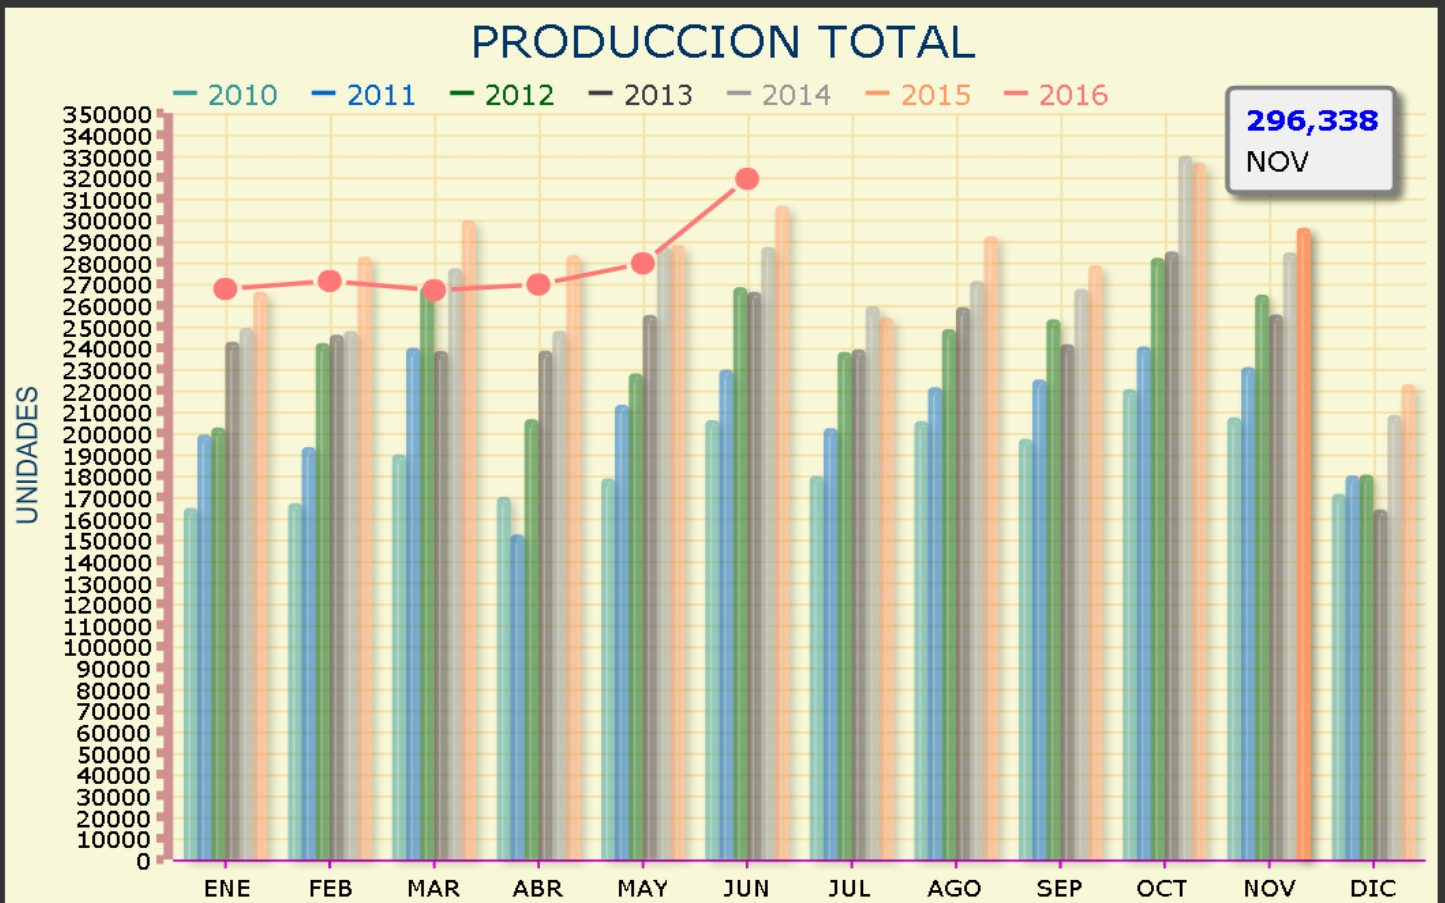
\includegraphics[width=0.7\textwidth]{introduccion/fig14.jpg}
\caption{Gráfica de producción total de vehículos en México \cite{UPS-16}. }
\label{Fcero1}
\end{figure}

En un artículo, la revisar Forbes (\cite{UPS-15}). Anuncio que un estudio de la Consultora IHS arrojó que se espera un crecimiento de 32 \% en la venta de vehículos para el 2021 a nivel mundial comparado con el periodo 2006-2013(557 millones de vehículos), esto hace que la innovación y la optimización de los mismos sea de gran importancia.\\

En la actualidad los automóviles cuentan con una serie de unidades de control que incluyen microprocesadores, tales como la unidad de control del motor, sistema de trasmisión, \textit{airbags}, sistemas de frenos, entre otros.\\


\subsection{DESCRIPCIÓN DEL PROBLEMA}

Actualmente en México se observan muchos vehículos de gama baja que se están deteriorando con el paso del tiempo sin que las personas tengan la intención de repararlos, debido a la gran posibilidad de financiar un carro de mejores características en cuestión de seguridad y confort, aunque implique un gran gasto mediante un plazo largo de cuotas.\\

Esta situación con lleva a una economía más ajustada debido al financiamiento de las agencias vehiculares y los intereses, además de que las personas que desean continuar con su vehículo actual no han encontrado un centro de servicio automotriz que trabaje bajo un método para aumentar las características del vehículo e incorporarle tecnología accesible en respecto a la seguridad y confort del usuario.\\

La compra de un modelo más reciente es la única forma de elevar la experiencia y seguridad del tripulante a la hora de viajar. En México el 46.2 \% de las personas según el Consejo Nacional de Evaluación de la Política de Desarrollo Social tiene pobreza (\cite{UPS-18}). A pesar de la situación económica del país, el registro de vehículos ha estado aumentando año tras año según las estadísticas de el Instituto Nacional de Estadística y Geografía (\cite{UPS-17}). Tal cual se muestra en la Figura \ref{Fcero2}. \\

\begin{figure}[H]
%\vspace{0.2cm}
\centering
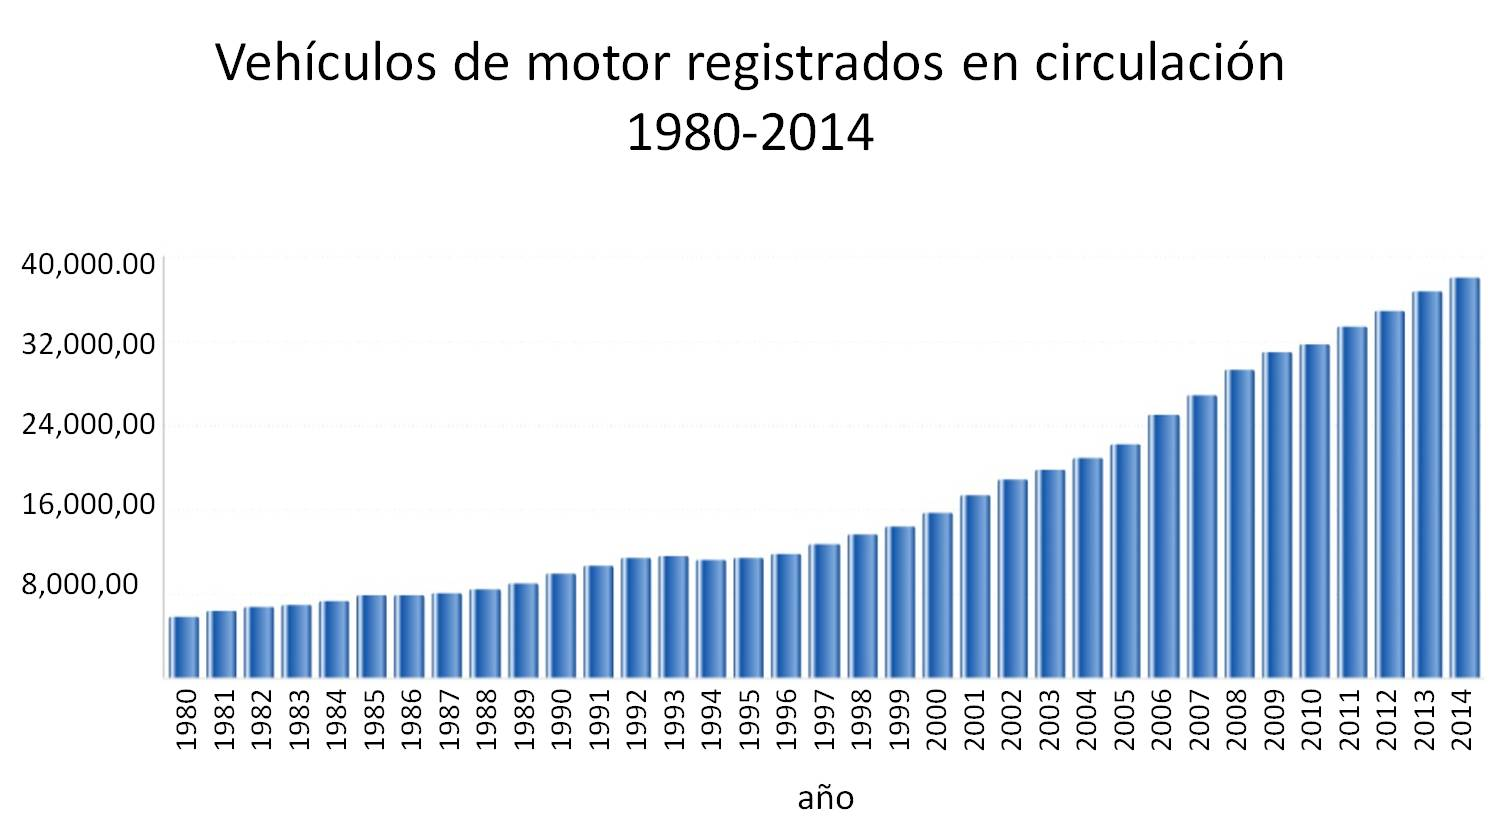
\includegraphics[width=1\textwidth]{introduccion/fig15.jpg}
\caption{Estadísticas de vehículos de motor registrados en circulación \cite{UPS-17}. }
\label{Fcero2}
\end{figure}



La compra de un vehículo modelo más reciente provoca una gran satisfacción durante su uso, sin embargo, el costo se eleva significativamente a su vez que la tecnología se va incluyendo, esto debido al encarecimiento en la compra de algunas piezas o sensores necesarios para el óptimo trabajo del vehículo. \\

También existe un factor muy importante para la economía de los mexicanos que es el alto índice de robos de los vehículos según la Asociación Mexicana de Instituciones de Seguros \cite{UPS-19} fueron 62 mil 533 unidades de autos asegurados robados en el 2015 y para la población es un descontrol económico el adquirir un vehículo sin una planificación de compra.\\



\subsection{JUSTIFICACIÓN}
Las agencias automotrices han procurado desarrollar vehículos con diferente cantidad de tecnología enfocada en el sistema de confort, a pesar de que no es mucha la diferencia de tecnología el precio que encarece el producto es notable.\\

El desarrollar una metodología que permita incluir tecnología actual a vehículos de gama baja y modelos anteriores es una gran oportunidad para que las personas puedan seguir usando su vehículo sin la necesidad de buscar otro por falta de tecnología, seguridad y comodidad.  \\

El restaurar un vehículo actualmente es costo y el valor en el mercado es muy bajo, en cambio si se le agrega tecnología puede llegar a cambiar el nivel de la gama e incluso aumentar el costo en el mercado, aprovechando que la industria automotriz es considerada uno de los pilares de la segunda más grande economía de América Latina y México es uno de los mayores exportadores de vehículos del mundo, según la revista Forbes (\cite{UPS-20}). Además, en otro artículo (\cite{UPS-21}), la revista Forbes menciona que mientras en América Latina las ventas automotrices reportan números rojos, en México crecen 17 \% en el 2015. \\

\subsection{ESTADO DEL ARTE}
Existen trabajos relacionados con incluir tecnología para optimizar, manipular y/o monitorear algún sensor o actuador del vehículo, se consultaron documentos científicos revisando las propuestas, resultados y limitaciones de algunas investigaciones con la finalidad de encontrar trabajos relacionados con los temas de seguridad, confort, monitoreo, automatización y comunicación.\\

Se ha encontrado una gran cantidad de proyectos vehiculares utilizando el sistema global para las comunicaciones móviles (GSM del inglés \textit{Global System for Mobile Communication}) (\cite{UPS-01,UPS-03,UPS-04,UPS-05,UPS-07}). La tecnología GSM permite la manipulación a distancia y es un reto que varios investigadores han aceptado en la actualidad.\\

Ángel Cornejo y Jorge Tintín en el 2010 (\cite{UPS-01}), desarrollaron e implementaron un sistema de telemetría a través de la tecnología GSM en un vehículo Chevrolet OPTRA 2008 monitoreando los parámetros de: i) temperatura, ii) presión de aceite, iii) velocidad de giro del motor y iv) velocidad de desplazamiento. El sistema se construyó mediante tecnología GSM, utilizaron un dispositivo móvil para conectar a la tarjeta electrónica, como medio de comunicación debido al alcance de cobertura de la red móvil. Sin embargo, se tiene un costo por cada acción, para tener en perfecto estado la comunicación Ángel recomienda tener activo un paquete ilimitado de mensajes de texto ya que el agotamiento del servicio de mensajería simple (SMS del inglés \textit{Short Message Service}) provocaría errores en la recepción y envío de datos.\\

En el 2012 Fabián Arancibia y Claudio Urrea (\cite{UPS-02}), implementaron un sistema de teleoperación en un carro de golf eléctrico con la finalidad de sentar las bases para la experimentación e implementación de sistemas de teleoperación. Se realizó un proyecto el cual está constituido por tres bloques básicos los cuales se muestran en la Figura \ref{Funo}. Una combinación un \textit{joystick}, enrutador Wifi, la placa de Arduino Mega y una interfaz electrónica que en conjunto sirve para manejar los actuadores del volante, los pedales, las luces y la bocina.  Utilizando cámaras de red para obtener retroalimentación y visualizar con un margen de retardo de un segundo. Sin embargo, es necesario estar cerca de una red Wifi para poder acceder al sistema de control remoto.\\

%
\begin{figure}[H]
%\vspace{0.2cm}
\centering
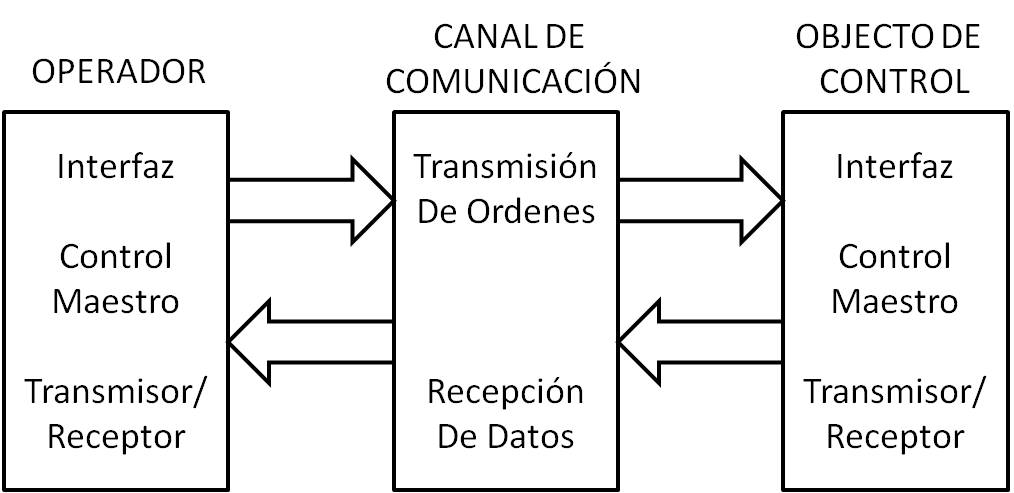
\includegraphics[width=0.6\textwidth]{introduccion/fig1.jpg}
\caption{Diagrama de bloques del sistema. }
\label{Funo}
\end{figure}
%

El tema de seguridad vehicular se ha trabajado sobre la cuestión para bloquear y desbloquear de manera física o mediante un SMS el sistema de encendido del vehículo (\cite{UPS-03,UPS-04,UPS-09}). Utilizando un dispositivo móvil que se encarge de enviar una señal para activar o desactivar un relevador automotriz es un caso específico. Este desarrollo se realizó en el 2010 por el Juan Cujano en (\cite{UPS-03}), y menciona la necesidad de contar con un celular conectado al vehículo el cual reciba los mensajes enviados por el usuario y mediante un micro controlador programado junto con relevadores, capacitores y resistencias formando una placa electrónica con diseño propio, esta sirve para controlar la acción hacia el automóvil, por tal motivo tiende a tener la misma limitación que el proyecto de Ángel Cornejo y Jorge Tintín, respecto a la limitacion  se recomienda tener SMS ilimitados.\\

Geovanny Chuqui dice en el 2011 (\cite{UPS-04}), que aparte del bloqueo o desbloqueo del encendido propone agregar características relacionadas para evitar el robo del vehículo mediante la manipulación de los actuadores de los seguros de las puertas, además de que en caso de no ser el propietario quien habrá el vehículo se envié una notificación. También menciona que utiliza el sensor del velocímetro para después de 30 metros recorridos de manera automática los seguros se activen. Geovanny está muy enfocado sobre el tema de seguridad, la propuesta es buena y es una gran base para realizar proyectos afines a mejorar las características del vehículo.\\

En mayo del 2016 (\cite{UPS-05}), Carlos Cuadrado y Gerardo Aranguren han estado trabajando en la Universidad de País Vasco/Euskal Herriko Unibertsitatea con un sistema de telecontrol, este consta de un módulo GSM para el enlace a la red telefónica digital y por una tarjeta de conexión al equipo controlado. En el procesador de la tarjeta se encuentran programadas las funciones de control. Y mediante mensajes SMS se envían órdenes de control y se recibe información de monitoreo sobre el estado del equipo. Este sistema propone soluciones domóticas mediante el funcionamiento que se muestra en la Figura \ref{Ftres}, enfocado a máquinas industriales alejadas del puesto de mando, expendedoras, automóviles, soluciones domóticas entre otras. Aunque se puede comentar que la necesidad de manipular este tipo de maquinaria es real, también puede ser requerido estar a cierta distancia, el analiza la posibilidad de utilizar tecnología Wifi o Bluetooth, perimiendo así el reducir el gasto económico por cada instrucción enviada y recibida.\\

%
\begin{figure}[H]
%\vspace{0.2cm}
\centering
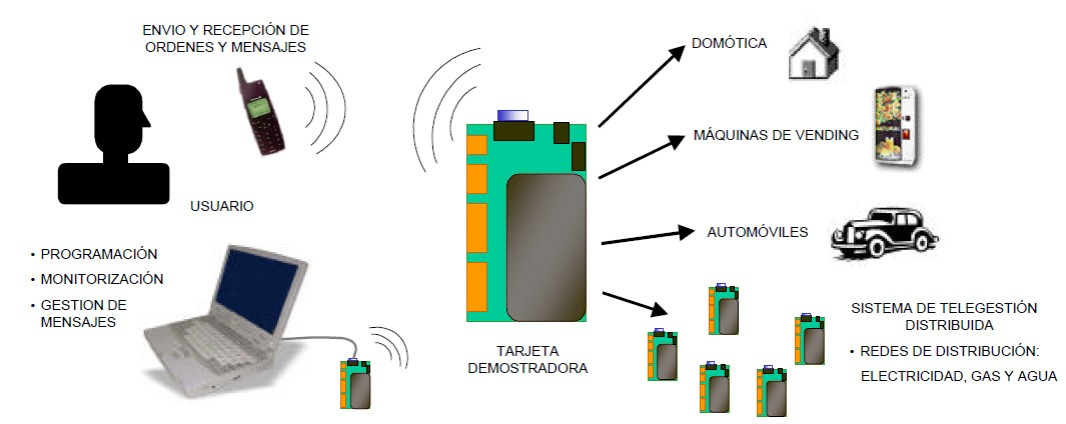
\includegraphics[width=1\textwidth]{introduccion/fig3.jpg}
\caption{Esquema del funcionamiento del sistema de telecontrol \cite{UPS-05}. }
\label{Ftres}
\end{figure}
%

Existe una gran cantidad de proyectos que se pueden implementar en diferentes equipos (\cite{UPS-05,UPS-06}). En el caso de los vehículos, Luis Miguel Ruiz (\cite{UPS-06}) en septiembre del 2015 presentó su tema de fin de grado el cual describe la instalación de sistemas de seguridad pasiva en un vehículo clásico perteneciente a la gama baja. Él explica que estos sistemas están conformados de tecnología accesible en estos tiempos, Luis la implementa en un vehículo MINI MORRIS 850 de 1972. Dichos sistemas son: i) alarma antirrobo, ii) ayuda al estacionarse, iii) monitorización de las revoluciones del motor y iv) encendido automático de luces. Este tema se ha llevado acabo principalmente con relevadores, sensores de distancia y la tarjeta programable Arduino, desarrollando un diagrama de flujo para plasmar las actividades generales como se muestra en la Figura \ref{Ftresdos}, sin embargo, a pesar de que es una idea muy interesante puede carecer de detalles de análisis para controlar los sistemas de una manera más eficiente, sin mencionar la cantidad de proyectos realizados similares con la tarjeta Arduino.\\

%
\begin{figure}[H]
%\vspace{0.2cm}
\centering
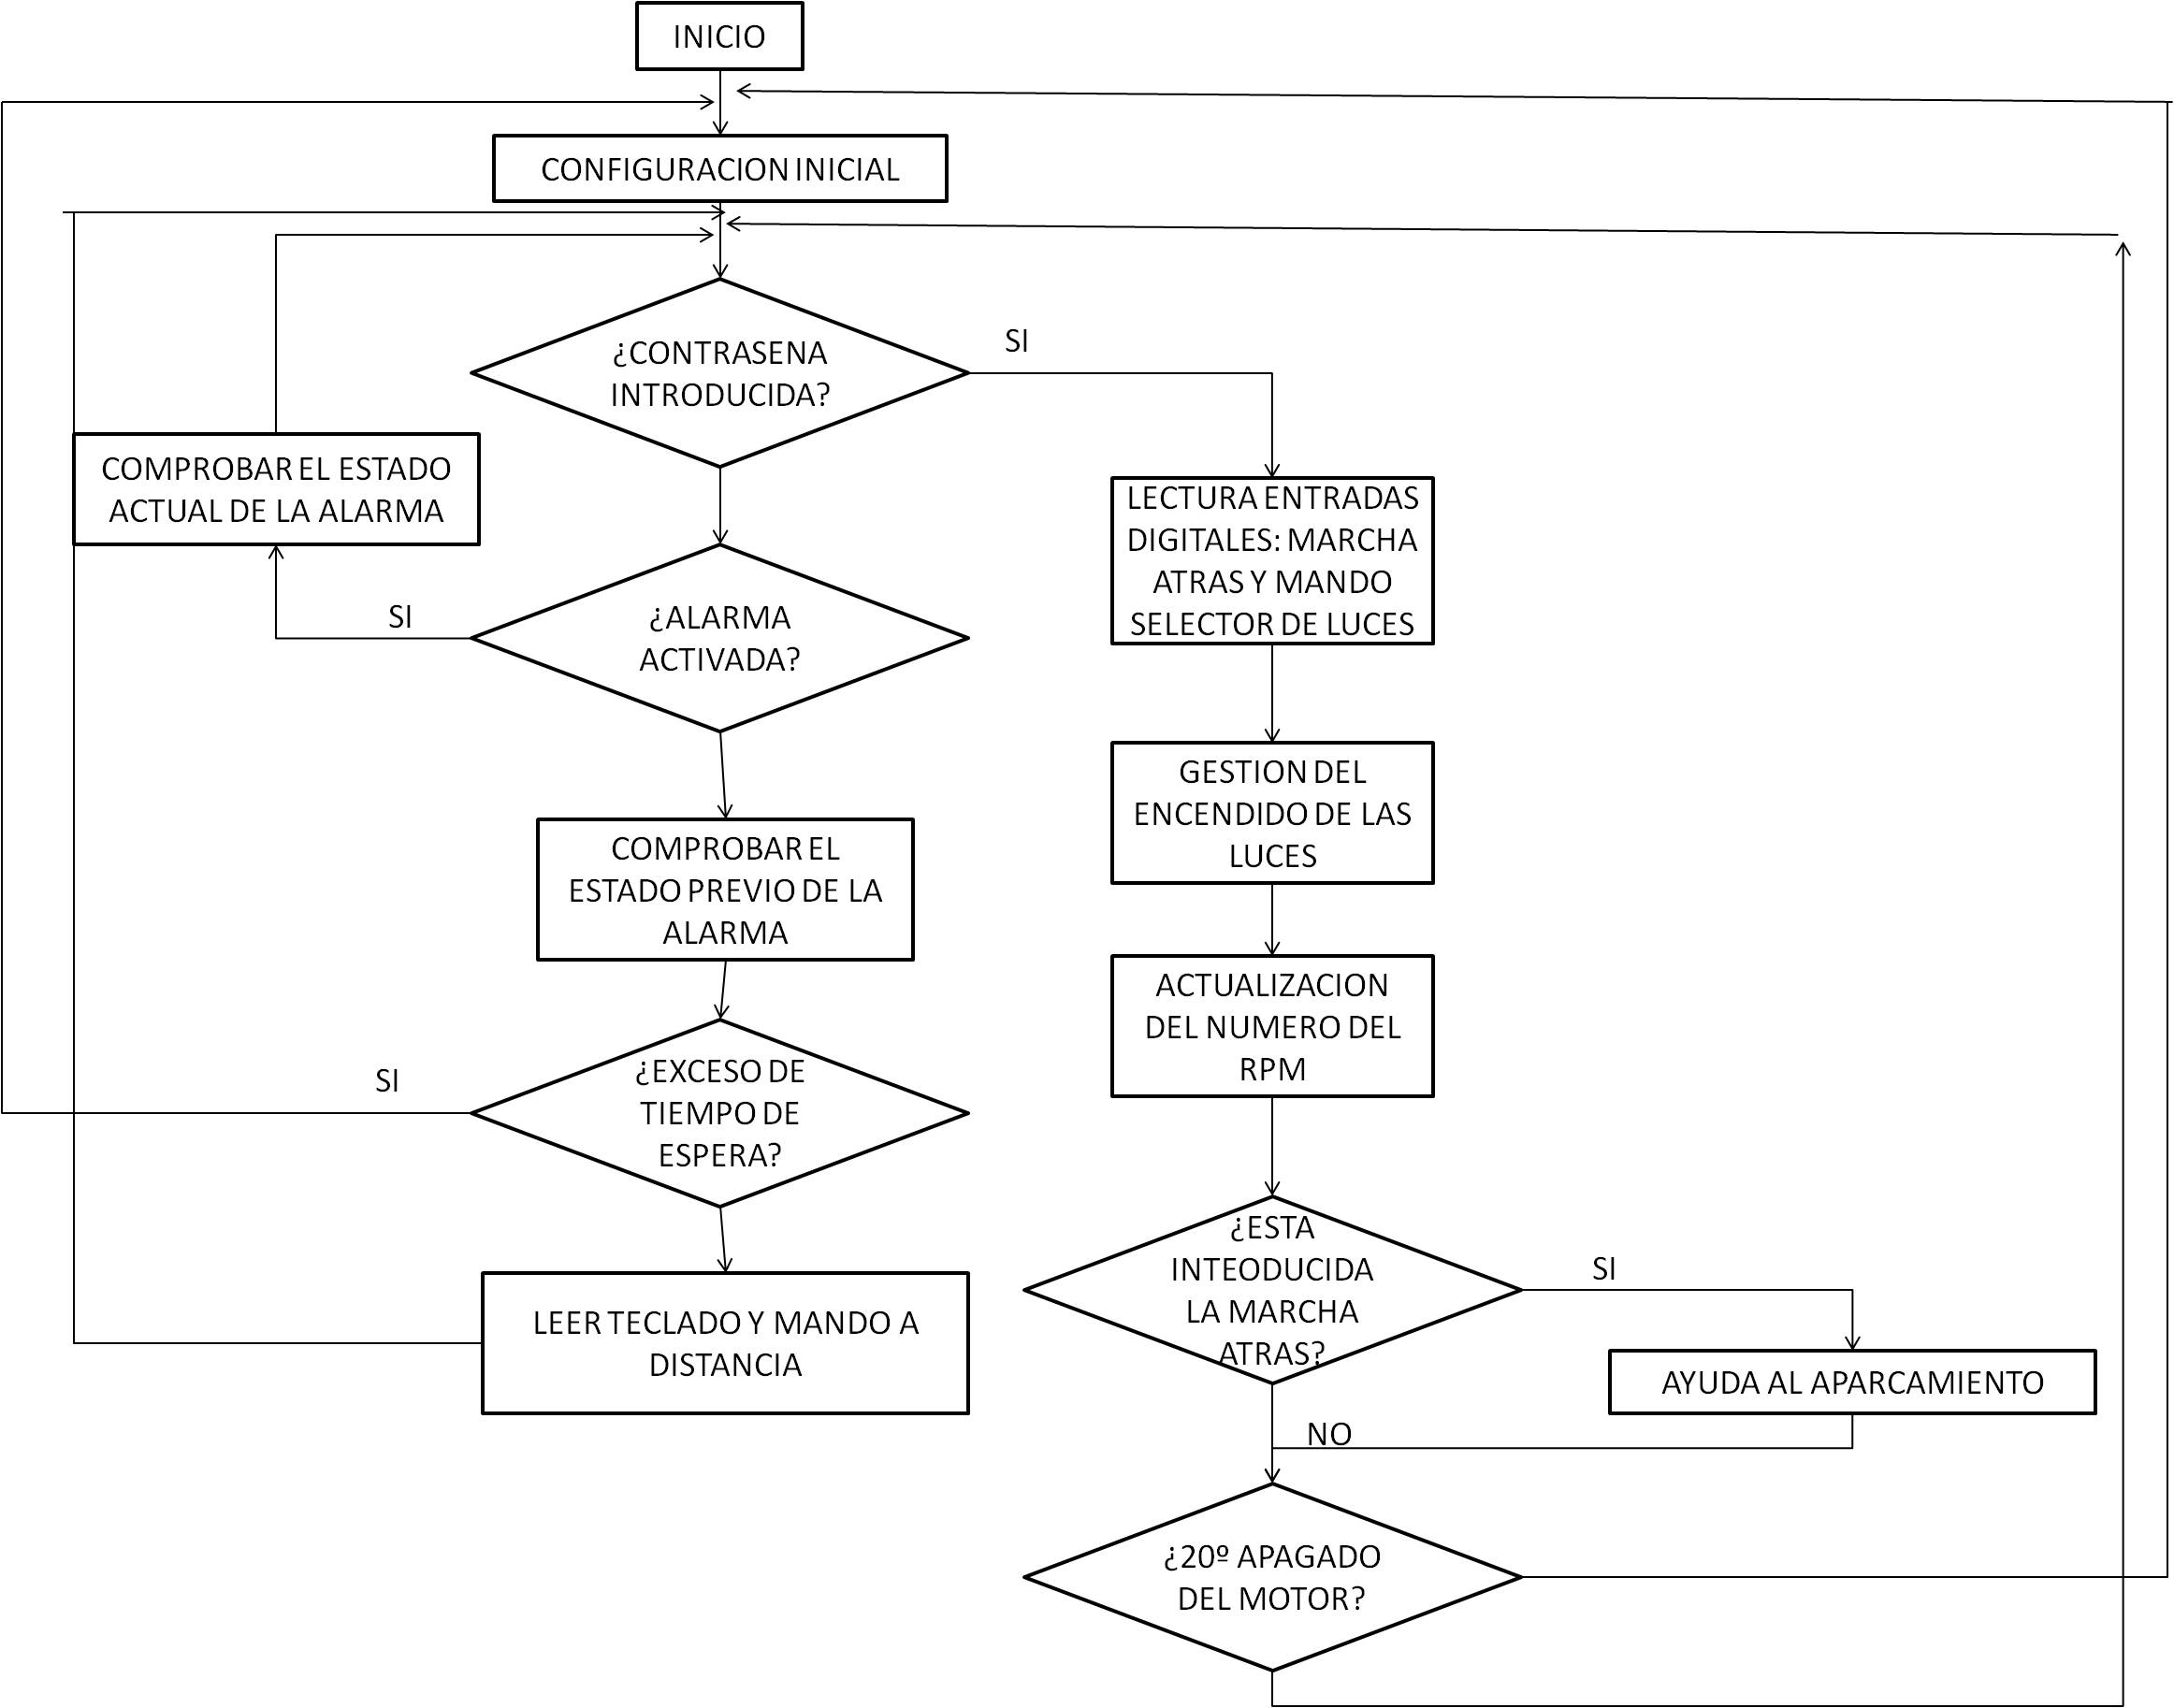
\includegraphics[width=0.8\textwidth]{introduccion/fig5.jpg}
\caption{Vista general del diagrama de flujo del programa. }
\label{Ftresdos}
\end{figure}
%

Por otra parte, existen aplicaciones móviles enfocadas en vehículos de gama media y alta (\cite{UPS-07,UPS-08}), los vehículos definidos en estas gamas contienen el sistema diagnóstico a bordo II (OBD del inglés \textit{On Board Diagnostic}). El sistema \textit{OBD} permite la comunicación entre los sensores del sistema de tracción. Miriam Loachamín en octubre del 2015 (\cite{UPS-07}) desarrollo su trabajo enfocado al monitoreo de parámetros mediante el dispositivo Arduino y la librería OBD.h, donde esta permite la lectura de códigos del sistema \textit{OBD II}. El dispositivo Arduino envía y recibe la señal con la tecnología de comunicación de los celulares GSM y lo representa por medio de un diagrama de bloques del sistema, el cual se muestra en la Figura \ref{Fcuatro}. Por otro lado, el dispositivo ELM 327 se inserta en el conector de enlace de datos para enviar las señales que obtiene de los sensores del vehículo. El ELM 327 únicamente permite únicamente el monitoreo de ciertos sensores del sistema de tracción del vehículo, no permite la comunicación con actuadores para su manipulación.\\

%
\begin{figure}[H]
%\vspace{0.2cm}
\centering
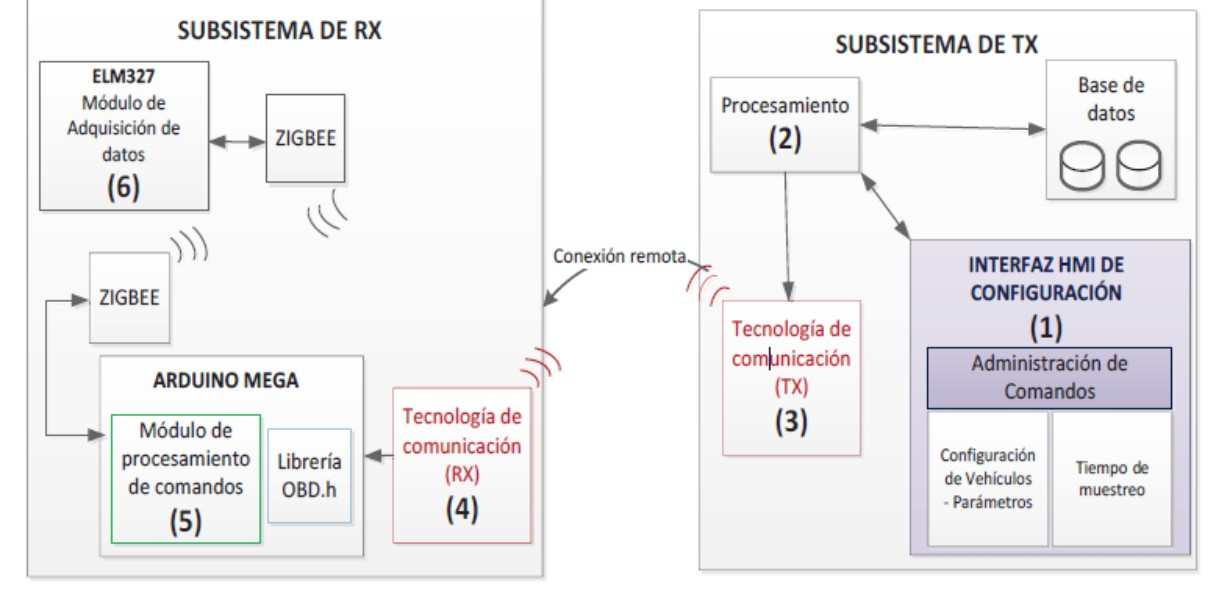
\includegraphics[width=0.8\textwidth]{introduccion/fig6.jpg}
\caption{Diagrama de bloques del sistema de administración remota propuesto \cite{UPS-07}. }
\label{Fcuatro}
\end{figure}
%


En septiembre del 2015 Virgilio García trabajó con un vehículo (\cite{UPS-08}), utilizó la tarjeta electrónica ELM 327 junto con una tarjeta Raspberry Pi que implemento al vehículo. Esta adaptación permitió incorporar de manera independiente al vehículo, los sensores de temperatura y monóxido de carbono, con un sistema de notificación en caso de información inusual. Virgilio se basa principalmente en el desarrollo de una aplicación móvil para sistema operativo Android en donde puede medir la temperatura interior con un historial de la temperatura por fecha, tal como se muestra en la Figura \ref{Fcinco}, donde utiliza la tecnología Bluetooth como medio de comunicación. Este trabajo al igual que el tema de Miriam Loachamín utilizan la librería OBD.h que contiene la información de los códigos del sistema de tracción, aunque no permite la modificación de ningún parámetro del sensor o actuador, simplemente es el monitoreo de ciertos sensores dependiendo el vehículo.\\

%
\begin{figure}[H]
%\vspace{0.2cm}
\centering
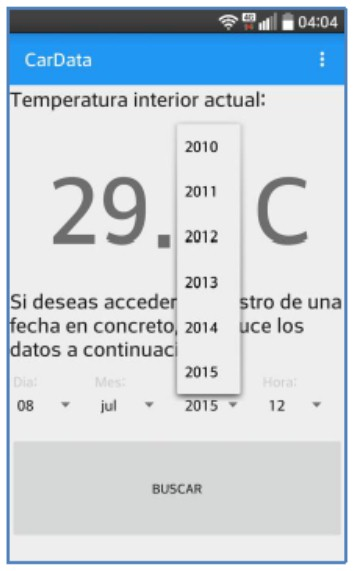
\includegraphics[width=0.3\textwidth]{introduccion/fig7.jpg}
\caption{Interaz que muestra el historial de la temperatura del vehículo \cite{UPS-08}. }
\label{Fcinco}
\end{figure}
%

Jesús Castillo y colaboradores trabajaron en el 2015 (\cite{UPS-10}), con el tema relacionado al sistema de seguridad activa que comprende de los sistemas antibloqueo de frenos, control de tracción y de control de estabilidad. Proponen detectar las condiciones de la carretera por donde pasa el vehículo utilizando sensores estándar como los vehículos, buscando estimaciones en tiempo real sobre la fuerza de contacto entre la rueda, la carretera y la velocidad. Obtuvieron un algoritmo de estimación de parámetros y mediante leyes físicas y cálculos matemáticos realizaron un esquema de cálculo, tal cual se muestra en la Figura \ref{Fcincodos} para obtener el deslizamiento y el coeficiente de fricción y a partir de esos datos el estado de la carretera y el deslizamiento óptimo de la superficie en la que el vehículo está circulando. Además, estos parámetros son fundamentales para los sistemas de seguridad activa o de la conducción automática del controlador para una reacción más rápida y con más facilidad a situaciones inesperadas y peligrosas.\\

%
\begin{figure}[H]
%\vspace{0.2cm}
\centering
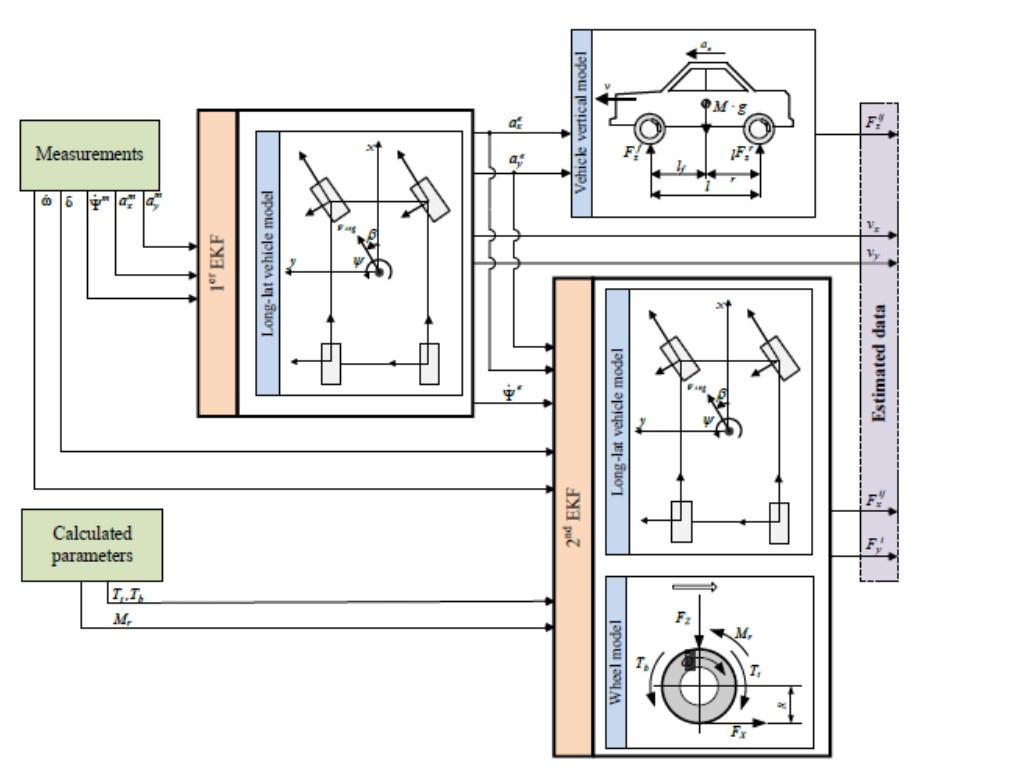
\includegraphics[width=0.7\textwidth]{introduccion/fig8.jpg}
\caption{Esquema del algoritmo estimado \cite{UPS-10}. }
\label{Fcincodos}
\end{figure}
%


En el 2012 se presentó un artículo a cargo de Jorge Capra y colaboradores (\cite{UPS-13}), sobre la detección de vehículos robados en Argentina, por medio del reconocimiento automático de las placas usando un reconocedor óptico tal cual se muestra en la Figura \ref{Fseis}. Sin embargo, gran parte del trabajo se realizó en un ambiente controlado y existen dificultades para detectar caracteres cuando hay poco contraste o la iluminación no es homogénea o con demasiada perspectiva. Este trabajo puede tener varias funcionalidades además del control vehicular como por ejemplo, en operativos de inspección policial, identificación en puestos de peajes y control de estacionamiento, entre otros.\\

%
\begin{figure}[H]
%\vspace{0.2cm}
\centering
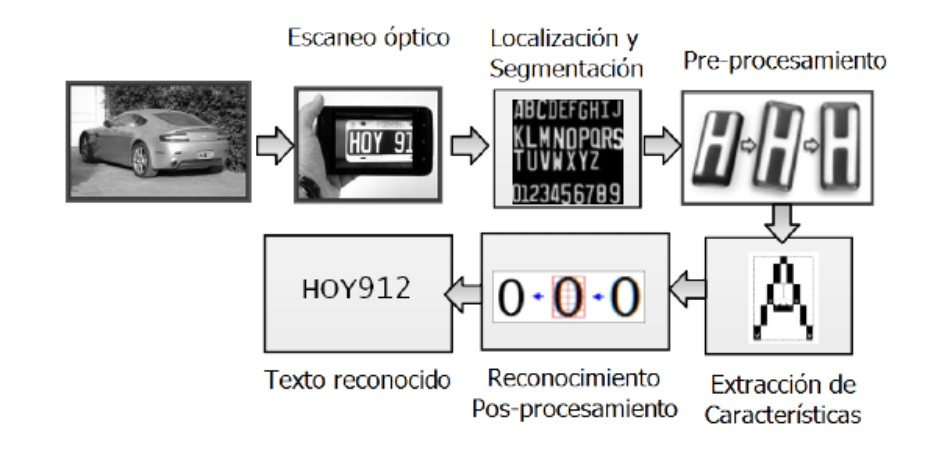
\includegraphics[width=0.7\textwidth]{introduccion/fig9.jpg}
\caption{Esquema del algoritmo estimado \cite{UPS-13}. }
\label{Fseis}
\end{figure}
%

El bloqueo y desbloqueo electrónico por huella dactilar es un proyecto de Luis Eduardo Cando (\cite{UPS-09} ), en donde se pretende tener un mayor nivel de seguridad al instante de encender el automóvil, mediante un módulo biométrico y una pantalla para visualizar la interfaz entre el vehículo y el módulo, buscando el encendido del vehículo soló por personas dadas de alta en el sistema de control. Las pruebas que se realizaron en este trabajo describen el buen funcionamiento de la huella o conocer el código pin del módulo biométrico, mostrando el diagrama general, además del costo equivalente a  837.70 USD para la implementación del proyecto. Sin embargo, para este proyecto es indispensable los relevadores automotrices, dejando la oportunidad a un experto en mecánica o electrónica poder desconectar con facilidad la seguridad.\\


Edwin Ismael en diciembre del 2015 (\cite{UPS-11}), trabajó en un proyecto para el control del sistema de iluminación, accionamiento de ventanillas, limpiaparabrisas, calefacción por medio de comandos de voz y una tarjeta electrónica con base en Arduino. En las conclusiones muestran la necesidad de un acumulador en buen estado y habla sobre las limitaciones actuales del comando por voz, debido a que existen muchos factores que alteran la tonalidad de la voz provocando dificultades para ejecutar los comandos. \\


En el 2013 Oswaldo Quito y Benito Sarmiento (\cite{UPS-12}), desarrollaron un sistema para obtener su grado de ingeniería donde controlan algunas actividades del vehículo Luv Clásica de la marca Chevrolet mediante SMS, utiliza la tecnología GPS para localizar la camioneta cuando se requiera. De igual forma se puede bloquear por medio del GPS en cualquier lugar donde se encuentre. Oswaldo y Benito nos muestran su esquema general en la Figura \ref{Fnueve}, también corta el combustible directamente de la camioneta, además de un panel para configurar el sistema y por medio de un relevador se puede bloquear el encendido electrónico.\\

%
\begin{figure}[H]
%\vspace{0.2cm}
\centering
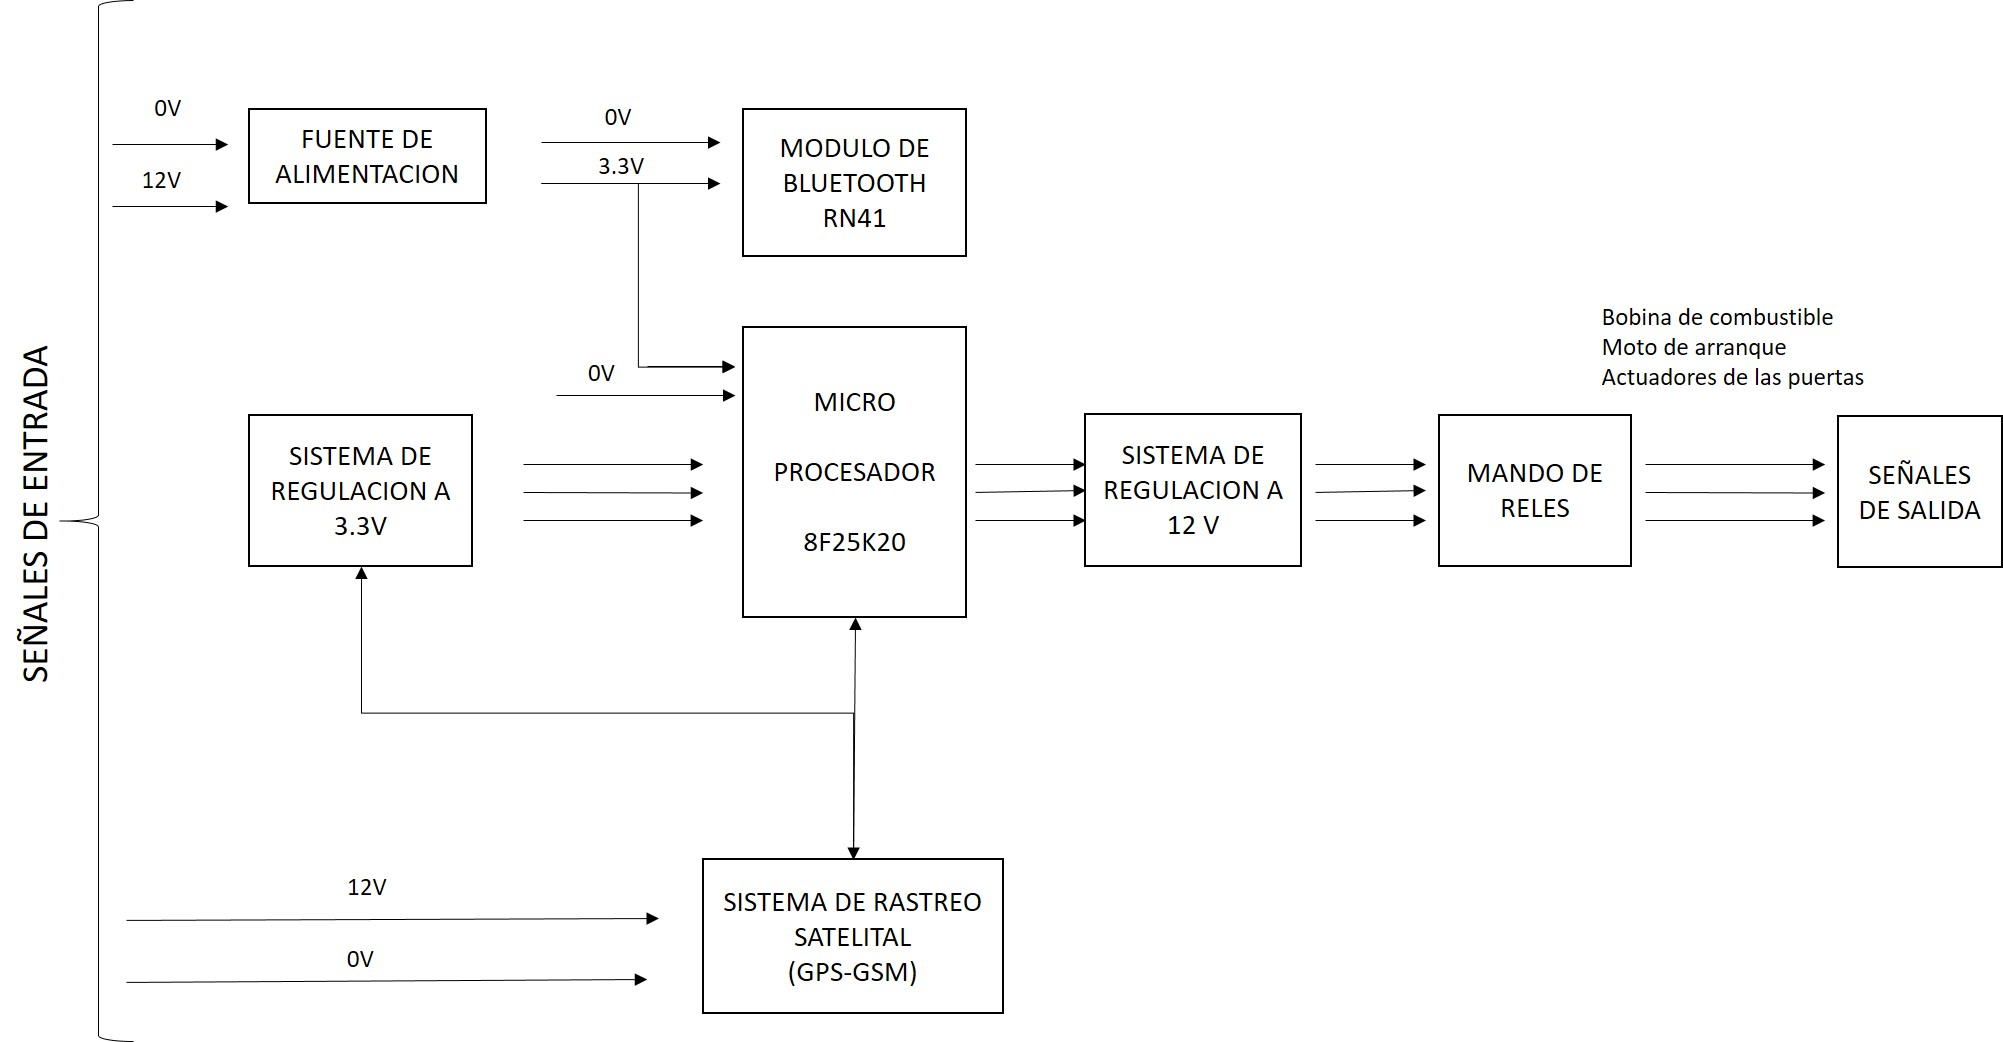
\includegraphics[width=0.6\textwidth]{introduccion/fig12.jpg}
\caption{Esquema del circuito electrónico \cite{UPS-12}. }
\label{Fnueve}
\end{figure}
%

Roberto Carlos Paredes (\cite{UPS-14}), trabajo en el 2014 con un proyecto de seguridad, que permite detectar mediante sensores de presión cuando una persona está ocupando el asiento del piloto o copiloto y con un sensor de proximidad magnético se puede identificar si la persona tiene puesto el cinturón de seguridad cuando el vehículo ya este encendido, utilizando un sistema de reproducción MP3 para emitir un aviso. Roberto nos muestra una imagen de la implementación en la Figura \ref{Fdiez}\\

%
\begin{figure}[H]
%\vspace{0.2cm}
\centering
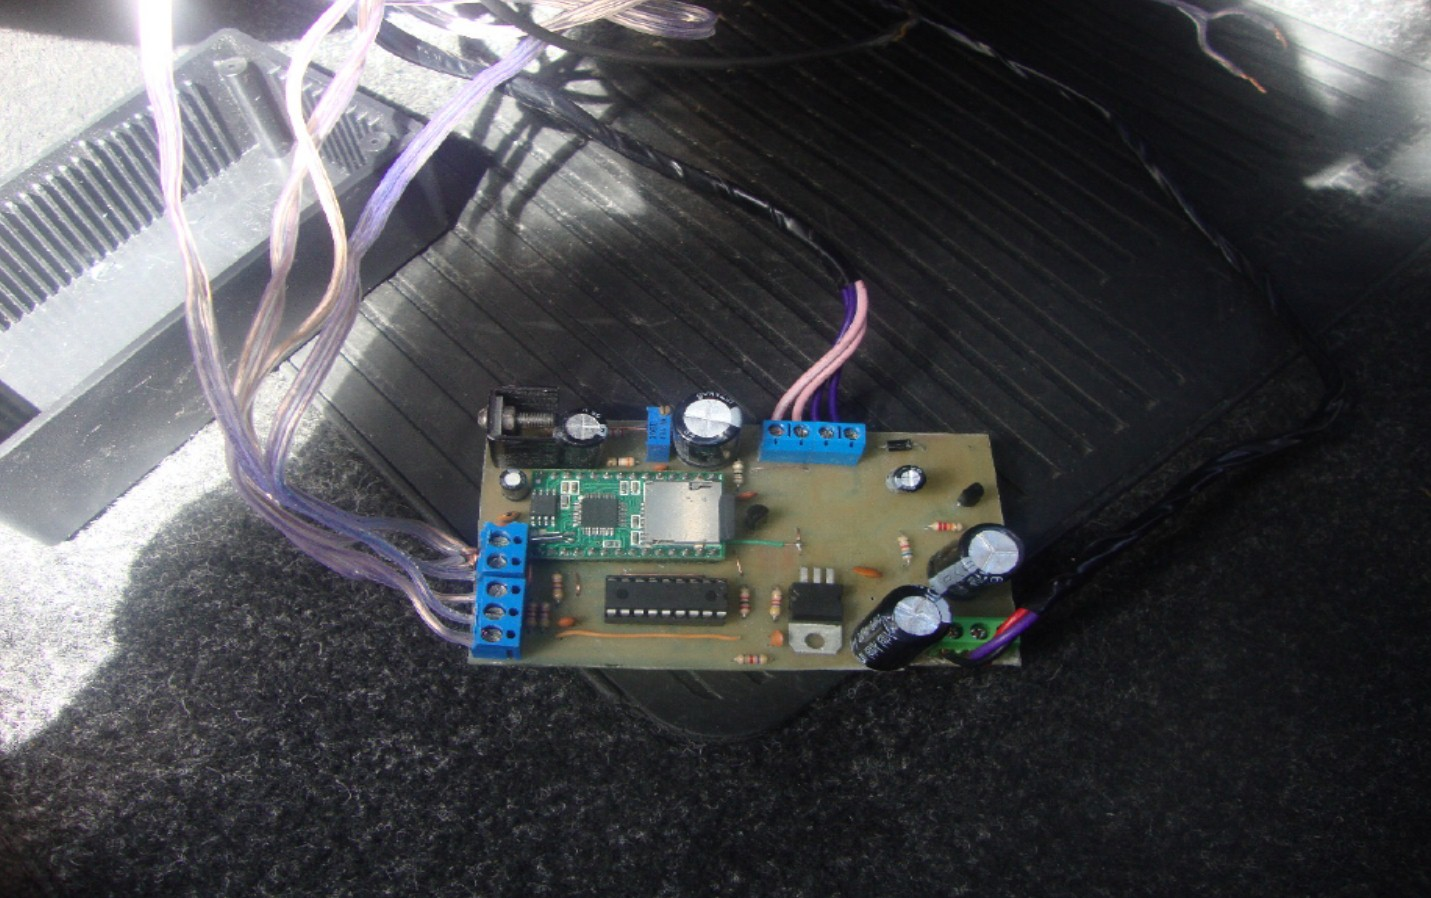
\includegraphics[width=0.6\textwidth]{introduccion/fig13.jpg}
\caption{Placa electrónica Conectada al vehículo \cite{UPS-14}. }
\label{Fdiez}
\end{figure}
%

Otro de los trabajos que se realizó fueron algunas actividades con el sistema \textit{OBD} II y el \textit{CAN-BUS} de datos (\cite{GB1}), desarrollando la siguiente hipotesis. La solución que se propone es el desarrollo de una aplicación móvil mediante plataforma Android para poder modificar algunos parámetros y sensores del Sistema de Confort de un Vehículo de Gama media, utilizando de vehículo de pruebas un Stratus XLS 2006. \\

Las actividades que se desarrollaron fueron enfocadas a realizar pruebas en sistemas existentes en el mercado, estas se enlistan acotinuación:

\begin{itemize}
\item Funcionamiento del Can Bus y el conector DCL,
\item Funcionamiento del dispositivo EML327,
\item Funcionamiento de aplicaciones móviles,
\item Codificación y descodificación de la señal,
\item Pruebas y Resultados.
\end{itemize}

\paragraph{Funcionamiento del Can Bus y el conector DCL}
El desarrollo de esta actividad se llevó a cabo mediante la investigación de la metodología sobre el Sistema eléctrico del vehículo (\cite{GB1}), el can bus es el encargado de transmitir los códigos de falla del vehículo y el conector OBD, también conocido como conector de enlace de datos es el encargado pasar por medio de algún escáner los códigos al usuario, está ubicado normalmente en la parte inferior del volante.\\

Durante esta actividad también se realizaron pruebas con el osciloscopio, detectando los pines encargados de transmitir las señales por medio del CAN Bus, también denominados CAN \textit{High} y CAN \textit{Low}, los pines correspondientes son el número 2 y el 10, tal y como se muestra en la Figura \ref{Medos} debido a que cada marca maneja un protocolo ya establecido.

%
\begin{figure}[H]
%\vspace{0.2cm}
\centering
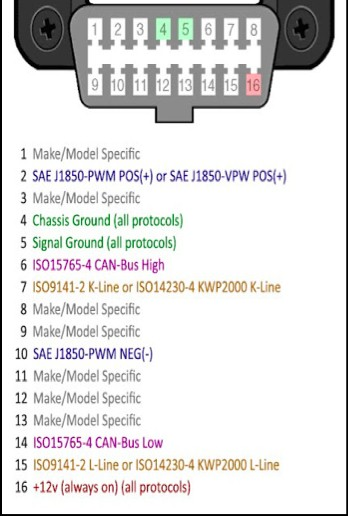
\includegraphics[width=0.3\textwidth]{metodologia/protocolos_obd.jpg}
\caption{Protocolos de comunicación con la configuración de los pines del conector DCL.}
\label{Medos}
\end{figure}
%

\paragraph{Funcionamiento del dispositivo EML327}

En la siguiente actividad se probaron algunas aplicaciones móviles existentes en el mercado para poder verificar por cuenta propia que el sistema Can Bus es capaz de enviar información relevante para el usuario a la hora de viajar en el vehículo (\cite{GB2}).\\

Por lo cual se realizaron pruebas con el escáner EML327, sin embargo este escáner funciona únicamente  para el sistema de tracción, esto permitió realizar las primeras pruebas en el vehículo sobre el escaneo de información a una aplicación móvil mediante tecnología Bluetooth. \\

Primeramente se conectó el EML327 al conector de enlace de datos tal cual se muestra en la Figura \ref{Metres}\\

%
\begin{figure}[H]
%\vspace{0.2cm}
\centering
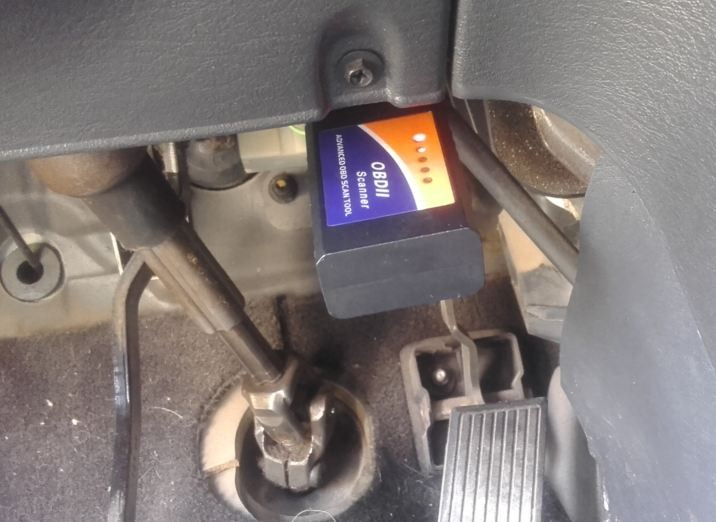
\includegraphics[width=0.5\textwidth]{metodologia/elm327.jpg}
\caption{dispositivo EML 327 conectado al vehículo.}
\label{Metres}
\end{figure}


\paragraph{Funcionamiento de aplicaciones móviles}

Después se buscó en la tienda de Google Play aplicaciones compatibles con el escáner EML327, se obtuvieron dos aplicaciones``Scanner OBD" y ``Piston”, se descargaron y se procedió a visualizar el funcionamiento de ambas. La aplicación Escáner OBD muestra información sobre el protocolo de comunicación la cual se muestran en las Figuras \ref{Mecuatro}. 

\begin{figure}[H]
\centering
\subfigure[]{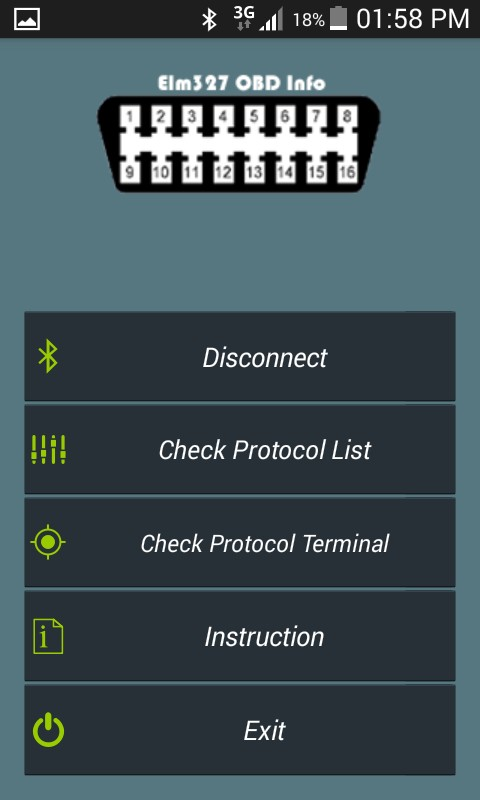
\includegraphics[width=60mm]{metodologia/eml327.jpg}}\hspace{10mm}
\subfigure[]{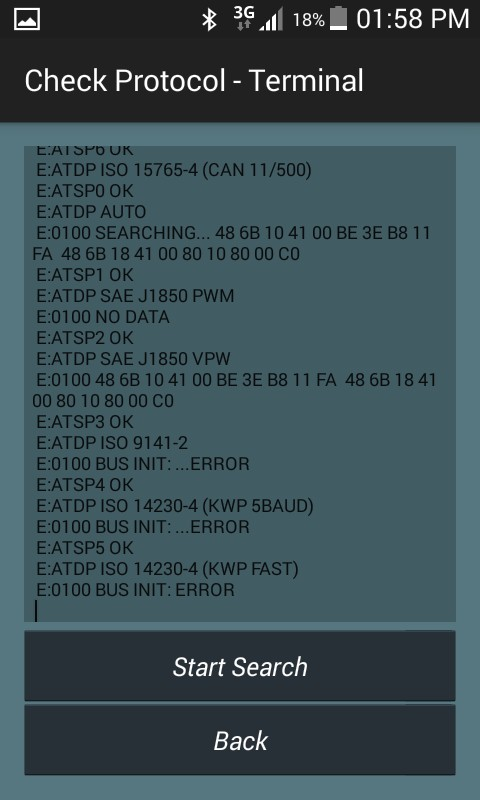
\includegraphics[width=60mm]{metodologia/eml327_.jpg}}
\caption{Pantallazos de la aplicación Scanner OBD.} \label{Mecuatro}
\end{figure}


La aplicación “Piston” muestra información sobre el sistema de tracción como el voltaje de la batería, la temperatura del agua, las revoluciones por minuto y la velocidad, tal cual se muestra en la Figura \ref{Mecinco}.

\begin{figure}[H]
\centering
{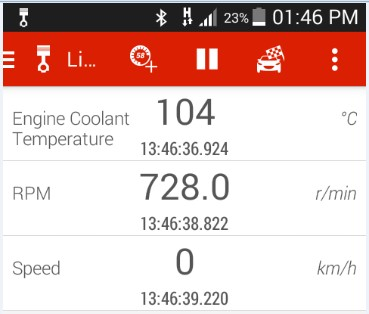
\includegraphics[width=0.6\textwidth]{metodologia/piston.jpg}}
\caption{Pantallazo de la aplicación Piston.} \label{Mecinco}
\end{figure}



\paragraph{Codificación y descodificación de la señal}

Para esta actividad, se vio en la necesidad de conocer completamente el sistema de confort, principalmente en la parte del sistema eléctrico. \\

Por protocolos de seguridad las armadoras no permiten el acceso al mismo, sin embargo algunas asociaciones de mecánicos en el país tienen acceso a ellos mediante software que los auxilia a reparar los vehículo, como es el caso del software OnDemand5 (\cite{GB3}).\\


\subsection{OBJETIVOS}
\subsubsection{Objetivo General}
Incrementar la comodidad y la seguridad de vehículos de gama baja mediante la implementación de actuadores manipulados por una aplicación móvil para el monitoreo de la emisión de algunos gases y aumentar la comodidad y seguridad del tripulante.


\subsubsection{Metas específicas}
  \begin{itemize}
           \item Diseñar una estructura de comunicación entre los actuadores y la aplicación móvil
\item Instrumentar los actuadores seleccionados
\item Diseñar el circuito electrónico
\item Desarrollar la aplicación móvil
  \end{itemize}



\subsection{SOLUCIÓN PROPUESTA}
Desarrollar una metodología que permita aumentar la comodidad y seguridad para el tripulante por medio de la incorporación de tecnología en vehículos de gama baja y modelos anteriores.\\

Mediante la tecnología de bluetooth se comunica una aplicación móvil a una tarjeta electrónica dentro del vehículo que permita manipular los actuadores del vehículo pertenecientes al sistema de confort y tracción del vehículo.\\

\subsection{DESCRIPCIÓN DEL DOCUMENTO}

Capítulo 2 muestra el marco teórico referente a comprender mejor el proyecto con temas involucrados como es el caso de los tipos de aplicación, los medios de comunicación, las tarjetas electrónicas que existen en el mercado para desarrollar proyectos las áreas de mejora continua del vehículo, entre otros. En el capítulo 3 denominado metodología se muestra el proceso que se realizó para llevar de una manera efectiva y replicable el proyecto incluyendo la implementación de los actuadores y la instalación de la aplicación móvil. En el capítulo 4 nombrado análisis de resultados se muestran los resultados que se obtuvieron y las evidencias relacionadas con la implementación y pruebas realizadas. Y en el capítulo 5 que es el de conclusiones y trabajo a futuro se muestran la opinión personal del proyecto analizando los resultados obtenido, su relevancia y aprendizaje durante el desarrollo del proyecto y algunos aspectos relacionados a las limitaciones, además de proponer líneas de investigación y propuestas para mejorar el proceso de instrumentación.


\clearpage
\section{MARCO TEÓRICO}

En este capítulo se describen los principales temas de interés para comprender de mejor manera el proyecto mediante fundamentos teóricos. Realizando una descripción de las tecnologías utilizadas para el desarrollo de la investigación. Es necesario comprender temas relacionados con los tipos de aplicaciones, dispositivos móviles, tecnologías de comunicación, tarjetas y componentes electrónicos, actuadores y sensores del vehículo, además de los diferentes aportes tecnológicos de la actualidad relacionados con la mejora continua del vehículo.


\subsection{TIPOS DE APLICACIONES}



\paragraph{Aplicaciones Web:}

(\cite{MT-11}) Son aquellas desarrolladas bajo lenguajes de desarrollo principalmente con tecnología Web entre los que destacan HTML, CSS y JavaScript. Hoy en día el trabajar con un \textit{framework} para el desarrollo eficientiza los procesos y permite la escalabilidad de la aplicación. Se podría decir que este tipo de aplicaciones son muy usadas para brindar accesibilidad a la información desde cualquier dispositivo móvil sin importar el sistema operativo, ya que solamente se necesita contar con un navegador para acceder a esta debido a que se encuentran alojadas en un servidor que mediante un nombre de dominio asociado o la dirección pública se pueden acceder. Algunas de las ventajas y desventajas de estas son: \\



Ventajas
\begin{itemize}
\item  Pueden ser utilizadas desde cualquier dispositivo móvil sin importar el sistema operativo.
\item  Puede que requiera un coste para su desarrollo, peor este puede ser mínimo en comparación con las nativas.
\item  No requieren de ninguna aprobación para su publicación.
\end{itemize}
Desventajas
\begin{itemize}
\item  No pueden ser publicadas en plataformas para su distribución.
\item  No utilizan los recursos del sistema ni del dispositivo de manera óptima.
\end{itemize}


\paragraph{Aplicaciones Móviles:}

una aplicación móvil (\cite{MT-11}), es una aplicación informática desarrollada para ser ejecutada a través de un dispositivo móvil inteligente, tablet o cualquier otro dispositivo que cuente con un sistema operativo. Estas se encuentran en tiendas en línea, por medio de las cuales son accedidas por el público que desee usarlas.\\

Dentro de estas plataformas de distribución de las aplicaciones móviles, se podrá encontrar de dos tipos, gratis y de paga. Las aplicaciones móviles pueden ser nativas que son aquellas desarrolladas bajo un lenguaje y entorno de desarrollo específico, lo cual permite, que su funcionamiento sea muy fluido y estable para el sistema operativo que fue creada. Pero también es importante recordar, que todo en esta vida tiene su ventajas y desventajas, y que las aplicaciones nativas no son la excepciona. Las ventajas y desventajas de estas son:\\

Ventajas
\begin{itemize}
\item  Utilización de los recursos tantos del sistema como del hardware.
\item  Permite ser publicada en tiendas para su distribución.
\item  En su mayoría, no necesitan estar conectadas a Internet para su funcionamiento.
\end{itemize}

Desventajas
\begin{itemize}
\item  Solo pueden ser utilizadas por un dispositivo que cuente con el sistema para el cual fue desarrollada.
\item  Requiere de un costo para distribuirla en una tienda, y dependiendo el sistema, para el uso del entorno de desarrollo.
\item  Necesitan aprobación para ser publicadas en la plataforma.
\end{itemize}

\paragraph{Aplicaciones Híbridas:}

Las aplicaciones híbridas (\cite{MT-11}), como su nombre lo indica tienen un poco de cada tipo de las aplicaciones ya nombradas. Este tipo de aplicaciones se desarrollan utilizando lenguajes de desarrollo web y un \textit{framework} dedicado para la creación de aplicaciones híbridas, como por ejemplo \textit{phonegap}, \textit{titanium}, \textit{appacelerator}, \textit{Steroids}, entre otros. La facilidad que brinda este tipo de desarrollo es que no hay un entorno específico el cual hay que utilizar para su desarrollo y la mayoría de olas herramientas son de uso gratuito, también pudiendo integrarlo con las herramientas de aplicaciones nativas. Las ventajas y desventajas de este tipo de desarrollo de aplicaciones son:\\

Ventajas
\begin{itemize}
\item  Uso de los recursos del dispositivo y del sistema operativo
\item  El costo de desarrollo puede ser menor que el de una nativa
\item  Son multiplataforma
\item  Permite distribución a través de las tiendas de su respectiva plataforma.
\end{itemize}
Desventaja
\begin{itemize}
\item  La documentación puede ser un poco escasa y desordenada.
\item  No utilizan todos los gráficos nativos del dispositivo
\end{itemize}


\subsection{DISPOSITIVOS MÓVILES}


Tradicionalmente la tecnología móvil se ha relacionado con la telefonía móvil (\cite{MT-12}). Actualmente existen múltiples dispositivos que ofrecen la posibilidad de acceder a internet, ya sean teléfonos móviles, \textit{Smartphone}, ordenadores portátiles, PDA, tabletas, consolas de videojuegos portátiles, entre otros. Estos dispositivos evolucionan con gran rapidez para adaptarse a las necesidades de los usuarios y también del mercado y, así, aparecen todos los años nuevos dispositivos móviles o nuevas versiones de dispositivos ya existentes, no necesariamente de telefonía. El abaratamiento de los dispositivos, la reducción del tamaño de los mismos y el aumento de prestaciones favorecen la expansión del uso de los dispositivos móviles.  Existen diferentes sistemas operativos que operan en los dispositivos móviles desde los más simples hasta los más usados como es el caso de Android  y sus versiones.

\paragraph{Android:}
Es un sistema operativo desarrollado para dispositivos móviles como teléfonos inteligentes, tabletas, \textit{Smart TV}, entre otros. En la actualidad la \textit{Open Handset Alliance} la cual es liderada por Google\textregistered  ha desarrollado el sistema Android el mismo que se basó en una versión de \textit{Linux}. La empresa de Google ha proporcionado todas las herramientas para la creación de nuevas aplicaciones para los dispositivos móviles con sistema operativo Android, además de incluir un emulador de teléfono Android. A este conjunto de herramientas lo denominaron Android SDK utilizando la licencia de software libre. \\ 

El Android SDK trabaja conjuntamente con el software Android Studio, que es un potente entorno de desarrollo, libre y gratuito. El lenguaje de programación que utiliza Android Studio para el desarrollo de aplicaciones móviles es Java, por medio de sus líneas de programación se da la realización de las aplicaciones para los celulares con sistema operativo Android.\\

El futuro apunta a conexión inalámbrica y la tecnología Bluetooth es una de las que encabeza en el mundo de la tecnología donde el enlace de datos debe ser robusto, confiable y seguro. En la actualidad tenemos la facilidad de obtener modelos económicos en el mercado que se encuentran distribuidos por todo el mundo además de su sencillo uso para distintas aplicaciones desarrolladas para sistemas operativos Android.\\


\subsection{TECNOLOGÍAS DE COMUNICACIÓN}

\paragraph{WI-FI:}
son las siglas de Wireless Fidelity y comprende una gran cantidad de estándares para redes de comunicación inalámbrica basados en las especificaciones IEEE 802.11. En sus inicios Wi-Fi fue pensado para conectar redes locales inalámbricas; sin embargo, actualmente se utiliza para el acceso a Internet (\cite{MT-06}).\\ 

En Wi-Fi un punto de acceso inalámbrico transmite y recibe datos a través de ondas de radio y los equipos remotos, que cuentan con un transceptor (transmisor-receptor) en una tarjeta de acceso, se comunican con él como se muestra en la Figura \ref{Mcinco} (\cite{MT-07}).\\  

El punto de acceso inalámbrico se conecta a un MODEM que se comunica de manera cableada con el núcleo de la red. Por cuestiones de seguridad, mediante un esquema llamado WEP (Wired Equivalent Privacy) los datos reciben un tratamiento criptográfico con códigos de 128 bits y solo los usuarios con contraseña pueden acceder a la red (\cite{MT-08}). Hoy en día, se utiliza un esquema más robusto llamado WPA: Wi-Fi Protected Access.

%
\begin{figure}[H]
%\vspace{0.2cm}
\centering
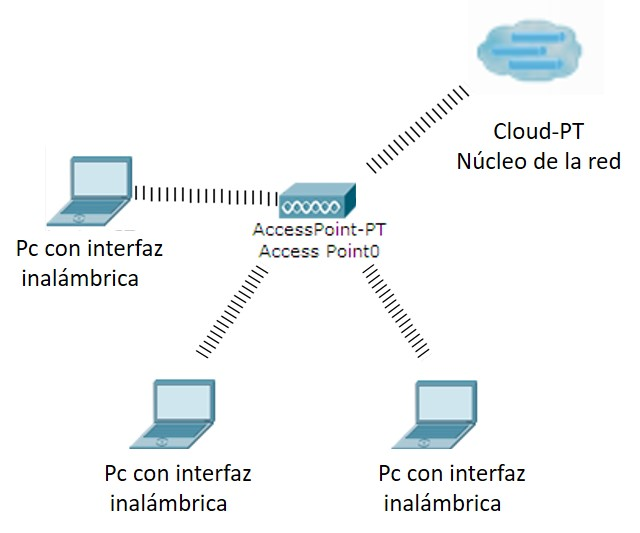
\includegraphics[width=0.5\textwidth]{marco/fig5.jpg}
\caption{Diagrama de una red Wi-Fi. }
\label{Mcinco}
\end{figure}
%

Wi-Fi es una tecnología de área local que alcanza tasas de transmisión de hasta 54 kbps en un canal de 20 MHz en la banda de 2.4 GHz (banda no licenciada) y opera con modulaciones por desplazamiento de fase, la cual es una forma de modulación angular que consiste en hacer variar la fase de la portadora entre un número de valores discretos (\cite{MT-09}). Es una plataforma bastante escalable y de fácil instalación. Sin embargo, no garantiza calidad de servicio (QoS del inglés \textit{Quality of Service} ) ni brinda mayor seguridad a la información que se transmite (\cite{MT-10}).



\paragraph{Bluetooth:}

En 1994, la compañía global de telecomunicaciones Ericsson Mobile Communications investigó la viabilidad de una interfaz de radio de baja potencia y ajo coste entre dispositivos móviles y sus accesorios, llegando a la conclusión de que dicho tipo de conexión debería ser un enlace de radio de corto alcance.\\

Esta investigación atrajo la atención de otras grandes compañías como IBM, Intel, Nokia y Toshiba, creando el SIG Bluetooth, consorcio inalámbrico que creció exponencialmente tras pocos años.\\

El nombre fue dado con motivo de honrar a un rey vikingo danés del sigo X. Haral Bluetooth, el cuál reinó desde el año 940 hasta el 985 y al que le atribuye la unificación del mencionado país y la adopción del cristianismo.\\
La relación entre el nombre y la tecnología Bluetooth es que lo que se pretende con ésta última es la unificación y armonía para permitir a diferentes dispositivos que se comuniquen a través de un estándar aceptado para la comunicación inalámbrica (\cite{MT-05}). \\

El conjunto de especificaciones Bluetooth desarrolladas por Ericsson y otras compañías responde a las necesidades de conectividad inalámbrica de corto alcance para redes ad hoc. Una red ad hoc es un tipo de red inalámbrica descentralizada, es decir, no depende de una infraestructura pre-existente. El protocolo de banda base de Bluetooth es una combinación de conmutación de circuitos y de paquetes, haciéndola idónea para transmitir tanto voz como para datos. \\

La tecnología Bluetooth se implementa en transceptores de corto alcance, de pequeño tamaño y bajo coste en dispositivos móviles, integrada de forma directa o mediante dispositivos adaptadores. La tecnología inalámbrica utiliza la banda de radio ISM mundialmente disponible de 2.4 GHz y no requiere licencia. Éstas bandas incluyen los rangos de frecuencia entre 902-928 MHz y 2.4-2.484 GHz que no requieren licencia de operador otorgada por las autoridades reguladoras de telecomunicaciones (\cite{MT-05}).\\

Los módulos de desarrollo bluetooth es un perfecto aliado para eliminar los cables en los proyectos o para conectarse a ordenadores y/o teléfonos móviles.\\

Tiene un alcance de hasta 100 metros seccionado por rangos de 10 metros, posee antena integrada, son compatibles con el resto de versiones Bluetooth, permite velocidades de transferencia de hasta 921 Kbps, y se puede conectar de forma sencilla mediante la UART(RX/TX) de cualquier micro controlador, desde donde se puede controlarlo haciendo uso de sencillos comandos AT.\\

Puede ser alimentado tanto a 5 Volts como a 3.3 Volts, y para ello dispone de un puente (jumper) de selección de la tensión de alimentación.\\

Para establecer una comunicación entre los dispositivos móviles se sigue un procedimiento para poder garantizar un cierto grado de seguridad entre los dispositivos conectados:
\begin{itemize}
\item modo pasivo,
\item solicitud, 
\item paginación,
\item descubrimiento del servicio del punto de acceso,
\item creación de un canal con el punto de acceso,
\item emparejamiento mediante el PIN(Seguridad),
\item utilización de la red.
\end{itemize}

En el modo pasivo el funcionamiento del dispositivo es normal, en la fase de Solicitud, la comunicación comienza durante la cual el principal envía una solicitud a los dispositivos que se encuentran dentro del rango, denominados los puntos de acceso, en la fase paginación el dispositivo principal elige una dirección o un punto de acceso que consta de una sincronización de su reloj y frecuencia, luego sigue la fase de descubrimiento de servicio, se establece un enlace con el punto de acceso mediante un protocolo denominado SDP (del inglés \textit{Service Discovery Protocol}), Cuando esta fase de descubrimiento de servicio finaliza, el dispositivo principal o maestro ya está listo para crear un calan de comunicación.\\

Un mecanismo de seguridad llamado emparejamiento, restringe el acceso a otros dispositivos, soló se aceptan dispositivos autorizados para brindar a la piconet cierto grado de proyección.\\

El emparejamiento se realiza mediante una clave de acceso conocida como PIN que es un Número de identificación Personal. Para esto se envía una solicitud al dispositivo de emparejamiento al dispositivo principal o maestro de tal manera que se deberá conocer la clave de acceso para llevar a cabo dicha conexión. \\
 





\paragraph{GSM}

 El Sistema Global para las comunicaciones móviles  (\cite{UPS-03}) es un sistema estándar, completamente definido para generar una comunicación entre teléfonos móviles que incorporan tecnología digital. Por ser digital cualquier usuario de GSM puede conectarse a través de su teléfono con su computadora además de poder enviar y recibir mensajes por email, faxes, navegar por internet, acceso seguro a la red informática de una compañía, así como utilizar otras funciones digitales de transmisión de datos incluyendo el servicio de mensajería cortos o mensajes de texto.\\

GSM se considera, por su velocidad de transmisión y otras características, un estándar actual de cuarta generación (4G). Una de las características principales del estándar GS es en Módulo de Identidad del Suscriptor (SIM por sus siglas en inglés). \\

La tarjeta SIM es una tarjeta inteligente desmontable que contiene la información de suscripción del usuario, parámetros de red y directorio telefónico. Esto permite al usuario mantener su información después de cambiar su teléfono. Paralelamente, el usuario también puede cambiar de operador de telefonía, manteniendo el mismo equipo, simplemente cambiando la tarjeta SIM.\\

Debido a que los mensajes SMS son recibidos prácticamente de inmediato por el destinatario y son un medio de comunicación muy personal, muchos ya los están utilizando como uno de los mejores medios para comunicación ante la sociedad.\\

\subsection{TARJETAS Y COMPONENTES ELECTRÓNICOS}

\paragraph{Arduino}

Antes de que aparecieran plataformas de hardware libre como Arduino, la creación de prototipos de sistemas \textit{software-hardware} era complejo y caro. Por ello, muchas universidades y centros de investigación empezaron a desarrollar alternativas más baratas y sencillas a finales del siglo XX. Pero estas soluciones no eran generales y su popularidad fuera de su institución era pequeña. Hasta que en 2005 nació Arduino en el instituto IVREA de Italia, como un proyecto para estudiantes dirigido por Massimo Banzi, que aplicaba los conceptos de \textit{hardware} y \textit{software} libres, lo que supuso un cambio importante (\cite{MT-01}).\\ 

El concepto de \textit{hardware} libre de Arduino hace referencia a un diseño de un sistema electrónico basado en microprocesador que está disponible de forma gratuita, para su uso o modificación. Además, el \textit{software} usado para programar el sistema es libre y de acceso gratuito, y fácil de obtener, poner en marcha y usar (\cite{MT-02}). \\

Todo esto ha hecho que los dispositivos de la plataforma Arduino (ver Figura \ref{Mtres}) se hayan popularizado y extendido enormemente, y sea posible encontrar soluciones disponibles de forma abierta, para prácticamente todo tipo de proyectos. Todos los dispositivos Arduino se programan fácilmente con el mismo entorno de desarrollo, mediante lenguaje C/C++, pudiéndose crear desde programas simples de un solo archivo basados en procedimientos, hasta programas complejos de múltiples archivos y orientados a objetos. También es fácil encontrar documentación en internet sobre cualquier aspecto de la plataforma Arduino, y hay gran cantidad de libros de texto para usuarios con distintos niveles de conocimientos (\cite{MT-03}). \\


%
\begin{figure}[H]
%\vspace{0.2cm}
\centering
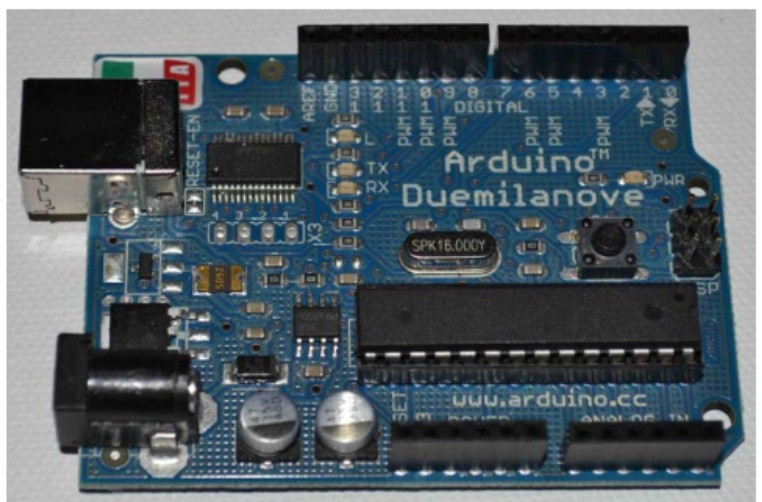
\includegraphics[width=0.5\textwidth]{marco/fig3.jpg}
\caption{Tarjeta Arduino \cite{MT-03}. }
\label{Mtres}
\end{figure}
%



\paragraph{Raspberry Pi}

La Raspberry Pi (ver Figura \ref{Mcuatro}) se comenzó a comercializar en agosto de 2011 con el objetivo de ser utilizada para incentivar el conocimiento en el uso de la electrónica y la programación en edades tempranas (\cite{MT-04}). Desde esa fecha ha transitado por 4 modelos, aumentando cada vez más su capacidad de procesamiento y prestaciones. Un modelo muy comercial es el B+, que cuenta con un procesador ARM a 700 MHz, 512 MB de memoria SDRAM (Synchronous Dynamic Random-Access Memory, en español, Memoria de Acceso Sincrónico, Dinámico y Aleatorio), salidas de video compuesto y HDMI (High-Definition Multimedia Interface, en español, Interface Multimedia de Alta Definición) hasta 1080p. Su almacenamiento es mediante tarjetas MicroSD; además posee un bajo consumo de energía llegando solamente a los 3.5 W. Además, cuenta con 40 pines de Entrada Salida de Propósito General (GPIO, del inglés \textit{General Purpose Input Output}) y el sistema operativo más usado para su operación es el Raspbian, una variante de Debían diseñada especialmente para ella.

%
\begin{figure}[H]
%\vspace{0.2cm}
\centering
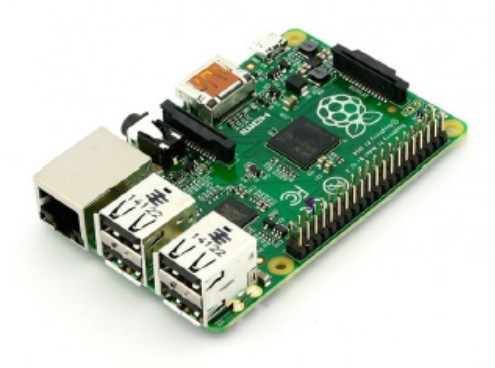
\includegraphics[width=0.5\textwidth]{marco/fig4.jpg}
\caption{Tarjeta Raspberry Pi \cite{UPS-08}. }
\label{Mcuatro}
\end{figure}
%

\paragraph{Relevador}
Un relevador es un interruptor accionado por un electroimán, un electroimán está formado por una barra de hierro dulce, llamada núcleo, rodeada por una bobina de hilo de cobre tal como se muestra en la Figura \ref{Muno}, al pasar una corriente eléctrica por la bobina el núcleo de hierro se magnetiza por efecto del campo magnético producido por la bobina, convirtiéndose en un imán tanto más potente cuanto mayor sea la intensidad de la corriente y el número de vueltas de la bobina. Al abrir de nuevo el interruptor y dejar de pasar corriente por la bobina, desaparece el campo magnético y el núcleo deja de ser un imán.

%
\begin{figure}[H]
%\vspace{0.2cm}
\centering
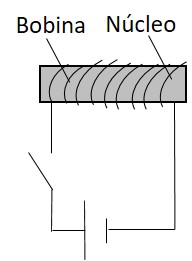
\includegraphics[width=0.4\textwidth]{marco/fig1.jpg}
\caption{Electróiman. }
\label{Muno}
\end{figure}
%

El relevador más sencillo está formado por un electroimán como el descrito anteriormente y un interruptor de contactos tal cual se muestra en la Figura \ref{Mdos}. Al pasar una pequeña corriente por la bobina, el núcleo se imanta y atrae al inducido por uno de sus extremos, empujándolo por el otro a uno de los contactos hasta que se juntan, permitiendo el paso de la corriente a través de ellos.

%
\begin{figure}[H]
%\vspace{0.2cm}
\centering
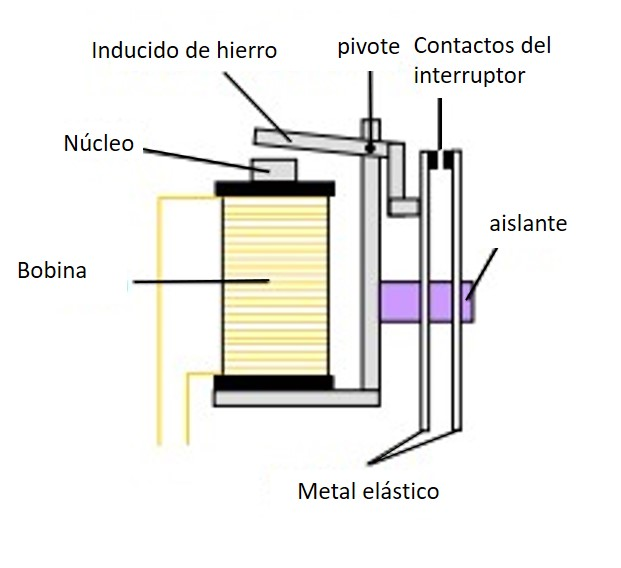
\includegraphics[width=0.5\textwidth]{marco/fig2.jpg}
\caption{Estructura del relevador. }
\label{Mdos}
\end{figure}
%

\subsection{SISTEMAS DEL VEHÍCULO}
Los sistemas principales que conforman un vehículo son el Sistema de Tracción y el Sistema de Confort. Estos están monitoreados por sensores y actuadores que apoyan la detección de fallas, además de la visualización de la información que envía el vehículo al conductor.\\

Los vehículos se clasificarán para este documento en tres principales gamas; ``gama baja", ``gama media" y ``gama alta". La clasificación de la gama depende de la seguridad y tecnología que esta implementada, entre mayor tecnología y seguridad mayor será la gama.\\


\subsection{ÁREAS DE MEJORA CONTINUA DEL VEHÍCULO}

\paragraph{GPS}

El sistema de posicionamiento global (GPS) en sus inicios comenzó como un proyecto militar hoy en día está disponible para su uso civil, operativo desde 1995 utiliza conjuntamente una red de computadora y una constelación de veinticuatro satélites para determinar por triangulación la altitud, longitud y latitud de cualquier objeto en la superficie terrestre (\cite{MT-13}).\\

El GPS es un sistema que tiene como objetivo la determinación de las coordenadas espaciales de puntos respecto de un sistema de referencia mundial. Los puntos pueden estar ubicados en cualquier lugar del planeta, pueden permanecer estáticos o en movimiento y las observaciones pueden realizarse en cualquier momento del día (\cite{MT-13}).\\

El sistema se descompone en tres segmentos básicos según Eduardo, Aldo y Gustavo mencionan en (\cite{MT-14}):

\subparagraph{Segmento espacio o espacial}

Formado por 24 satélites GPS con una órbita de 26 560 Km. De radio y un periodo de 12 horas. Cabe mencionar que a estos satélites se les incorporo la señal de una perturbación denominada SA (Selective Availability) que no es otra cosa que la disminución intencional de la precisión del sistema, también se estableció una limitación al acceso del denominado código P. Estas características fueron impuestas a los usuarios civiles por cuestiones de interés militar.


\subparagraph{Segmento control}

Consta de cinco estaciones monitoras encargadas de mantener en órbita los satélites y supervisar su correcto funcionamiento, tres antenas terrestres que envían a los satélites las señales que deben transmitir y una estación experta de supervisión de todas las operaciones.\\

Las funciones principales del segmento de control, denominado internacionalmente con las siglas OCS (del inglés \textit{Operational Control Segment}) son: monitoreo y control permanente de los satélites con el objeto de determinar y predecir las órbitas y los relojes de a bordo, la sincronización de los relojes de los satélites con el tiempo GPS y la transmisión, a cada satélite, de la información procesada.\\

El segmento control está integrado por 10 estaciones las cuales se ubican en \textit{Colorado Springs} (EUA), Isla Ascensión (Atlántico Sur), Diego García (Indico), \textit{Kwajalein} (Pacifico Occidental), \textit{Hawái} (Pacifico Oriental), Quito (Ecuador), Buenos Aires (Argentina), Hermitage (Inglaterra), \textit{Bahrain} (Golfo Pacifico), \textit{Smithfield} (Australia) como se muestra en la Figura \ref{Mseis}.


%
\begin{figure}[H]
%\vspace{0.2cm}
\centering
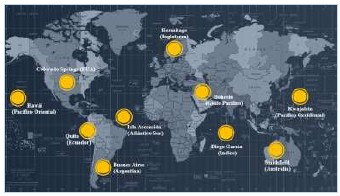
\includegraphics[width=0.5\textwidth]{marco/fig7.jpg}
\caption{Segmento control GPS.}
\label{Mseis}
\end{figure}
%


\subparagraph{Segmento usuario}
Está constituido por los instrumentos utilizados para la recepción y procesamiento de la señal emitida por los satélites, formado por las antenas y los receptores pasivos situados en tierra. La antena está conectada por cable al receptor o en otros casos forman una sola unidad.\\

Las coordenadas que se calculan corresponden al centro radioeléctrico de la antena. El receptor consta de un mínimo de 4 canales (generalmente 10 o 12) que permiten recibir y procesar simultáneamente la señal de cada satélite. Posee además un oscilador de cuarzo que permite generar la frecuencia de referencia para realizar la observación. \\

Un microprocesador interno con el \textit{software} correspondiente calcula las coordenadas de la antena y la velocidad y acimut si el aparato está en movimiento.\\

Las características que posee el sistema GPS son las siguientes:
\begin{itemize}
\item Compuesto por 24 satélites.
\item Los satélites se ubican en 6 órbitas planas prácticamente circulares, con inclinación de 55º respecto al plano del Ecuador y con una distribución aproximadamente uniforme; con 4 satélites en cada órbita.
\item Se encuentran aproximadamente a 20, 180 km de altura.
\item Tienen 12 h. de período de rotación (en tiempo sidéreo) u 11 h. 58 min. (en tiempo oficial).
\item También hay satélites en órbita que se encuentran desactivados y disponibles como reemplazo.
\item Con la constelación completa, se dispone, en cualquier punto y momento, entre 5 y 11 satélites observables, con geometría favorable.
\item El tiempo máximo de observación de un satélite es de hasta 4 horas 15 minutos.
\end{itemize}

\paragraph{Seguridad Vehícular}

La seguridad vehicular es el conjunto de elementos y sistemas ubicados en el automotor para que el usuario se encuentre protegido de todo daño o riesgo en caso de un accidente de tránsito. Estos dispositivos dotan a los vehículos de los más altos niveles de seguridad y de mejores condiciones para una conducción adecuada.

La principal misión de la seguridad vehicular es la de proteger la integridad física y psicológica del conductor y de los ocupantes, antes y en el momento que se provoque el accidente, por medio de la reducción de los riesgos y la limitación de las consecuencias del impacto.

El objetivo principal de este sistema es disminuir el riesgo de accidentes que se pueden producir durante el uso regular y habitual del vehículo, por lo cual los dispositivos y elementos que lo conforman deben garantizar que el conductor no sufra perturbaciones en la marcha del vehículo y además que se facilite la manipulación de los mandos que permiten que éste pueda funcionar.

De acuerdo a la funcionabilidad de los diferentes dispositivos y elementos que conforman este sistema, se puede clasificar (\cite{MT-15}):
\begin{itemize}
	\item Seguridad de marcha: Tiene como objetivo garantizar el correcto funcionamiento dinámico del vehículo en los mecanismos de dirección, frenos, suspensión y conjuntos de trasmisión de las ruedas.

	\item Sistema en la percepción de señales: Se determina por el buen estado y aplicación de los dispositivos de iluminación, dispositivos acústicos de advertencia y medidas de visión.

	\item Seguridad de servicio: Establece la facilidad que brinda el vehículo para poder manipular los mandos y controles durante la conducción de manera confortable
\end{itemize}
Por otra parte, el sistema de seguridad pasivo tiene la finalidad de disminuir las consecuencias posteriores a un accidente, para esto se debe tener en cuenta el comportamiento de la estructura del vehículo en el momento del impacto y luego del mismo, además de la utilización de mecanismos y elementos que detengan o disminuyan la evolución del accidente.\\
\begin{itemize}
	\item
Seguridad interior: Tiene como objetivo precautelar el estado de supervivencia de los ocupantes del vehículo cuando se provoca un accidente buscando reducir el impacto y facilitando la liberación de los accidentados.\\
\end{itemize}

Dentro de las medidas de protección se tiene el comportamiento de la deformación de la carrocería en el habitáculo, sistemas de sujeción, fijación de parabrisas, elementos de protección, etc.\\
\begin{itemize}
	\item
Seguridad exterior: Busca reducir las lesiones de las personas que al estar involucradas en el accidente no son ocupantes del vehículo, por lo que en este caso influye el comportamiento de la carrocería ante el impacto y la forma exterior que tiene la misma.\\
\end{itemize}
Dentro de las medidas de seguridad se debe considerar la disposición y aplicación de elementos como faros, limpiaparabrisas, manecillas, etc. (\cite{MT-15}).


\paragraph{Sistema de iluminación del vehículo}

El sistema de iluminación, clave en la seguridad activa de un vehículo, proporciona la cantidad adecuada de luz para la correcta conducción del automotor en diferentes situaciones adversas de visibilidad; a través de dispositivos lumínicos tales como luces incandescentes, leds, faros, neón, halógeno, ver Figura \ref{Mcinco2}, que en conjunto y en una distribución adecuada sirven de localización, información y advertencia de acciones ejecutadas por el conductor.\\

Normas internacionales de calor de luz ayudan a interpretar de mejor manera la funcionalidad de cada dispositivo lumínico; faros traseros de color rojo, laterales o direccionales color ámbar y faros delanteros color amarillo o blanco.

De acuerdo a la ubicación de los dispositivos lumínicos, podemos dividir el sistema de iluminación en tres grupos:
\begin{itemize}
	\item
	Faros y luces auxiliares de iluminación delantera.
    	\item
	Faros frontales, laterales y traseros de señalización.
    	\item
	Luz interior y otros dispositivos lumínicos.
\end{itemize}
%
\begin{figure}[H]
%\vspace{0.2cm}
\centering
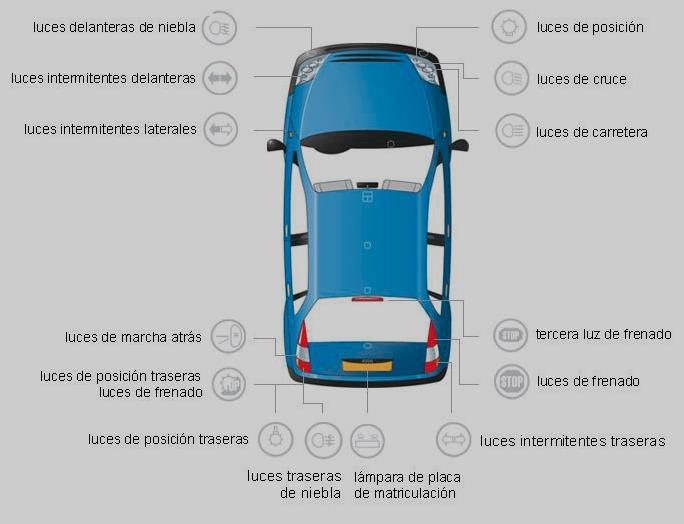
\includegraphics[width=0.5\textwidth]{marco/fig6.jpg}
\caption{Sistema de iluminación general de un vehículo.}
\label{Mcinco2}
\end{figure}
%

\paragraph{Sistema de alarma de seguridad}

Un sistema de alarma es un elemento de seguridad activa que permite advertir al conductor de situaciones anormales en el vehículo, y ejecutar una acción rápida de acuerdo al problema presente. 

En la actualidad la mayoría de las alarmas modernas están constituidas por distintos tipos de sensores, interruptores, sirenas, receptor de radio para control inalámbrico, batería auxiliar de alimentación del sistema de alarma y una unidad central de monitoreo.

De acuerdo a la tecnología utilizada y al propósito del sistema de alarma, se puede distinguir un sistema antirrobo y un sistema de seguridad centralizado.

\textbf{Sistema Antirrobo:}
Es la forma básica de un sistema de alarma, formada por una centralita que gestionara el activar de todos los interruptores, sensores, dispositivos sonoros del vehículo; además de un mecanismo traba volante y corta corriente.

\textbf{Sistema de seguridad centralizado:}
Cumple la función principal de todo sistema de alarma convencional y adicionalmente bloquea el vehículo en su totalidad, impidiendo apertura desde el interior y exterior. Utiliza tecnología más sofisticada con una unidad central que puede desconectar si es necesario el computador o cerebro del automotor. 

Distintas tecnologías aplicadas como GPS utilizada para la localización exacta a través de un centro de operaciones; una alarma silenciosa que lleva un registro celular que informa vía SMS de la situación actual el vehículo; un sistema Keyless para el encendido electrónico sin la necesidad de utilizar llaves. 

Vehículos de nueva generación incorporan sistemas biométricos en sus unidades aprovechando las características únicas que estos ofrecen como son lectores de retina, huella dactilar, reconocimiento facial, reconocimiento de voz
 \cite{MT-16}.



\clearpage
\section{METODOLOGÍA}
En el presente capítulo se muestra el procedimiento que se desarrollo para la elaboración de la metodología que se propone, basado en las actividades previas y la descripción de los pasos a seguir, manipulando y monitoreando la informacíon de sensores y actuadores mediante el dispositivo móvil.

\subsection{ESTRUCTURA GENERAL}

Se presenta una estructura general de comunicación donde se incluye un bosquejo del flujo de la comunicación entre los actuadores y sensores utilizados hasta el dispositivo móvil. esta propuesta se divide en 5 fases principales: i) Aplicación móvil, ii) Conectividad, iii) Tarjeta electrónica, iv) Circuito de potencia y v) Actuadores y sensores.

%
\begin{figure}[H]
%\vspace{0.2cm}
\centering
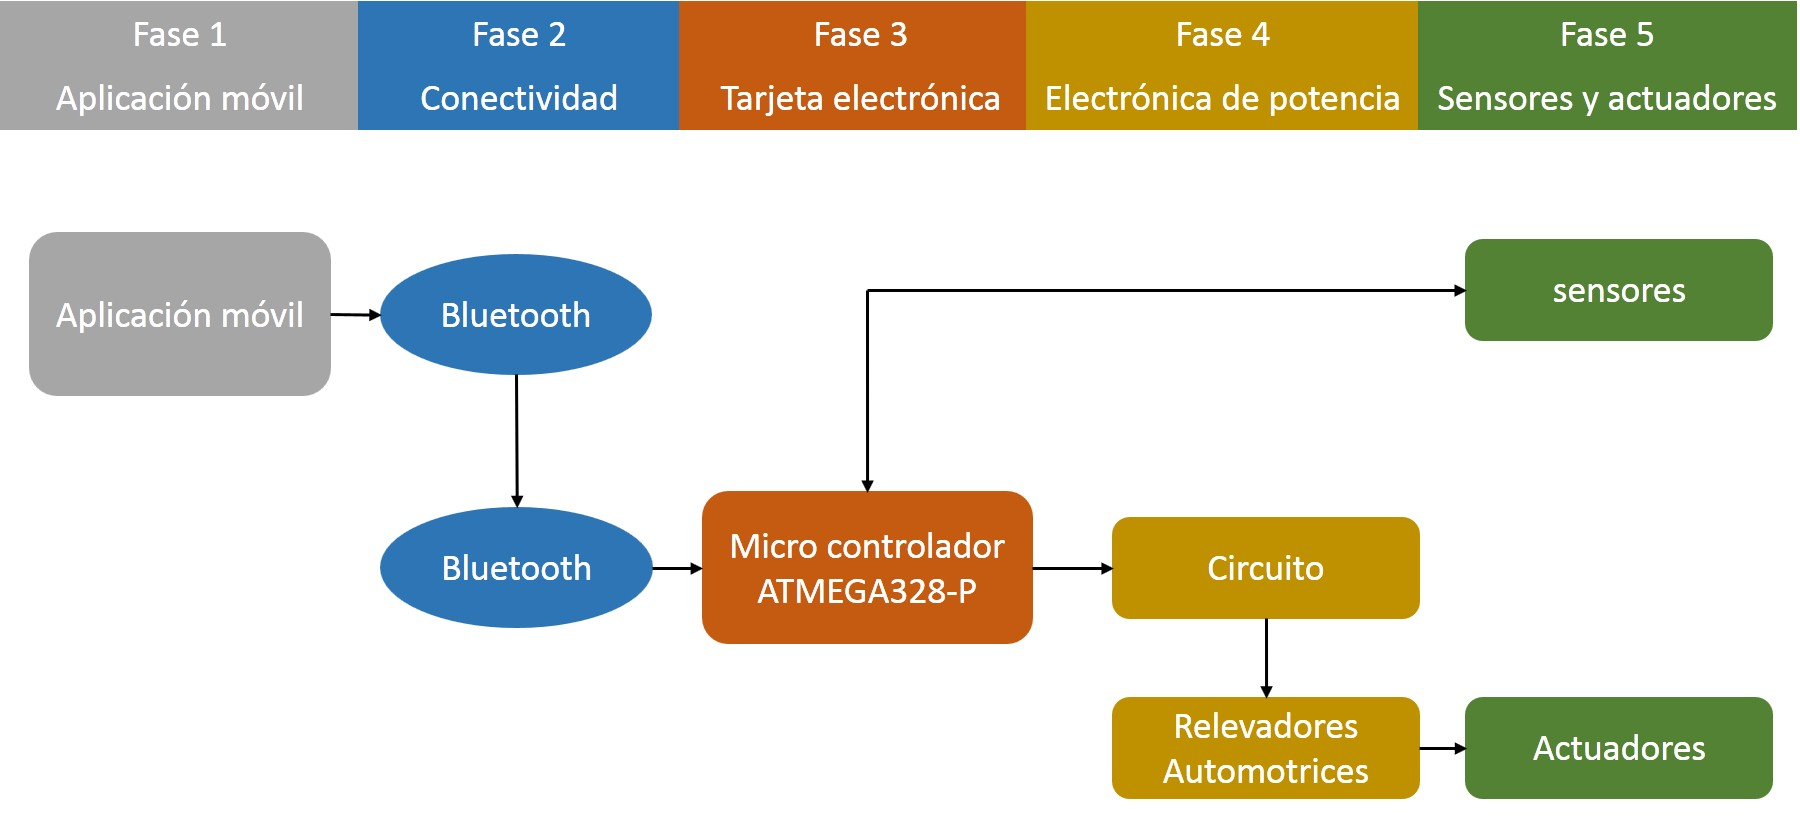
\includegraphics[width=0.95\textwidth]{metodologia/fig_1.jpg}
\caption{Estructura general de comunicación}
\label{Meuno}
\end{figure}
%

 
 Tal como se muestra en la Figura \ref{Meuno} el proceso de manipulación y monitoreo se describe en la siguiente lista.
 \begin{enumerate}
\item La aplicación móvil se inicia y envia comandos.
\item Los comandos son enviados a través de la comunicación inalámbrica Bluetooth.
\item La placa electrónica recibe los datos por medio del Bluetooth y regresa una repuesta.
\item Según los datos activa o desactiva ciertas señales que encienden o apagan un relevador por medio del circuito de potencia.
\item El relevador transmite o evita el paso de la señal \textit{Low} hacia el actuador.
\item El actuador se activa o desactiva segun la transmisión del relevador.

\end{enumerate}


\subsection{APLICACION MÓVIL}

La aplicación móvil se desarrolló por medio de la plataforma Android Studio\textregistered enfocada al sistema operativo Android, los requisitos mínimos de \textit{software} para que el paquete de aplicaciones Android (APK del inglés \textit{Android Application Package}) funcione de manera correcta es necesario tener una versión mínima de Android 3.0. La estructura general de la aplicación móvil se muestra en la Figura \ref{Mestrucgeral}.\\

%
\begin{figure}[H]
%\vspace{0.2cm}
\centering
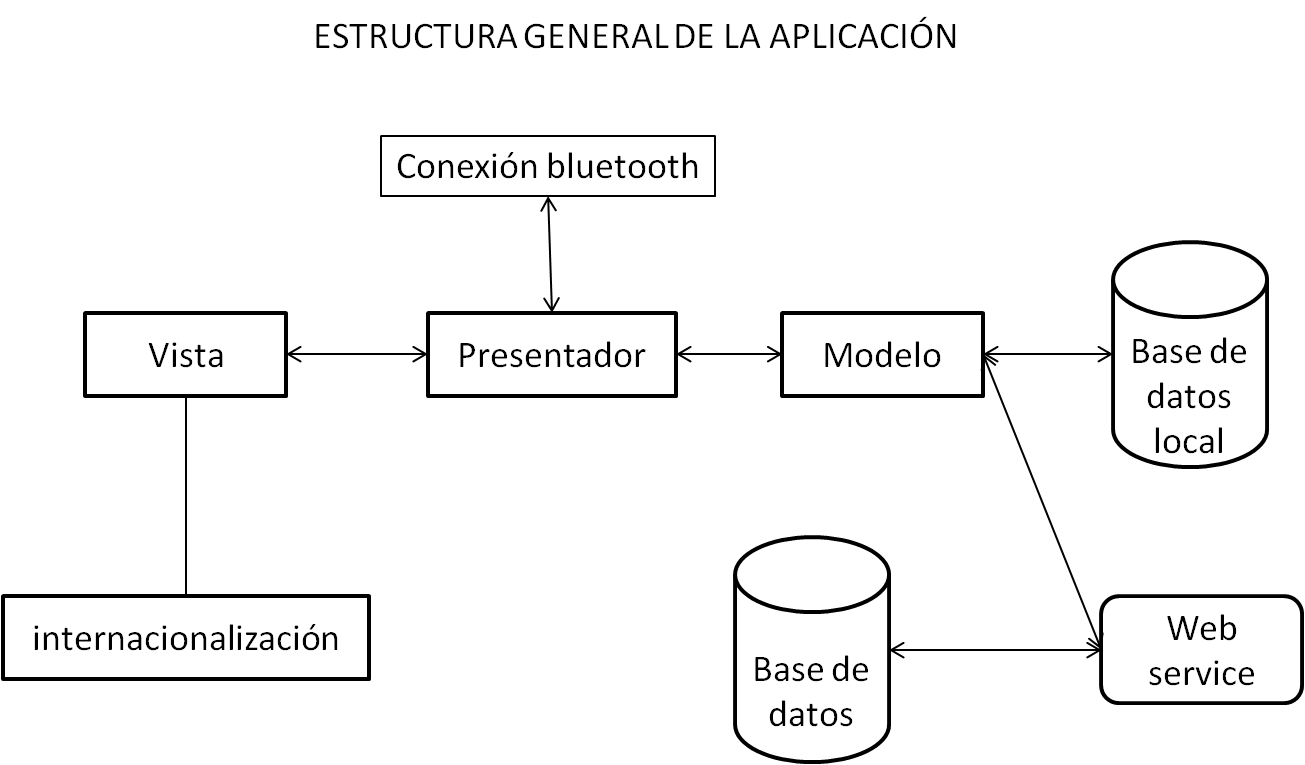
\includegraphics[width=0.95\textwidth]{metodologia/fig1.png}
\caption{Estructura general de la aplicación.}
\label{Mestrucgeral}
\end{figure}
%


La aplicación se desarrollo siguiendo un patrón de arquitectura Modelo-Vista-Presentador, debido a la relación de diseño, actividad y datos, usado comunmente en la construcción de interfaces de usuario. Este patrón permite una escalabilidad sencilla y una estructura independiente para cada capa, permitiendo realizar modificaciones de una forma muy fácil a la capa seleccionada.\\

La capa de presentación esta programada para actuar como intermediario entre la vista y el modelo.  Se encarga de tomar acciones mediante las reglas de negocio cuando el usuario interactua con la vista y recupera los datos del modelo enviandolos en formato necesario para la vista. En la capa vista se diseño toda la interfaz para el usuario y su unica funcionalidad es llamar a un método de la capa presentación cada vez que hay una acción en la interfaz. Y finalmente en la capa de modelo se recuperan los datos y se hace la conexión con un servicio Web y una base de datos donde se consulta la información mediante procedimientos almacenados.\\

La aplicación cuenta con la internacionalización, una práctica de diseño y desarrollo que facilita la migración del contenido en el futuro, ya que eliminar obstáculos a la localización o la distribución internacional. Permitiendo modificar el idioma de la vista de manera sencilla al almacenar todos los textos en variables y ubicarlos en un solo archivo.\\

Se diseño el diagrama de clases de la aplicación móvil tal cual se muestra en la Figura \ref{diaclas}, existen 5 clases de entidades en el diagrama. 
%
\begin{figure}[H]
%\vspace{0.2cm}
\centering
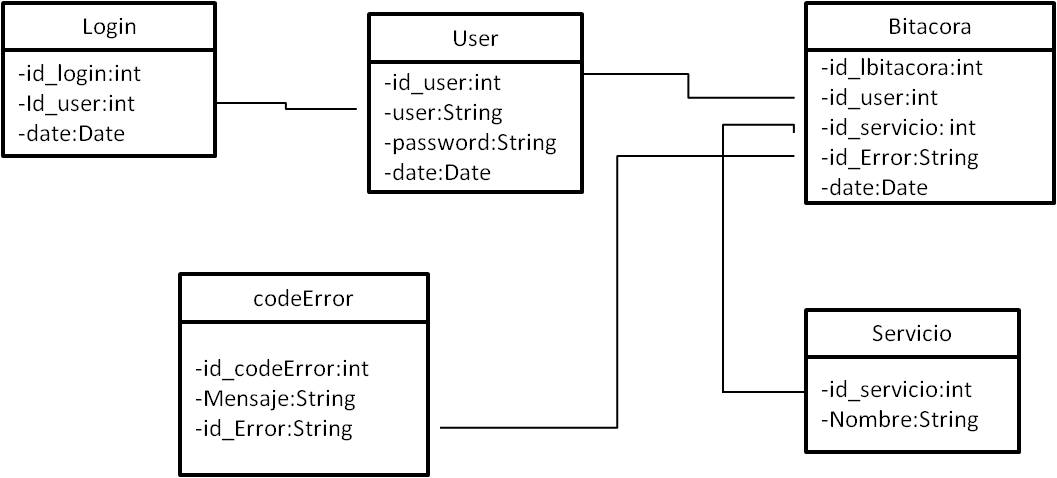
\includegraphics[width=0.95\textwidth]{metodologia/DClases.jpg}
\caption{Diagrama de clases de la aplicación móvil.}
\label{diaclas}
\end{figure}
%
\begin{enumerate}
\item  clase \textit{Login}: esta entidad representa el historial de acceso a la aplicación, el usuario cada vez que accede la aplicación se registra en la base de datos. Los atributos incluidos de la clase \textit{login} son idlogin, iduser, date.
\item clase \textit{User}: esta entidad representa el acceso a la aplicación, cada vez que el usuario accede se tiene que revisar la base de datos con la información ingresada. Los atributos includos de la clase \textit{User} son iduser, user, password, date.
\item clase \textit{codeError}: esta entidad representa los codigos de posibles errores, cuando existe un error se muestra un mensaje en la aplicación sobre el error en la base de datos al guardar o extraer algún dato. Los atributos incluidos de la clase \textit{codeError} son idcode, Mensaje, iderror.
\item clase \textit{service}: esta entidad representa los servicios que se pueden realizar por ejemplo encender el vehículo, subir los vidrios, entre otros.Esta información se utiliza para guardar el historial de servicios. Los atributos incluidos de la clase \textit{service} son idservicio, nombre.
\item clase \textit{bitacora}: esta entidad representa el historial de servicios que se han realizado en la aplicación. Los atributos incluidos de la clase \textit{bitacora} son idbitacora, iduser, idservice, iderror, date.
\end{enumerate}
Los diagramas de secuencia describen el funcionamiento del proceso y como se ha pasado el mensaje en una secuencia temporal, la información se envia a través de parametros mediante un objecto de transferencia de datos, cuya responsabilidad es almacenar y entregar sus propios datos entre las diferentes capas. La Figura \ref{ds1} describe la secuencia de eventos para iniciar sesión.

%
\begin{figure}[H]
%\vspace{0.2cm}
\centering
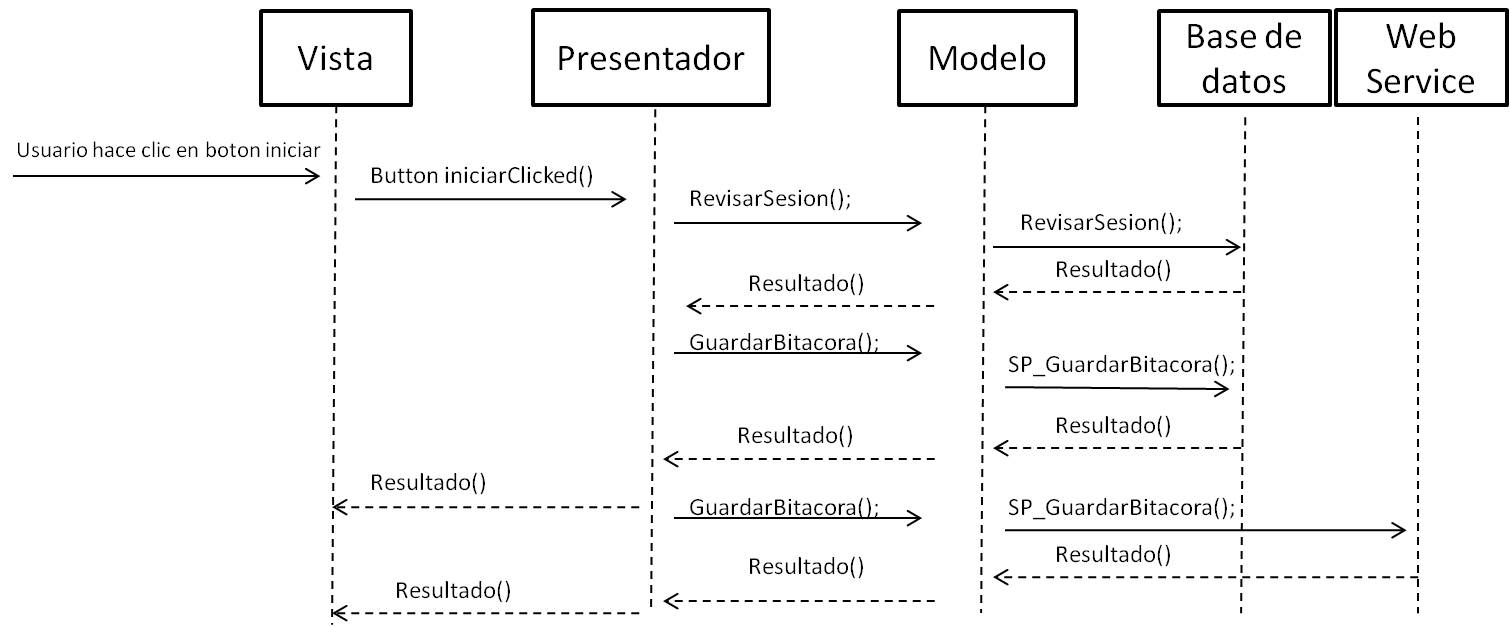
\includegraphics[width=0.95\textwidth]{metodologia/DSIniciarSesion.jpg}
\caption{Diagrama de secuencia del flujo de inicio de sesión.}
\label{ds1}
\end{figure}
%

 \begin{enumerate}
\item El usuario inicia la aplicación, inserta su usuario y su contraseña después al oprimir el boton iniciar se pasa a la capa de presentador.
\item La capa de presentador toma los datos del usuario y la contraseña y los envia a través de la capa modelo hacia la base de datos local, verificando que coincidan los datos.
\item La base de datos regresa una respuesta a la capa de modelo y regresa el resultado a la capa presentador.
\item La capa presentador revisa el resultado según las reglas de negocio establecidas y dependiendo del dato cambia la vista o manda un mensaje de error.
\item La capa presentador envia una petición de guardado hacia la base de datos para el registro de las actividades en la aplicación formando un historial, al igual que envia la información de la bitacora hacia el servicio web para crear un registro de la aplicación en linea.
\end{enumerate}

La Figura \ref{ds2} se muestra el evento de la secuencia del inicio del Bluetooth
%
\begin{figure}[H]
%\vspace{0.2cm}
\centering
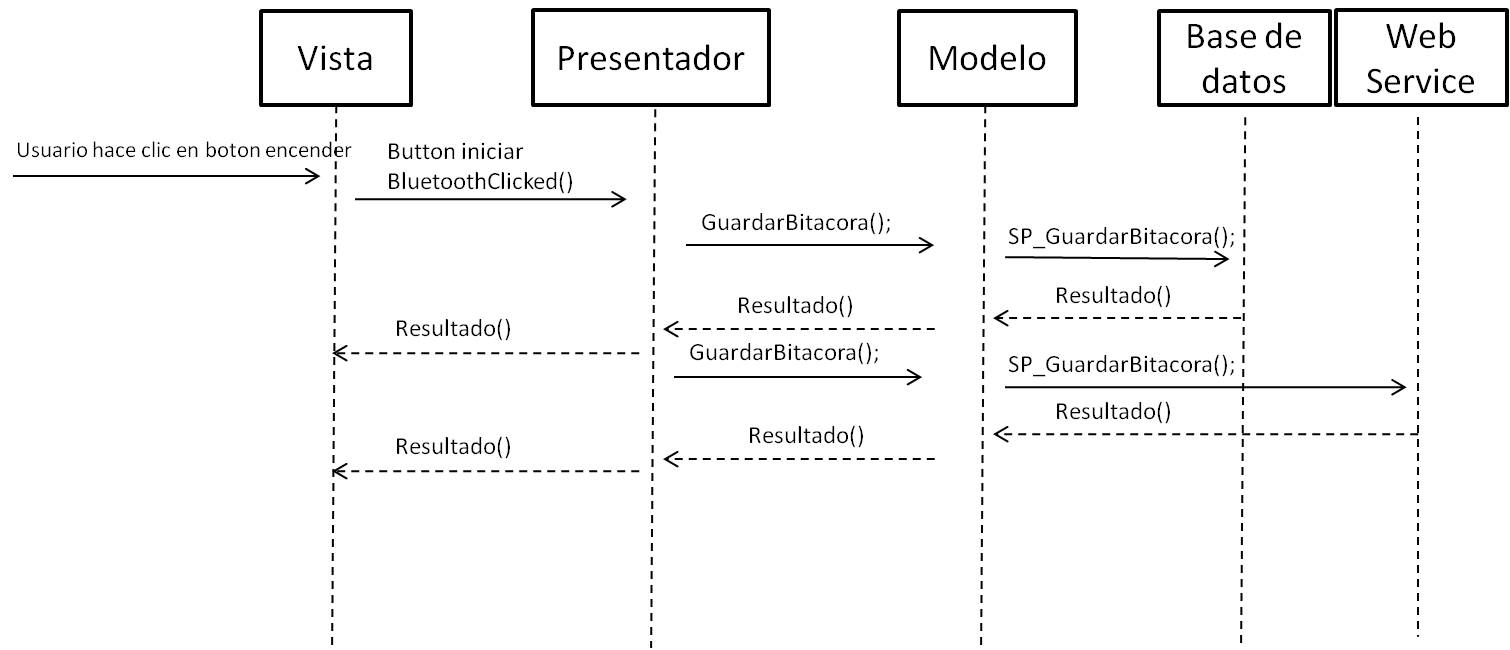
\includegraphics[width=0.95\textwidth]{metodologia/DSIniciarBluetooth.jpg}
\caption{Diagrama de secuencia del flujo de inicio del Bluetooth.}
\label{ds2}
\end{figure}


 \begin{enumerate}
\item El usuario preciona el boton para activar la conexión del Bluetooth.
\item La capa de presentador ejecuta la acción de encender la señal del Bluetooth.
\item{La capa presentador envia a la capa vista la información necesaria para cambiar de pantalla o enviar un mensaje de error}.
\item La capa presentador envia una petición de guardado hacia la base de datos para el registro de las actividades en la aplicación formando un historial, al igual que envia la información de la bitacora hacia el servicio web para crear un registro de la aplicación en linea.
\end{enumerate}

La Figura \ref{ds3} se muestra el evento de la secuencia del menu de opciones de la aplicación.
%
\begin{figure}[H]
%\vspace{0.2cm}
\centering
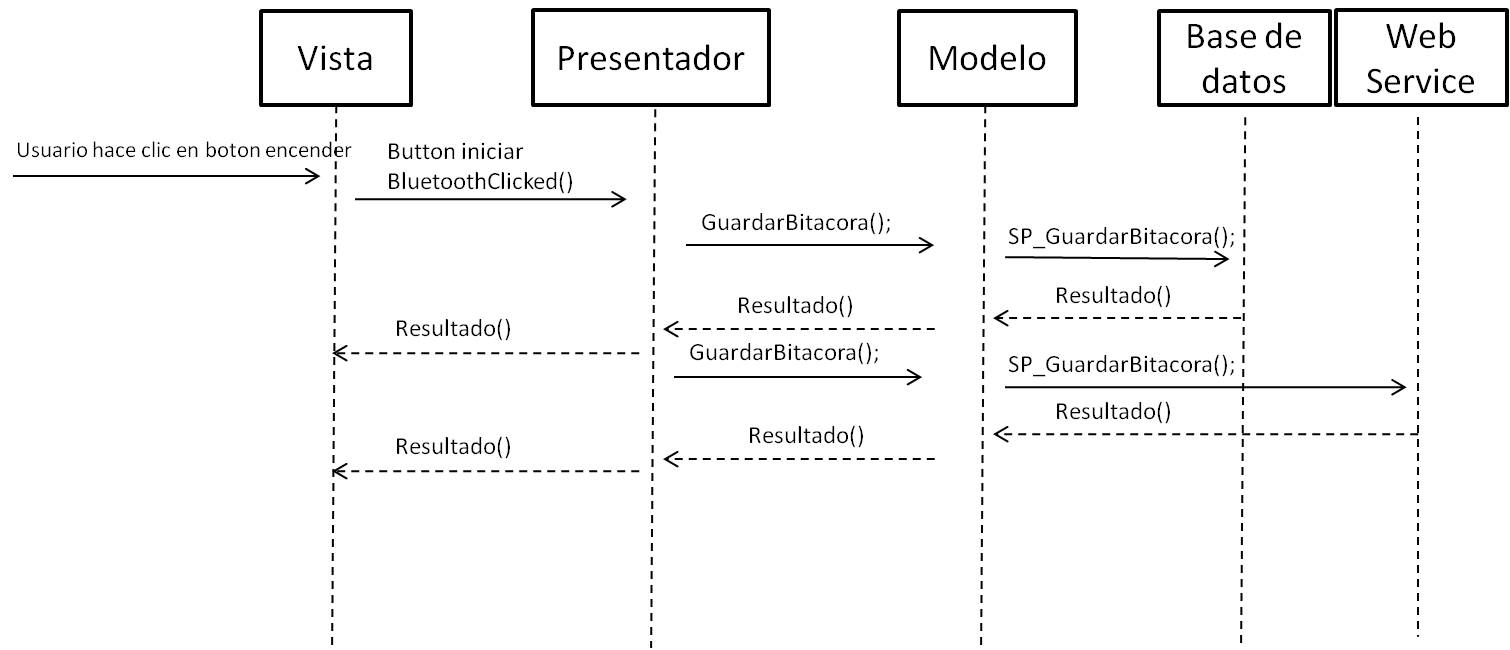
\includegraphics[width=0.95\textwidth]{metodologia/DSIniciarBluetooth.jpg}
\caption{Diagrama de secuencia del flujo del menu de opciones de la aplicación.}
\label{ds3}
\end{figure}
%

 \begin{enumerate}
\item El usuario selecciona una opción del menu.
\item La capa de presentador toma la información de la opción seleccionada y regresa a la vista la nueva pantalla o un mensaje de error.
\item La capa presentador envia una petición de guardado hacia la base de datos para el registro de las actividades en la aplicación formando un historial, al igual que envia la información de la bitacora hacia el servicio web para crear un registro de la aplicación en linea.
\end{enumerate}

La Figura \ref{ds4} se muestra el evento de la secuencia de subir el vidrio.\\
\begin{figure}[H]
%\vspace{0.2cm}
\centering
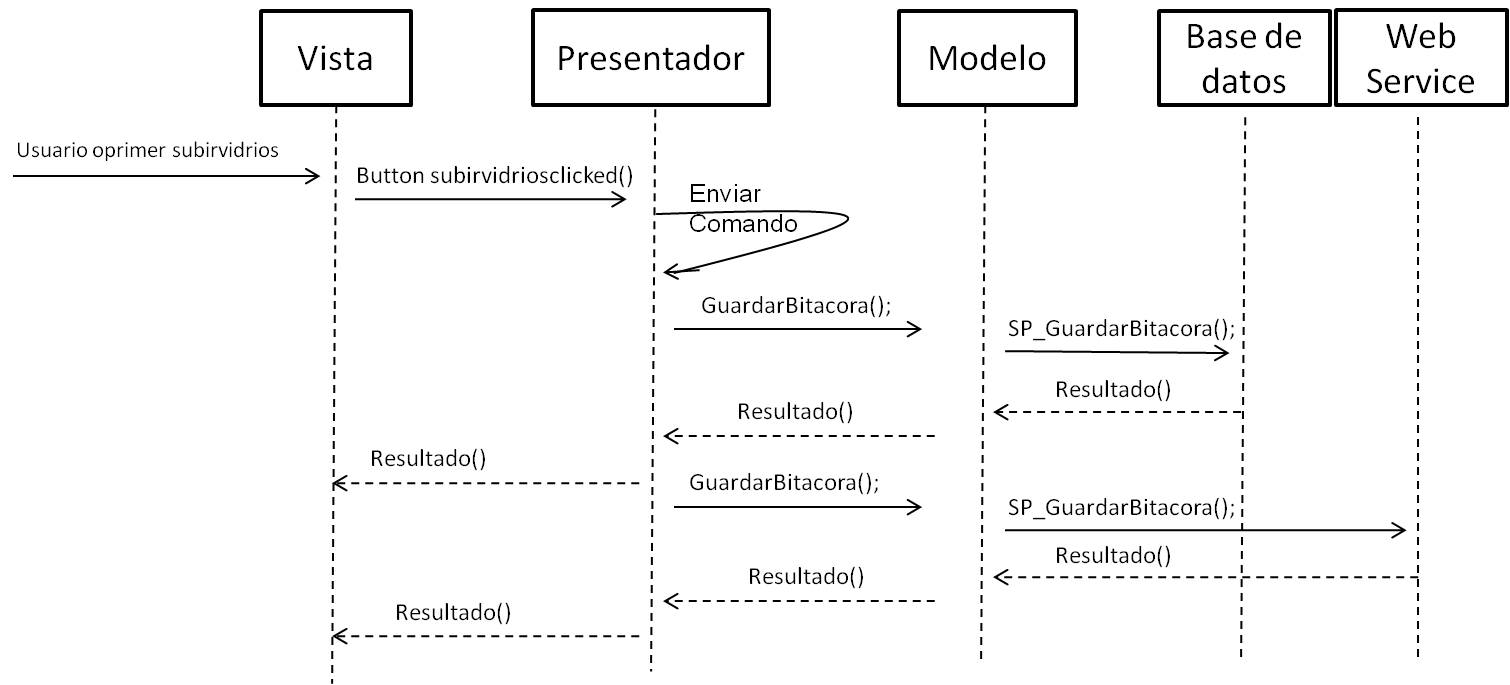
\includegraphics[width=0.95\textwidth]{metodologia/DSSubirVidrios.jpg}
\caption{Diagrama de secuencia del flujo de la funcionalidad subir vidrios.}
\label{ds4}
\end{figure}
%
 \begin{enumerate}
\item El usuario selecciona la opción de subir vidrios.
\item La capa de presentador toma la información de la opción seleccionada y la envia via Bluetooth a la tarjeta electrónica y espera una respuesta de la tarjeta electrónica por el mismo medio de comunicación.
\item Después de adquirir la respuesta envia a la pantalla un mensaje.
\item La capa presentador envia una petición de guardado hacia la base de datos para el registro de las actividades en la aplicación formando un historial, al igual que envia la información de la bitacora hacia el servicio web para crear un registro de la aplicación en linea.
\end{enumerate}

La Figura \ref{ds5} se muestra el evento de la secuencia de bajar el vidrio.\\
\begin{figure}[H]
%\vspace{0.2cm}
\centering
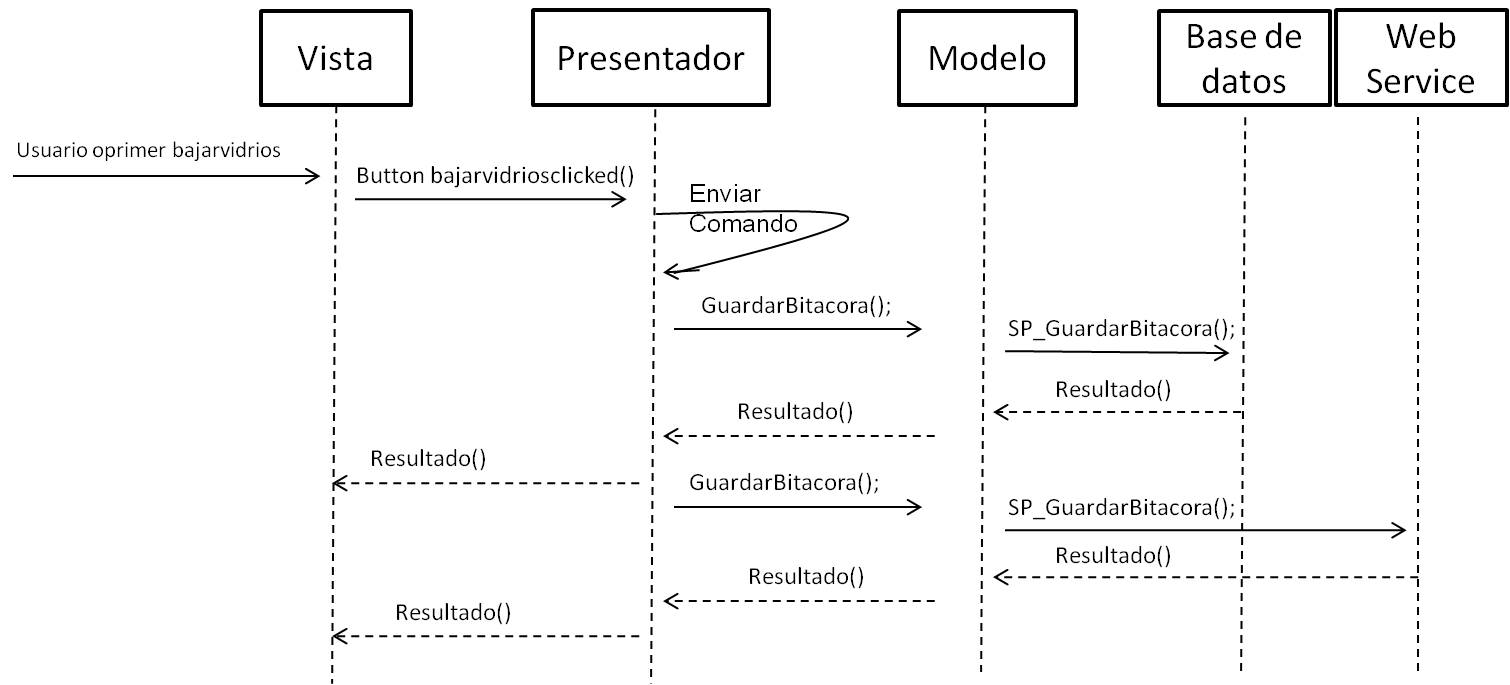
\includegraphics[width=0.95\textwidth]{metodologia/DSbajarvidrios.jpg}
\caption{Diagrama de secuencia del flujode la funcionalidad bajar vidrios.}
\label{ds5}
\end{figure}
%
 \begin{enumerate}
\item El usuario selecciona la opción de bajar vidrios.
\item La capa de presentador toma la información de la opción seleccionada y la envia via Bluetooth a la tarjeta electrónica y espera una respuesta de la tarjeta electrónica por el mismo medio de comunicación.
\item Después de adquirir la respuesta envia a la pantalla un mensaje.
\item La capa presentador envia una petición de guardado hacia la base de datos para el registro de las actividades en la aplicación formando un historial, al igual que envia la información de la bitacora hacia el servicio web para crear un registro de la aplicación en linea.
\end{enumerate}

La Figura \ref{ds6} se muestra el evento de la secuencia de poner seguro a las puertas.\\
\begin{figure}[H]
%\vspace{0.2cm}
\centering
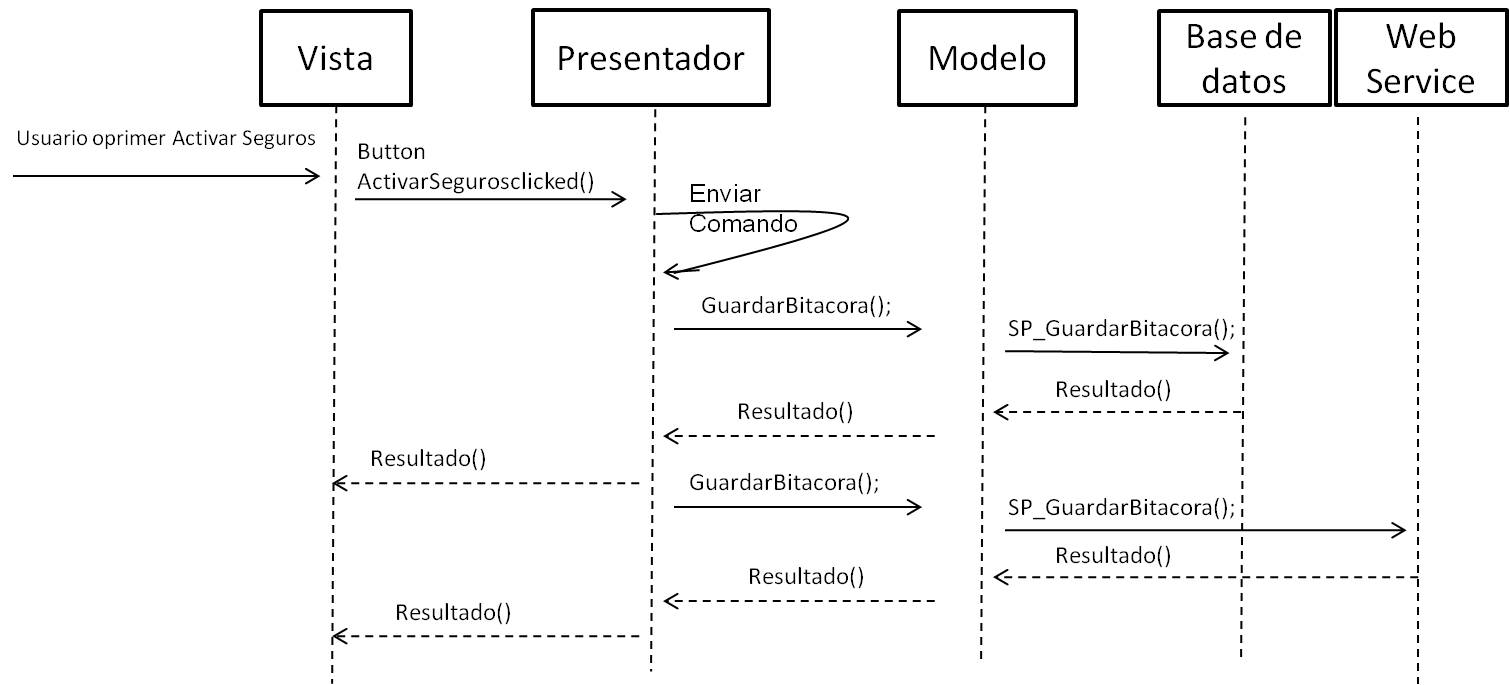
\includegraphics[width=0.95\textwidth]{metodologia/DSActivarSeguros.jpg}
\caption{Diagrama de secuencia del flujo de la funcionalidad activar seguros.}
\label{ds6}
\end{figure}
%
 \begin{enumerate}
\item El usuario selecciona la opción de poner seguro en las puertas.
\item La capa de presentador toma la información de la opción seleccionada y la envia via Bluetooth a la tarjeta electrónica y espera una respuesta de la tarjeta electrónica por el mismo medio de comunicación.
\item Después de adquirir la respuesta envia a la pantalla un mensaje.
\item La capa presentador envia una petición de guardado hacia la base de datos para el registro de las actividades en la aplicación formando un historial, al igual que envia la información de la bitacora hacia el servicio web para crear un registro de la aplicación en linea.
\end{enumerate}

La Figura \ref{ds7} se muestra el evento de la secuencia de quitar el seguro de las puertas.\\
\begin{figure}[H]
%\vspace{0.2cm}
\centering
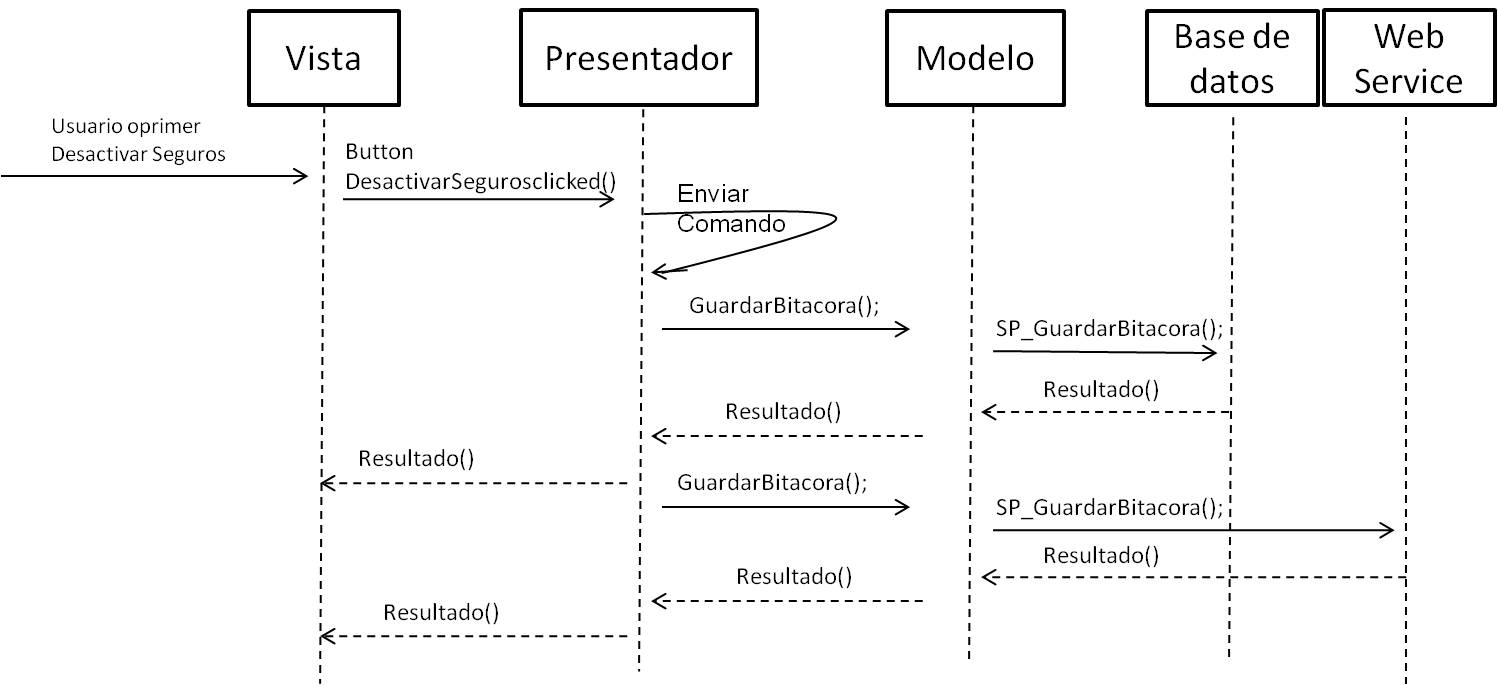
\includegraphics[width=0.95\textwidth]{metodologia/DSDesactivarSeguros.jpg}
\caption{Diagrama de secuencia del flujo de la funcionalidad desactivar seguros.}
\label{ds7}
\end{figure}
%
 \begin{enumerate}
\item El usuario selecciona la opción de quitar seguro en las puertas.
\item La capa de presentador toma la información de la opción seleccionada y la envia via Bluetooth a la tarjeta electrónica y espera una respuesta de la tarjeta electrónica por el mismo medio de comunicación.
\item Después de adquirir la respuesta envia a la pantalla un mensaje.
\item La capa presentador envia una petición de guardado hacia la base de datos para el registro de las actividades en la aplicación formando un historial, al igual que envia la información de la bitacora hacia el servicio web para crear un registro de la aplicación en linea.
\end{enumerate}

La Figura \ref{ds8} se muestra el evento de la secuencia de activar o desactivar las luces interiores.\\
\begin{figure}[H]
%\vspace{0.2cm}
\centering
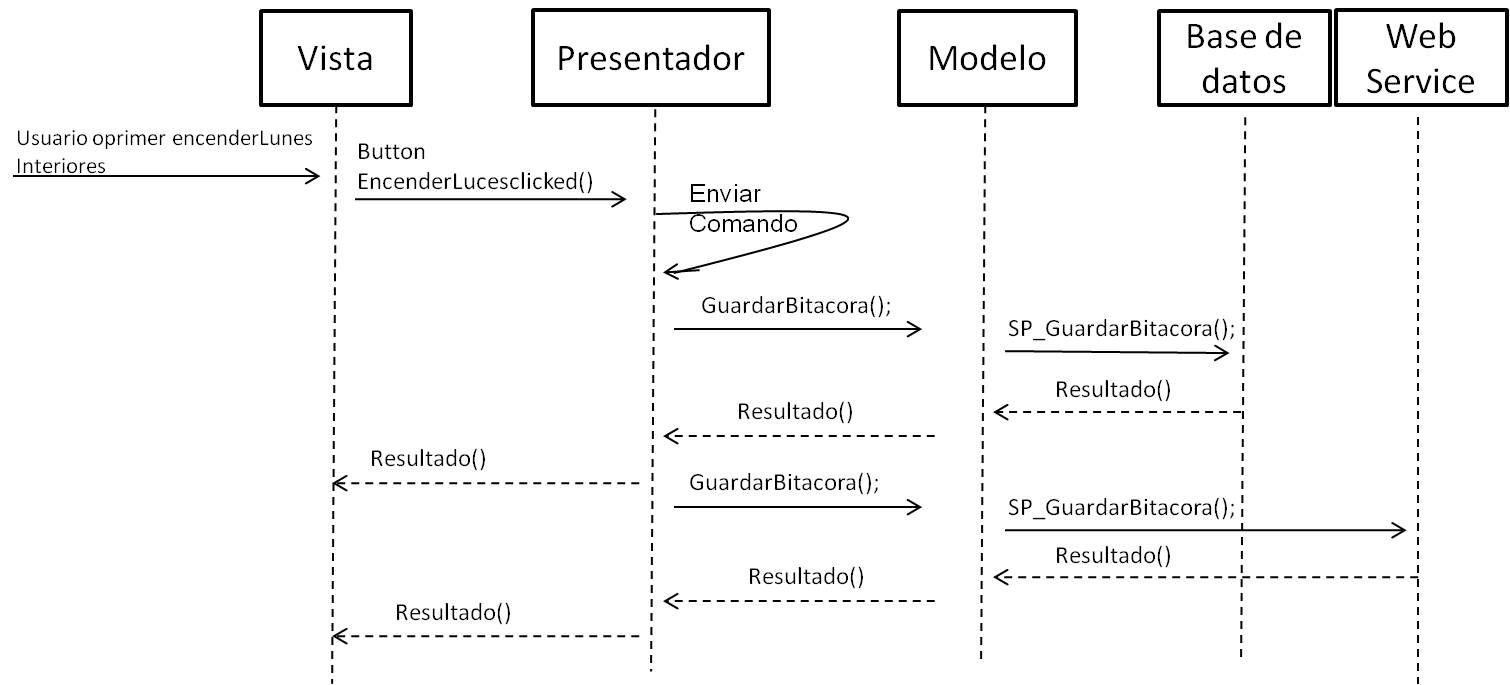
\includegraphics[width=0.95\textwidth]{metodologia/DSEncenderLucesInteriores.jpg}
\caption{Diagrama de secuencia del flujode la funcionalidad encender/apgar luces interiores.}
\label{ds8}
\end{figure}
%
 \begin{enumerate}
\item El usuario selecciona la opción de luces interiores.
\item La capa de presentador toma la información de la opción seleccionada y la envia via Bluetooth a la tarjeta electrónica y espera una respuesta de la tarjeta electrónica por el mismo medio de comunicación.
\item Después de adquirir la respuesta envia a la pantalla un mensaje.
\item La capa presentador envia una petición de guardado hacia la base de datos para el registro de las actividades en la aplicación formando un historial, al igual que envia la información de la bitacora hacia el servicio web para crear un registro de la aplicación en linea.
\end{enumerate}

La Figura \ref{ds9} se muestra el evento de la secuencia de activar o desactivar las luces exteriores.\\
\begin{figure}[H]
%\vspace{0.2cm}
\centering
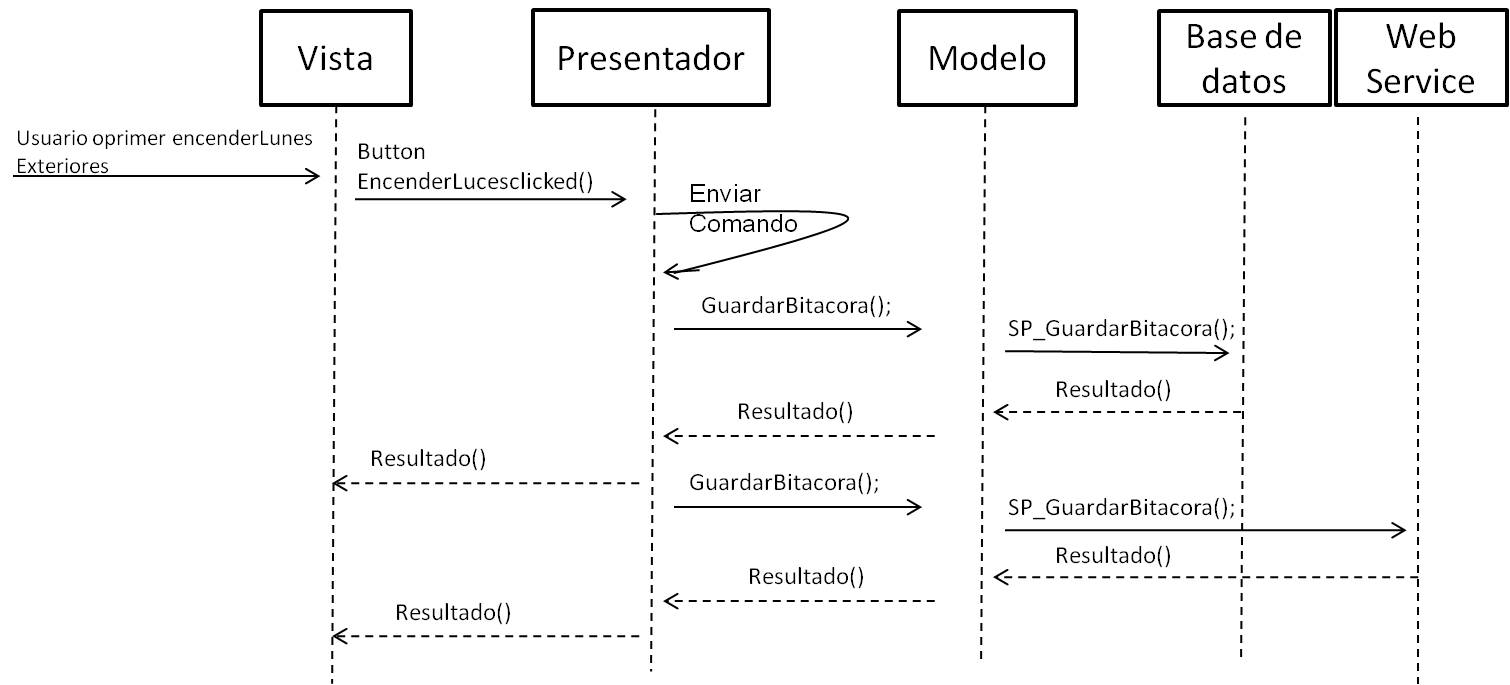
\includegraphics[width=0.95\textwidth]{metodologia/DSEncenderLucesExteriores.jpg}
\caption{Diagrama de secuencia del flujo de la funcionalidad encender/apagar luces exteriores.}
\label{ds9}
\end{figure}
%
 \begin{enumerate}
\item El usuario selecciona la opción de luces exteriores.
\item La capa de presentador toma la información de la opción seleccionada y la envia via Bluetooth a la tarjeta electrónica y espera una respuesta de la tarjeta electrónica por el mismo medio de comunicación.
\item Después de adquirir la respuesta envia a la pantalla un mensaje.
\item La capa presentador envia una petición de guardado hacia la base de datos para el registro de las actividades en la aplicación formando un historial, al igual que envia la información de la bitacora hacia el servicio web para crear un registro de la aplicación en linea.
\end{enumerate}



La Figura \ref{ds10} se muestra el evento de la secuencia de abrir la cajuela.\\
\begin{figure}[H]
%\vspace{0.2cm}
\centering
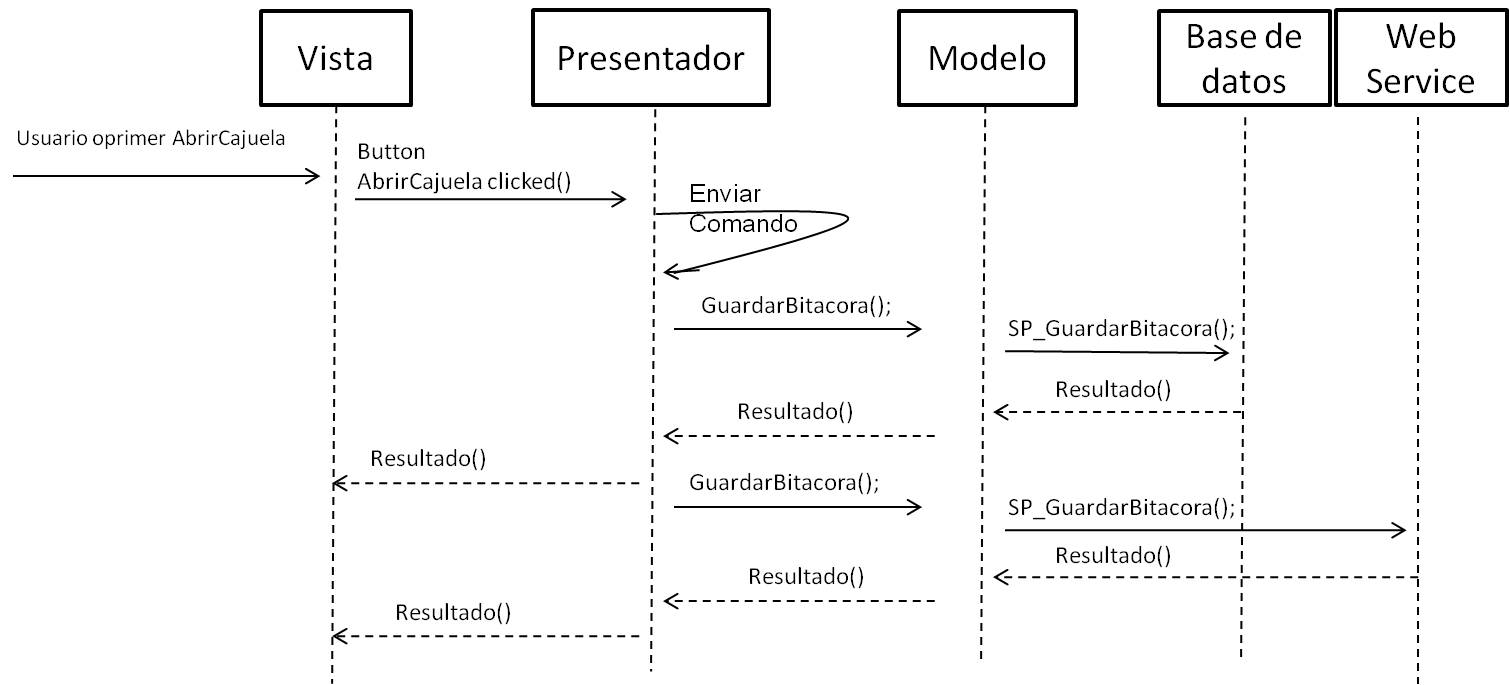
\includegraphics[width=0.95\textwidth]{metodologia/DSAbrirCajuela.jpg}
\caption{Diagrama de secuencia del flujo de la funcionalidad abrir cajuela.}
\label{ds10}
\end{figure}
%
 \begin{enumerate}
\item El usuario selecciona la opción de abrir cajuela.
\item La capa de presentador toma la información de la opción seleccionada y la envia via Bluetooth a la tarjeta electrónica y espera una respuesta de la tarjeta electrónica por el mismo medio de comunicación.
\item Después de adquirir la respuesta envia a la pantalla un mensaje.
\item La capa presentador envia una petición de guardado hacia la base de datos para el registro de las actividades en la aplicación formando un historial, al igual que envia la información de la bitacora hacia el servicio web para crear un registro de la aplicación en linea.
\end{enumerate}

La Figura \ref{ds11} se muestra el evento de la secuencia de poner en modo ignición para el encendido automatico.\\
\begin{figure}[H]
%\vspace{0.2cm}
\centering
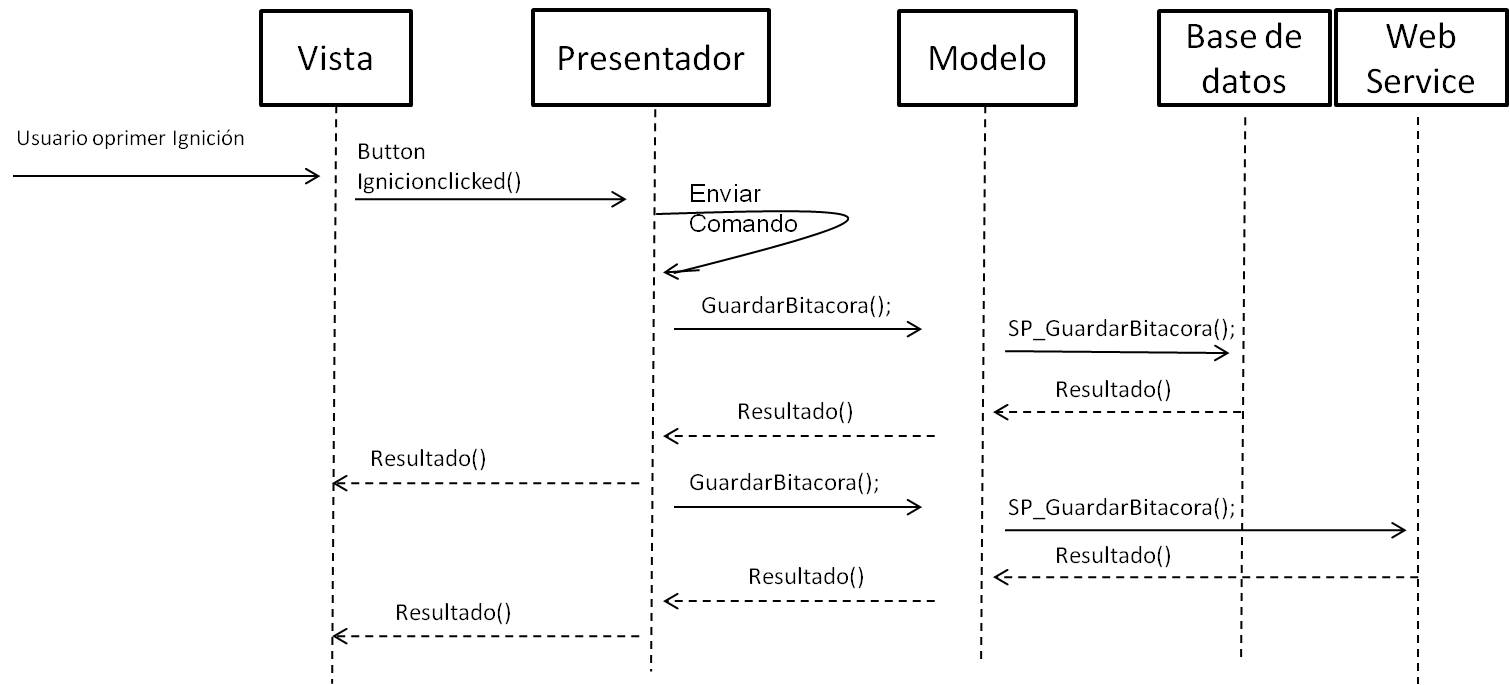
\includegraphics[width=0.95\textwidth]{metodologia/DSIgnicion.jpg}
\caption{Diagrama de secuencia del flujo de la funcionalidad ignición para el encendido automatico.}
\label{ds11}
\end{figure}
%
 \begin{enumerate}
\item El usuario selecciona la opción encendido automatico ignición.
\item La capa de presentador toma la información de la opción seleccionada y la envia via Bluetooth a la tarjeta electrónica y espera una respuesta de la tarjeta electrónica por el mismo medio de comunicación.
\item Después de adquirir la respuesta envia a la pantalla un mensaje.
\item La capa presentador envia una petición de guardado hacia la base de datos para el registro de las actividades en la aplicación formando un historial, al igual que envia la información de la bitacora hacia el servicio web para crear un registro de la aplicación en linea.
\end{enumerate}

La Figura \ref{ds12} se muestra el evento de la secuencia de arrancar la marcha para el encendido automatico.\\
\begin{figure}[H]
%\vspace{0.2cm}
\centering
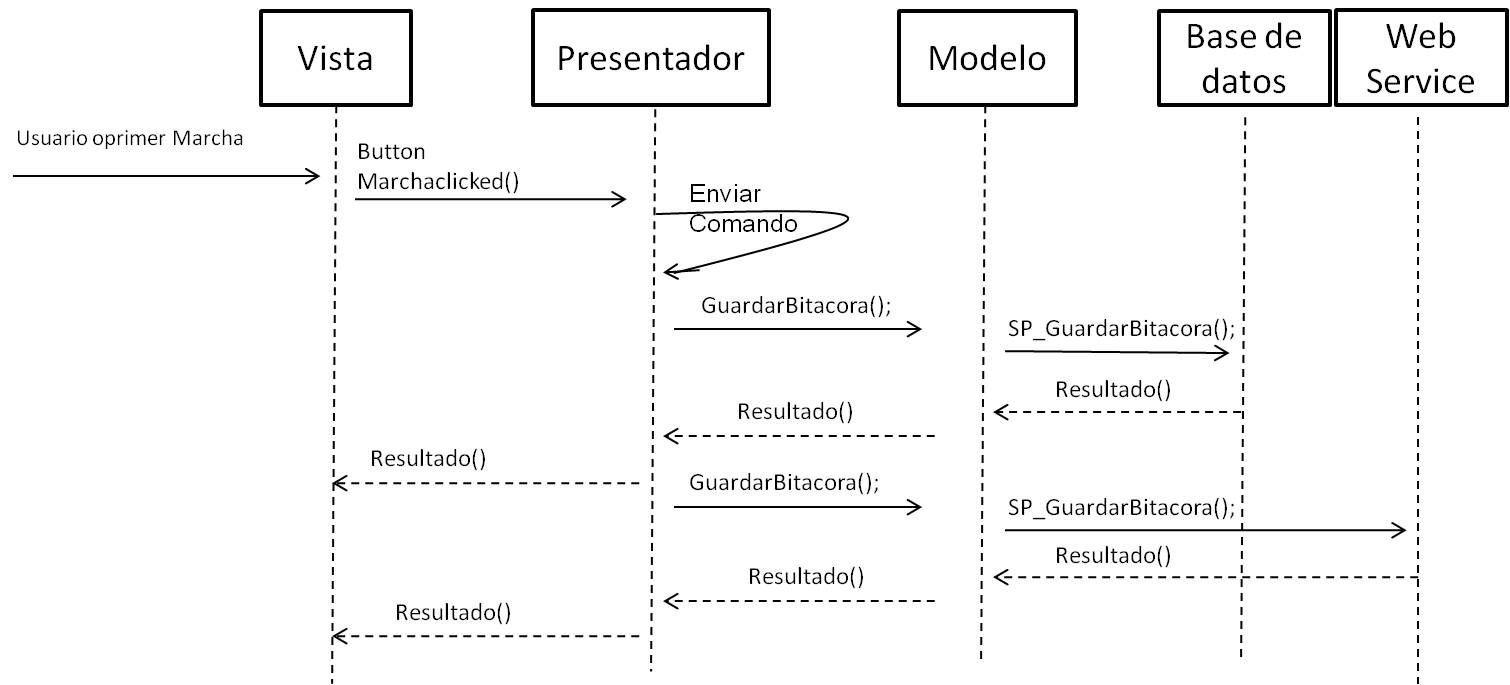
\includegraphics[width=0.95\textwidth]{metodologia/DSMarcha.jpg}
\caption{Diagrama de secuencia del flujo de la funcionalidad marcha para el encendido autoamtico.}
\label{ds12}
\end{figure}
%
 \begin{enumerate}
\item El usuario selecciona la opción encendido automatico marcha.
\item La capa de presentador toma la información de la opción seleccionada y la envia via Bluetooth a la tarjeta electrónica y espera una respuesta de la tarjeta electrónica por el mismo medio de comunicación.
\item Después de adquirir la respuesta envia a la pantalla un mensaje.
\item La capa presentador envia una petición de guardado hacia la base de datos para el registro de las actividades en la aplicación formando un historial, al igual que envia la información de la bitacora hacia el servicio web para crear un registro de la aplicación en linea.
\end{enumerate}

Se realizó una configuración para el envio de información desde el dispositivo móvil con un servicio Web, este servicio nos permitirá conocer las actividades que realiza el usuario, a su vez nos ayudarán a automatizar nuevas funcionalidades y a visualizar las necesidades del usuario según su historial de funcionalidad. El funcionamiento de la comunicación entre la aplicación y el servicio Web de muestra en la Figura \ref{webservice}. Estás bitácoras se visualizan desde el servidor mediante una aplicación Web, tal cual se muestra en la Figura \ref{bitacoraweb}


\begin{figure}[H]
%\vspace{0.2cm}
\centering
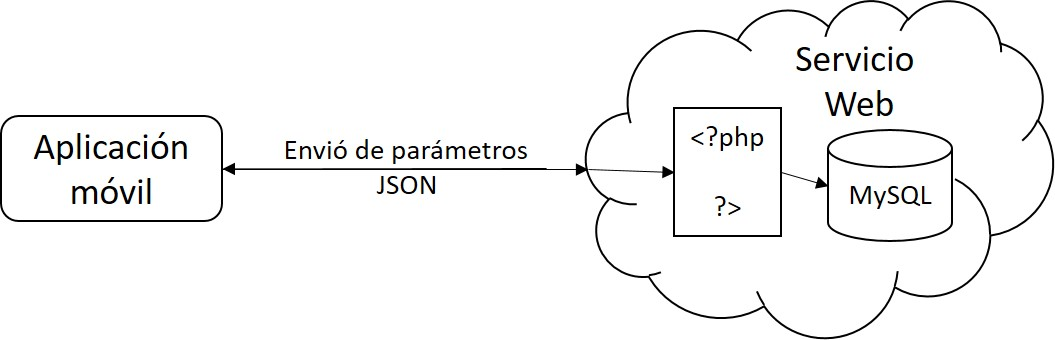
\includegraphics[width=0.95\textwidth]{metodologia/webservice.jpg}
\caption{Comunicación entre la aplicación móvil y el servicio Web.}
\label{webservice}
\end{figure}
%

\begin{figure}[H]
%\vspace{0.2cm}
\centering
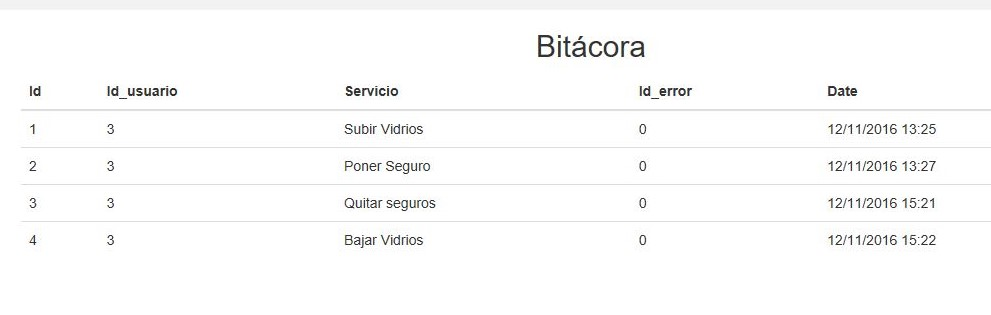
\includegraphics[width=0.95\textwidth]{aplicacion/bitacoraweb.jpg}
\caption{Aplicación para visualizar el historial de los usuarios.}
\label{bitacoraweb}
\end{figure}


El proceso de instalación del archivo .apk se enumera en la siguiente lista: \\
\begin{enumerate}
\item descargar el archivo.
\item acceder a ajustes despúes a Pantalla bloqueo/seguridad.
\item permitir fuentes desconocidas.
\item abrir el archivo descargado.
\item seleccionar la opción instalar.
\item esperar a que se instale.
\item presionar el botón Hecho o abrir.

\end{enumerate}



El funcionamiento de la aplicación móvil es el siguiente. Lo primero que aparece es solicitar el usuario y la contraseña tal como se muestra en la Figura \ref{login1} incisos a, b y c, en donde se pone un bloque de seguridad para evitar accesos no deseados.

\begin{figure}[H]
\centering
\subfigure[]{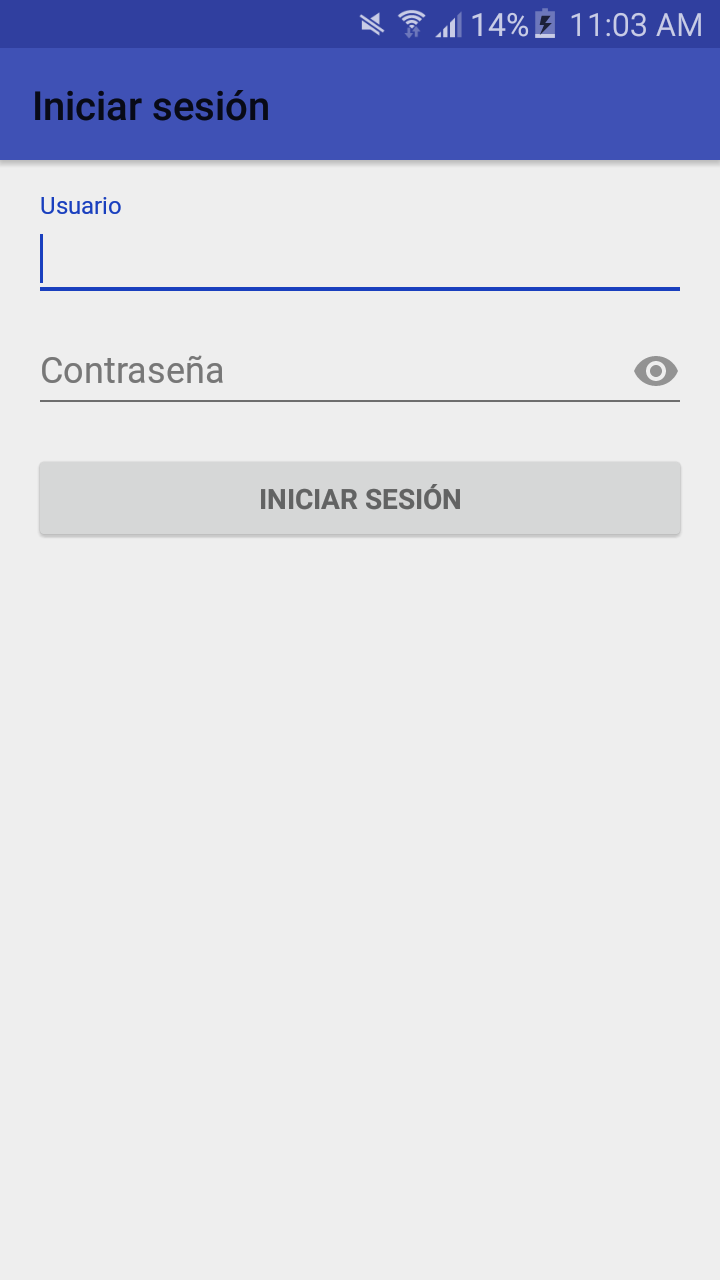
\includegraphics[width=50mm]{aplicacion/login1.jpg}}\hspace{5mm}
\subfigure[]{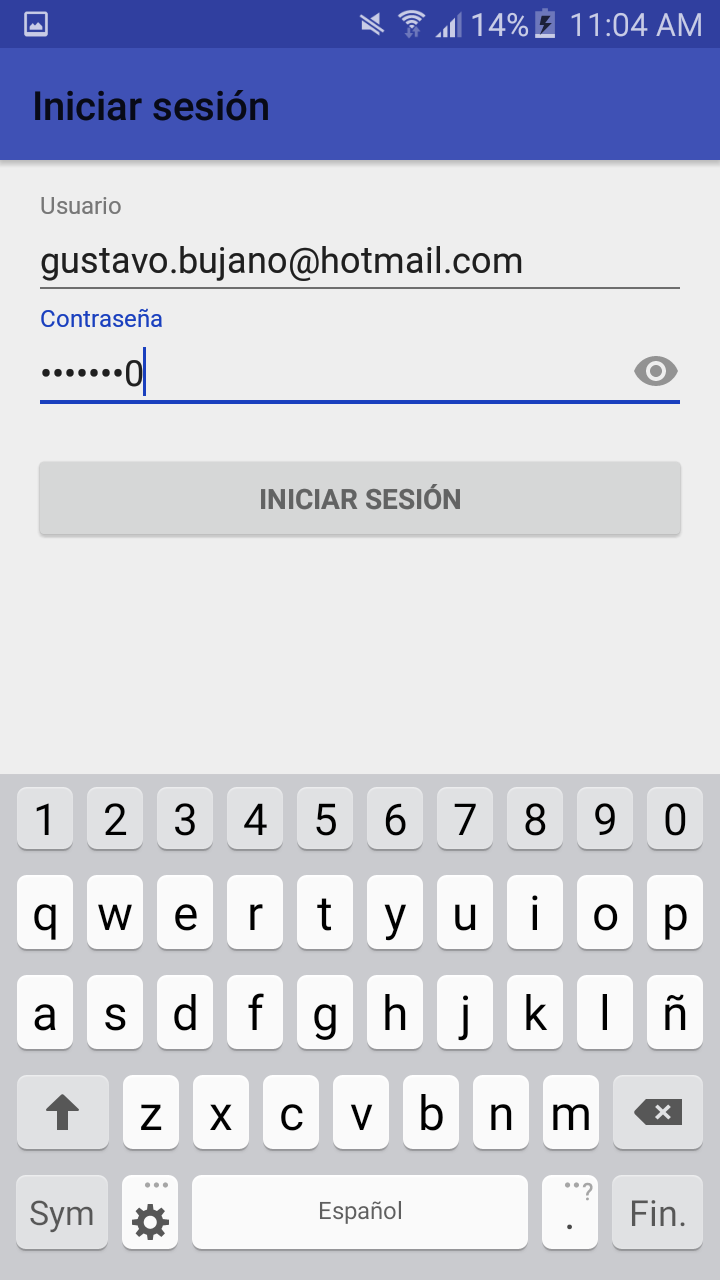
\includegraphics[width=50mm]{aplicacion/login2.jpg}}\hspace{5mm}
\subfigure[]{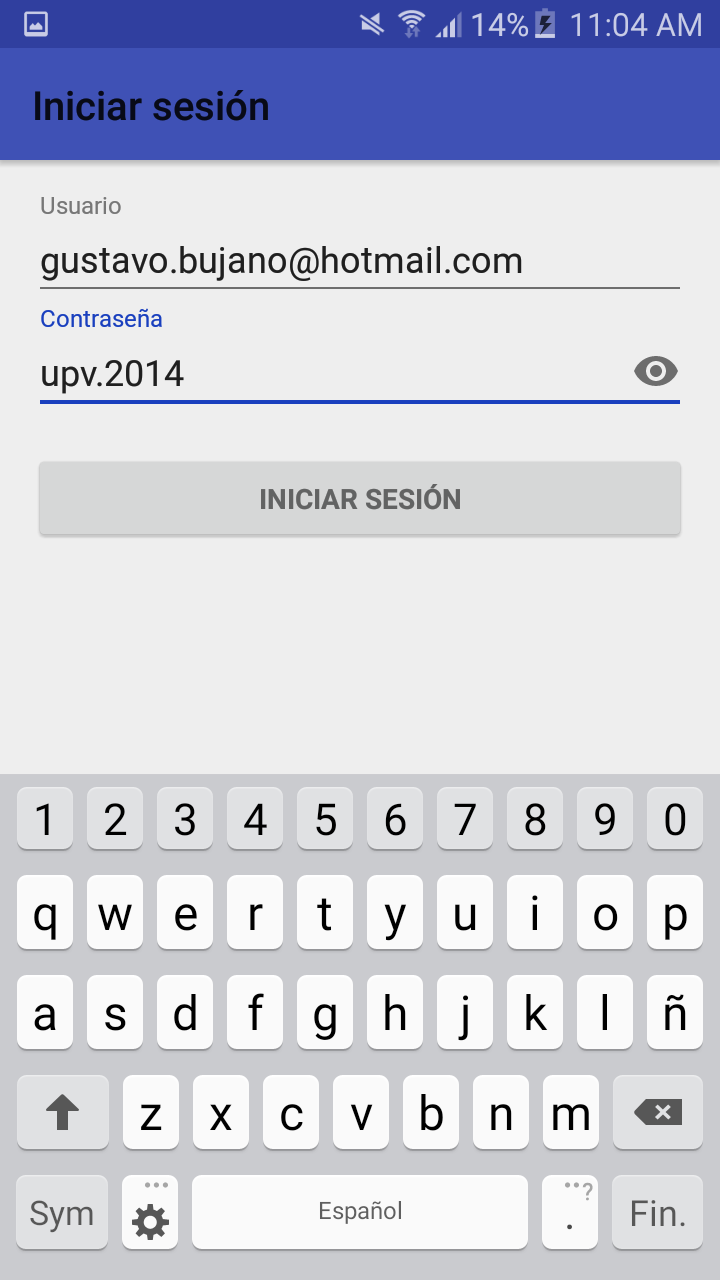
\includegraphics[width=50mm]{aplicacion/login3.jpg}}\hspace{5mm}
\caption{Login de la aplicación.}
\label{login1}
\end{figure}

Una vez ingresado el usuario y la contraseña de manera correcta se mostrará una pantalla principal, en ella se muestra si se encuentra activado el \textit{Bluetooth} ver Figura \ref{principal} inciso a, en caso de no estar activado, la aplicación de manera automática activa el \textit{Bluetooth}, ver Figura \ref{principal} inciso b, y queda a la espera de que el usuario, para desactivar el \textit{Bluetooth} el usuario necesita oprimir el boton con el icono simplemente.\\

\begin{figure}[H]
\centering
\subfigure[]{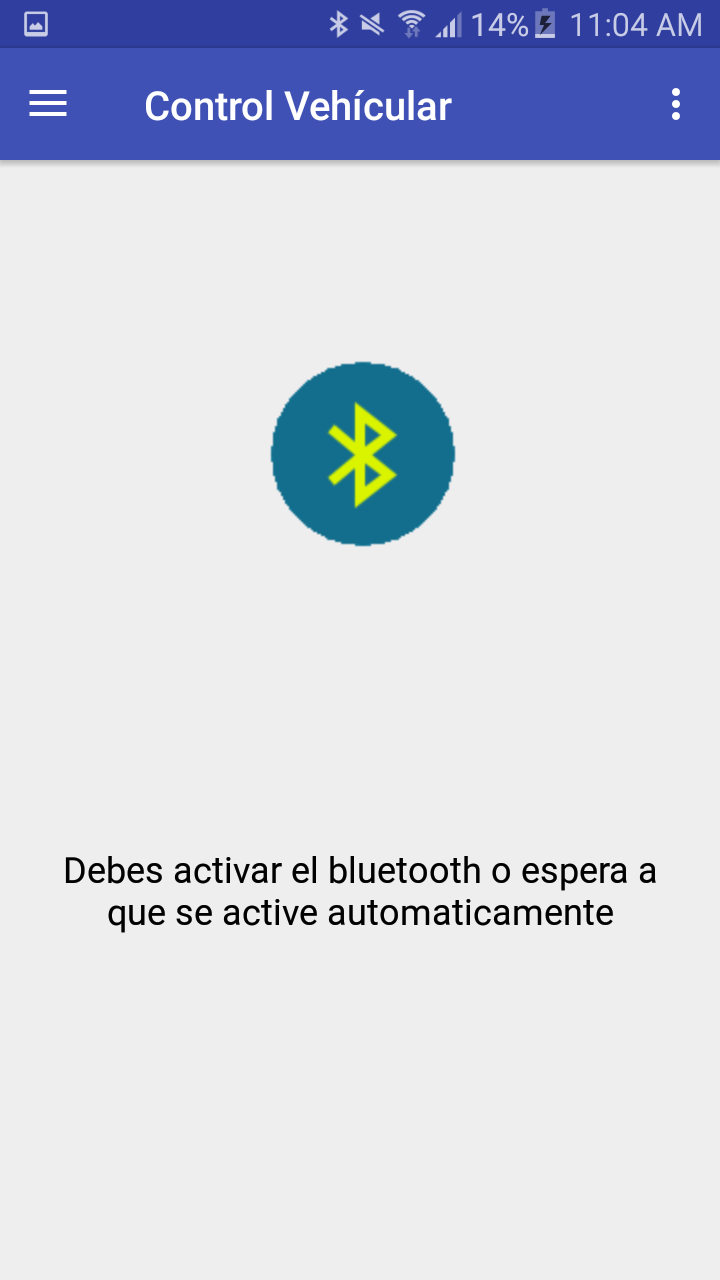
\includegraphics[width=50mm]{aplicacion/principal1.jpg}}\hspace{5mm}
\subfigure[]{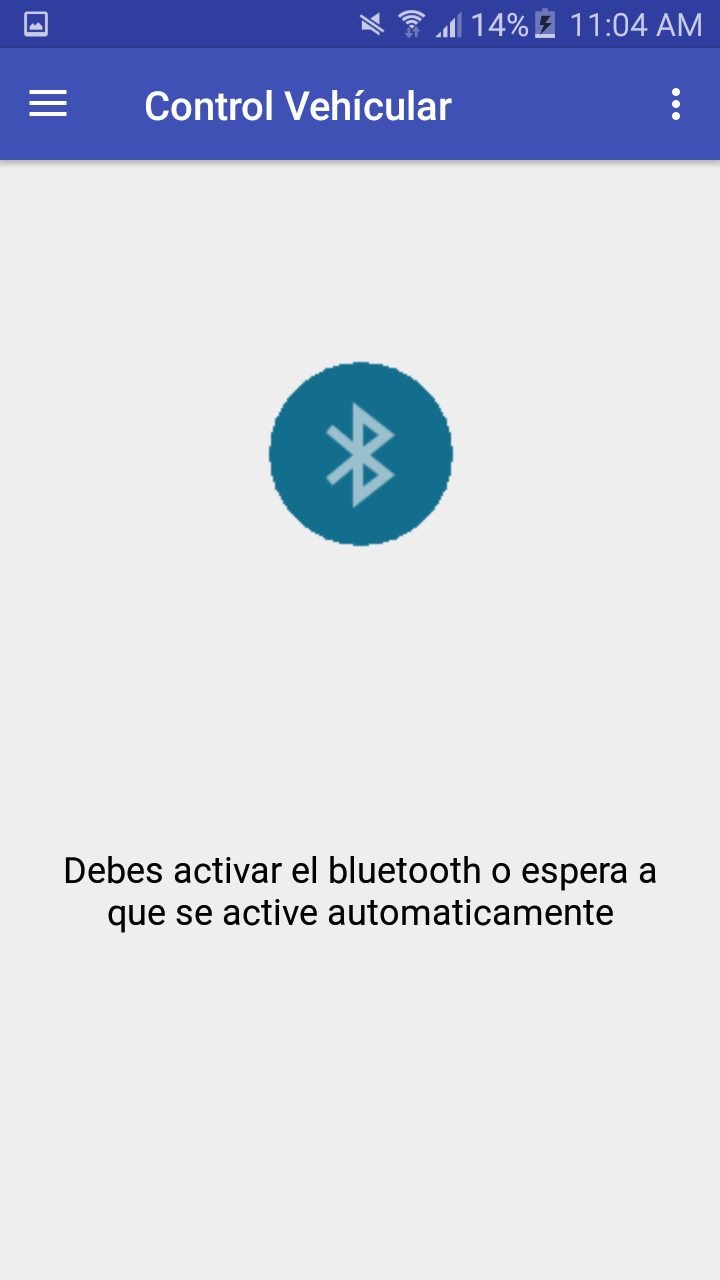
\includegraphics[width=50mm]{aplicacion/principal2.jpg}}\hspace{5mm}
\caption{Pantalla principal de la aplicación.}
\label{principal}
\end{figure}

Dentro de la pantalla principal el sistema cuenta con un menu oculto que se encuentra del lado superior izquierdo, tal cual se muestra en la Figura\ref{menu}. Por otro lado del lado derecho la aplicación cuenta con funcionalidades de preferencia, como: cambiar contraseña, cerrar sesion y ayuda ver Figura \ref{preferencias}.

%
\begin{figure}[H]
%\vspace{0.2cm}
\centering
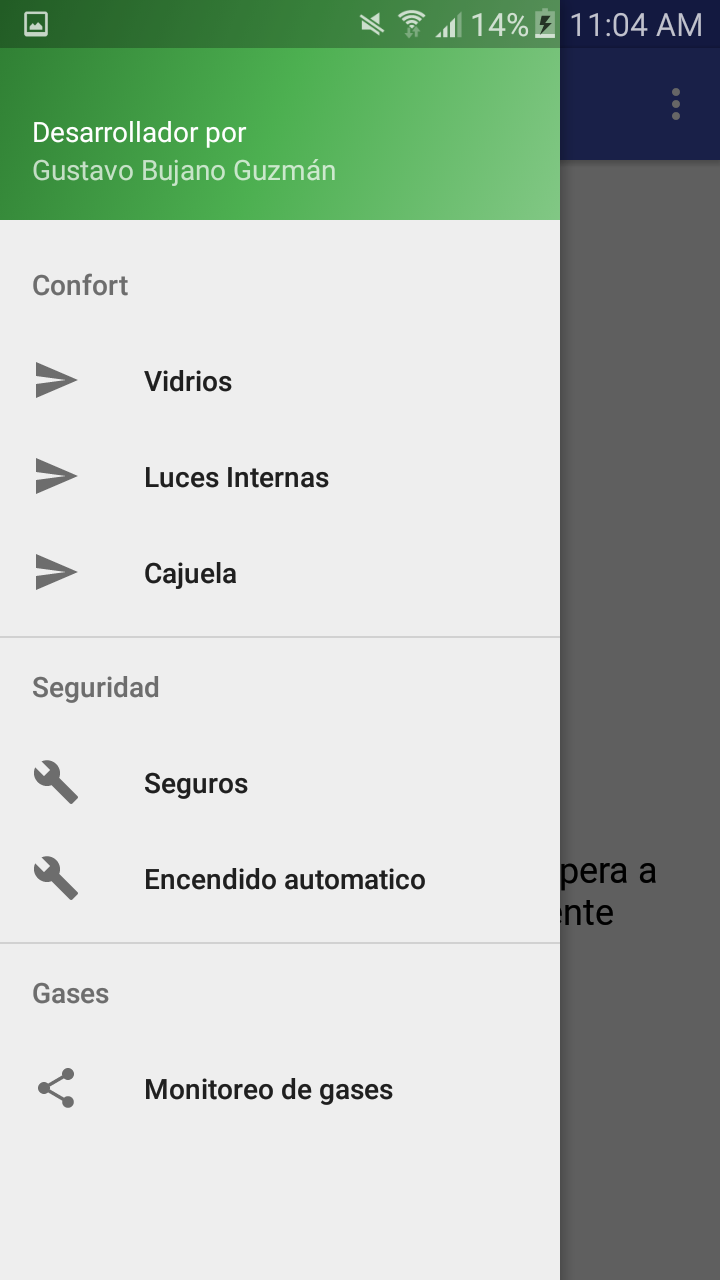
\includegraphics[width=0.4\textwidth]{aplicacion/menu.jpg}
\caption{Menu de opciones de la aplicación.}
\label{menu}
\end{figure}

%
\begin{figure}[H]
%\vspace{0.2cm}
\centering
\includegraphics[width=0.4\textwidth]{aplicacion/preferencias.jpg}
\caption{Menu de preferencias de la aplicación.}
\label{preferencias}
\end{figure}

Dentro del menu, se encuentran todas las funcionalidades hacia el vehículo, englobados  por 4 secciones, a)confort, b)seguridad, c) gases y d) Otros:
 \begin{enumerate}
\item Funcionalidad de vidrios electrícos, Ver Figura \ref{vidrios}. En esta pantalla el usuario puede enviar la señal para bajar el vidrios como se muestra en el incisoa, o subir un vidrio tal cual se muestran en el inciso b.


\begin{figure}[H]
\centering
\subfigure[]{\includegraphics[width=50mm]{aplicacion/vidrios.jpg}}\hspace{5mm}
\subfigure[]{\includegraphics[width=50mm]{aplicacion/vidrios2.jpg}}\hspace{5mm}
\caption{Pantalla del la funcionalidad para los vidrios electrícos.}
\label{vidrios}
\end{figure}

\item Funcionalidad de luces, ver Figura \ref{luces}. En esta pantalla el usuario puede enviar la señal para activar o desactivar las luces, tanto internas ver inciso a, y externas ver inciso b.

\begin{figure}[H]
\centering
\subfigure[]{\includegraphics[width=50mm]{aplicacion/luces.jpg}}\hspace{5mm}
\subfigure[]{\includegraphics[width=50mm]{aplicacion/luces2.jpg}}\hspace{5mm}
\caption{Pantalla del la funcionalidad para las luces.}
\label{luces}
\end{figure}

\item Funcionalidad de cajuela, ver Figura \ref{cajuela}. En esta pantalla el usuario puede enviar la señal para activar el desbloqueo de la cajuela.

\begin{figure}[H]
\centering
\subfigure[]{\includegraphics[width=50mm]{aplicacion/cajuela.jpg}}\hspace{5mm}
\caption{Pantalla del la funcionalidad para la cajuela.}
\label{cajuela}
\end{figure}

\item Funcionalidad de seguros. Ver Figura \ref{seguros}. En esta pantalla el usuario puede enviar la señal para activar o desactivar los seguros de las puertas.

\begin{figure}[H]
\centering
\subfigure[]{\includegraphics[width=50mm]{aplicacion/seguros.jpg}}\hspace{5mm}
\caption{Pantalla del la funcionalidad para los seguros de las puertas.}
\label{seguros}
\end{figure}

\item Funcionalidad de encendido automatico, ver Figura \ref{encendido}. Esta funcionalidad permite activar la ignición y posteriormente se podrá activar la marcha 2 segundos para que el vehículo pueda encender.
\begin{figure}[H]
\centering
\subfigure[]{\includegraphics[width=50mm]{aplicacion/encendido.jpg}}\hspace{5mm}
\subfigure[]{\includegraphics[width=50mm]{aplicacion/encendido2.jpg}}\hspace{5mm}
\caption{Pantalla del la funcionalidad para el encendido automatico.}
\label{encendido}
\end{figure}

\item Funcionalidad de monitoreo de gases, ver Figura \ref{monitoreo}. Esta funcionalidad permite visualizar los niveles de óxido de nitrógeno del vehículo.

\begin{figure}[H]
\centering
\subfigure[]{\includegraphics[width=50mm]{aplicacion/monitore.jpg}}\hspace{5mm}
\caption{Pantalla del la funcionalidad para el monitoreo de óxido de Nitrógeno.}
\label{monitoreo}
\end{figure}

\item Funcionalidad de comandos automáticos, ver Figura  \ref{comandos}. Esta funcionalidad permite ejecutar dos o más comandos en secuencia. En este caso se encuentra un comando automático, poner seguro a las puertas y subir los vidrios.

\begin{figure}[H]
\centering
\subfigure[]{\includegraphics[width=50mm]{aplicacion/comandos.jpg}}\hspace{5mm}
\caption{Pantalla del la funcionalidad para comandos automátizados.}
\label{comandos}
\end{figure}

\item Funcionalidad de Bitácora, ver Figura \ref{bitacora}. Esta funcionalidad permite mostrar todos los comandos que se han ejecutado en la aplicación.
\begin{figure}[H]
\centering
\subfigure[]{\includegraphics[width=50mm]{aplicacion/bitacora.jpg}}\hspace{5mm}
\caption{Pantalla del la funcionalidad bitácora.}
\label{bitacora}
\end{figure}

\end{enumerate}











\subsection{CONECTIVIDAD}

Bluetooth es la tecnología que se ha seleccionado para realizar la conectividad debido a su tendencia en la comunicación inalámbrica y su compatibilidad. Actualmente los dispositivos móviles ya cuentan con esta tecnología. Por otra parte, se le ha conectado a la tarjeta electrónica el \textit{shield} Bluetooth HC-05 tal cual se muestra en las Figuras \ref{conexion} y \ref{conexion2}\\


%
\begin{figure}[H]
%\vspace{0.2cm}
\centering
\includegraphics[width=0.8\textwidth]{metodologia/conexion_bluetooth2.jpg}
\caption{Simulación de la conexión de la tarjeta electrónica y el \textit{shild} Bluetooth}
\label{conexion2}
\end{figure}

%
\begin{figure}[H]
%\vspace{0.2cm}
\centering
\includegraphics[width=0.8\textwidth]{metodologia/conexion_bluetooth.jpg}
\caption{Conexión de la tarjeta electrónica y el \textit{shild} Bluetooth}
\label{conexion}
\end{figure}


El proceso de conexión entre el disositivo móvil y la tarjeta electrónica por primera vez se muestra a continuación:

\begin{enumerate}
\item Activar la tarjeta electrónica para que se active el shield bluetooth.
\item Activar el bluetooth del dispositivo móvil.
\item Acceder a la configuración del bluetooth del disposito.
\item Seleccionar en dispositivo disponible el preferido (ver Figura \ref{vinc} inciso a).
\item Introducir el PIN para vincular el dispositivo (ver Figura \ref{vinc} inciso b).
\item El dispositivo se mostrará vinculado (ver Figura \ref{vinc} inciso c).
\end{enumerate}

\begin{figure}[H]
\centering
\subfigure[]{\includegraphics[width=50mm]{metodologia/vinc.png}}\hspace{5mm}
\subfigure[]{\includegraphics[width=50mm]{metodologia/vinc1.png}}\hspace{5mm}
\subfigure[]{\includegraphics[width=50mm]{metodologia/vinc2.png}}
\caption{Proceso de conexión de bluetooth en el dispositivo móvil.} \label{vinc}
\end{figure}

Una vez finalizado este proceso, la comunicación se realiza con la tarjeta electrónica mediante la aplicación móvil.

\subsection{TARJETA ELECTRÓNICA}

La tarjeta electrónica que se utilizó fue Arduino utilizando el microcontrolador ATMega 3282P, esta se conecta por medio del bluetooth hacia el celular para recibir las variables enviadas.\\



\subsection{CIRCUITO DE POTENCIA}

El circuito de potencia que se elaboró se repite N veces según sean las señales enviadas por parte de la tarjeta electrónica. Este circuito se encarga de recibir la señal de la tarjeta electrónica y activar o desactivar un relevador. Este relevador a su vez permite o denegar el acceso de la señal \textit{low} y así accionar o detener el actuador. El circuito esta conformado por la señal que accede desde la tarjeta electrónica, un capacitor, un transistor y una resistencia armados tal como se muestra en la Figura \ref{circuito_potencia}.  \\

%
%\begin{figure}[H]
%\vspace{0.2cm}
%\centering
%\includegraphics[width=0.8\textwidth]{metodologia/nodisponible.jpg}
%\caption{circuito de potencia hechizo}
%\label{circuito_potencia}
%\end{figure}

\subsection{ACTUADORES Y SENSORES}

   
\paragraph{Sensor de gas MQ-135}
 (ver Figura \ref{sensor}) sirve para medir el óxido de nitrógeno entre otras cosas, este se coloca dentro del vehículo para medir las emisiones que salen referente al óxido de nitrógeno.\\

%
\begin{figure}[H]
%\vspace{0.2cm}
\centering
\includegraphics[width=0.5\textwidth]{metodologia/fig_sensor.jpg}
\caption{Conexión del sensor y la tarjeta programable. }
\label{sensor}
\end{figure}
%

La tarjeta del sensor cuenta con dos salidas de datos, una digital (DO) y otra analógica (AO) (ver Figura \ref{descripcion_sensor}). La salida digital manda una señal en estado alto cuando el sensor llega a un nivel deseado, el cual puede ser ajustado por medio del potenciómetro. La salida analógica va aumentado el valor del voltaje en proporción al nivel de gas que se detecta.\\

%
\begin{figure}[H]
%\vspace{0.2cm}
\centering
\includegraphics[width=0.5\textwidth]{metodologia/gas_4.png}
\caption{Descripción de las salidas del sensor. }
\label{descripcion_sensor}
\end{figure}
%

Este sensor se conecta directamente a la tarjeta programable, la conexión se muestra en la Figura \ref{conexion_sensor}, para obtener los datos en partes por millón (ppm) es necesario hacer la conversión con el programa que se encuentra en el anexo 1.
%
\begin{figure}[H]
%\vspace{0.2cm}
\centering
\includegraphics[width=0.5\textwidth]{metodologia/gas_5.png}
\caption{Conexión del sensor y la tarjeta programable. }
\label{conexion_sensor}
\end{figure}
%

la Configuración del puerto serial sirve para cargar el programa e ingresar al monitor serial que ofrece el Arduino es necesario asegurarse que el puerto COM sea el correcto.  Para ello tenemos que acceder a “Administrador de dispositivos” (ver Figura \ref{conf_puerto} desde la PC y verificar que el COM que nos muestra sea el mismo que marca el \textit{software} de Arduino.

\begin{figure}[H]
%\vspace{0.2cm}
\centering
\includegraphics[width=0.5\textwidth]{metodologia/gas_6.png}
\caption{Configurando el puerto serial. }
\label{conf_puerto}
\end{figure}
%

En caso de que no coincida el puerto COM entre el “Administrador de dispositivos” y el marcado en el \textit{software} podemos cambiarlo en la barra de herramientas (ver Figura \ref{conf_puerto2}).

\begin{figure}[H]
%\vspace{0.2cm}
\centering
\includegraphics[width=0.5\textwidth]{metodologia/gas_7.png}
\caption{Configurando el puerto desde la barra de herramientas. }
\label{conf_puerto2}
\end{figure}


Una vez que este verificado el puerto serial soló damos clic en la lupa que aparece en la parte superior derecha y automáticamente abre otra ventana que muestra el puerto serial (ver Figura \ref{conf_puerto22}.

\begin{figure}[H]
%\vspace{0.2cm}
\centering
\includegraphics[width=0.5\textwidth]{metodologia/gas_8.png}
\caption{ventana para visualizar la información. }
\label{conf_puerto22}
\end{figure}

\paragraph{Actuador Vidrios Eléctricos} es un mecanismo con un motor electríco incluido de fábrica en algunos vehículos, el auto de prueba maneja un sistema completamente mecánico y a través de una manija eleva o bajar el vidrio.\\

Los pasos que se desarrollaron para automatizar este actuador fueron los siguientes.\\

\begin{enumerate}
\item verificar que las gomas estuvieran en buenas condiciones para evitar que el agua se filtrará dentro de la puerta.\\
\item implementar el motor del elevador de vidrio al sistema mecánico, en esta parse se tuvo la necesidad de adaptar el motor con el sistema de elevación, generando unas ranuras para incluir pernos y así evitar que la fuerza del motor destruyera el sistema de elevación.\\
\item instalar y probar directamente en el acumulador tal cual se muestra en la Figura \ref{subirvidrio}, se implementó un control manual para manipular la actividad de subir y bajar el vidrio. Los diagramas que se ocuparón para el control manual se muestran en la Figura \ref{control_manual}.

\end{enumerate}





\begin{figure}[H]
%\vspace{0.2cm}
\centering
\includegraphics[width=0.7\textwidth]{metodologia/subirvidrio.jpg}
\caption{Instalación del motor en la puerta}
\label{subirvidrio}
\end{figure}

\begin{figure}[H]
%\vspace{0.2cm}
\centering
\includegraphics[width=0.7\textwidth]{metodologia/diagramacontrol.png}
\caption{Configuración del control Manual}
\label{control_manual}
\end{figure}

Al final se realizó un circuito generando un puente H para subir y bajar el vidrio con el dispositivo móvil tal cual se muestra en la Figura \ref{circuito_android}, evitando que las señales colisionen entre el control manual y el dispositivo móvil.

%
\begin{figure}[H]
%\vspace{0.2cm}
\centering
\includegraphics[width=0.8\textwidth]{metodologia/nodisponible.jpg}
\caption{XXXX}
\label{circuito_android}
\end{figure}


\paragraph{Actuador Seguros de Puertas}
es un sistema que se le adapta al vehículo para que la puerta no se pueda abrir, evitando accidentes cuando el vehículo se encuentre en movimiento,principalmente.\\

Lo primero que se realizó en esta actividad fue incorporar los seguros e instalarlos dentro de las puertas tal cual se muestra en la Figura \ref{seguros}.
%%
%\begin{figure}[H]
%\vspace{0.2cm}
%\centering
%\includegraphics[width=0.8\textwidth]{metodologia/nodisponible.jpg}
%\caption{XXXX}
%\label{seguros}
%\end{figure}

Una vez instalados se probaron directamente con la batería de vehículo, y se realizó un circuito generando un puente H para subir y bajar el seguro con el dispositivo móvil tal cual se muestra en la Figura\ref{abrir_cerrar_seguros}.
%
%\begin{figure}[H]
%\vspace{0.2cm}
%\centering
%\includegraphics[width=0.8\textwidth]{metodologia/nodisponible.jpg}
%\caption{XXXX}
%\label{abrir_cerrar_seguros}
%\end{figure}


\paragraph{Sistema de Ignición y Marcha}




\paragraph{Actuador Luces Interiores y Exteriores}
un sistema de iluminación interno, normalmente aparece cuando abrimos una puerta o mediante un botón de iluminación. Un sistema de iluminación externo es cuando accionamos un boton para que las luces delanteras se iluminen. 

Lo primero que hicimos fue realizar la estructura y se visualizó la forma de encender mediante el dispositivo móvil las luces, tanto interiores como exteriores.

Luego se realizo el circuito electríco tal cual se muestra en la Figura \ref{luces}, tanto el sistema interno como el externo trabajan de la mismo forma.
%
%\begin{figure}[H]
%\vspace{0.2cm}
%\centering
%\includegraphics[width=0.8\textwidth]{metodologia/nodisponible.jpg}
%\caption{XXXX}
%\label{luces}
%\end{figure}


\paragraph{Actuador Cajuela}
la cajuela es un apartado que tiene el vehículo que permite introducir objetos en él.
para que la cajuela se habrá de manera automática mediante el dispositivo móvil depende de dos actividades, el abrir la cerradura y el levantamiento de la cajuela.
para el abrir la cerradura debe de existir un motor que jale la varilla que hace la función de abrir la cerradura, por la cuestión del levantamiento de la cajuela se cambiaron los pistones, los cuales una vez abierta la cerradura hacen su función de manera inmediata.


\clearpage
\section{Análisis de los Resultados}

En esta sección se mostrarán los resultados detallados que se obtuvieron durante las pruebas realizadas en este proyecto. Los resultados son plasmados por actividades realizadas para una mayor compresión.\\

\subsection {Resultado del trabajo previo}

Los resultados preliminares que se han obtenido son el funcionamiento correcto de la red Can Bus, además de la verificación del conector de enlace de datos en conjunto con el protocolo de comunicación J1850 VPW, el cual indica la combinación de pines, sin embargo, el escáner EML327 con el cual se trabajó solamente puede detectar información sobre el Sistema de Tracción, debido a que la mayoría de los vehículos cuentan con características muy parecidas en el sistema de tracción, sin embargo, el sistema de confort depende de cada vehículo.\\

El sistema de confort del vehículo Sentra 2006 XLS es un sistema descentralizado lo cual indica que existen diferentes módulos para el sistema de confort, cada módulo se encarga de actividades en específico. Por lo cual seguir con esta linea de investigación requeriria de muchos recursos no disponibles al momento, es por esto que se optó por reajustar la linea de investigación a otro tipo de vehículos.



\subsection {Aplicación móvil}

Se realizaron pruebas de comunicación entre la aplicación móvil y la tarjeta programable, la conexión se encuentra estable durante todo el proceso, sin embargo, tiene un límite de distancia para enviar y recibir los paquetes no mayor a 10 metros, después de dicha distancia la aplicación envía un mensaje de error de conexión.\\

Durante su funcionamiento en caso de ser cerrada la aplicación de forma inesperada conlleva a tener errores de comunicación la siguiente vez que se desea conectar debido a que el dispositivo bluetooth se queda con la conexión anterior, así que se tiene que esperar un par de minutos para que el dispositivo funcione de manera correcta.\\

La arquitectura Modelo Vista Presentador permite modificar de una manera sencilla la aplicación en temas de interfaces para el usuario, reglas de negocio o conexiones a base de datos.

Parte de la aplicación esta enfocada a recolectar datos en forma de un historial, este historial tiene la finalidad de crear patrones de usabilidad en la aplicación permitiendo generar comandos automaticos para mejorar la experiencia del usuario.

La aplicación cuenta con una base de datos local para el acceso sin la necesidad de conexión a internet, aunque cuando se tiene acceso envia las bitacoras de actividades a un servicio web que almacena la información en una base de datos remota, con la finalidad de proponer comandos automatizados para mejorar la aplicación y detectar patrones de los usuarios.

\subsection{Comunicación}

Las pruebas que se realizaron de comunicación han sido exitosas cuando el dispositivo móvil está a menos de 10 metros de la tarjeta programable, este tipo de comunicación permite la conexión punto a punto, lo cual evita que más de un dispositivo móvil se conecte y así evitar ordenes no deseadas.\\

En caso de que exista algún bloqueo o falla en la comunicación por los diferentes factores posibles, la tarjeta electrónica tiene un botón de reinicio, en donde permite que la comunicación se vuelva a iniciar de manera normal.\\

La comunicación es bidireccional debido a que el dispositivo móvil envía los datos hacia la tarjeta programable, y la tarjeta programable envia una respuesta, sin embargo, la tarjeta electrónica es unidireccional hacia los actuadores debido a que no verifica fisicamente la actividad, unicamente envia las señal a los relevadores, pero estos no responen a la tarjeta electrónica, por lo cual en caso de un fallo con algun actuador o relevador la tarjeta electrónica no puede detectar este detalle. No obstante el caso con el sensor de oxido de nitrogeno es un apartado diferente, debido a que la comunicación con el sensor si es bidireccional.\\

\subsection{Tarjeta electrónica}

Se realizaron pruebas de comunicación recibiendo las variables del dispositivo móvil, estas resultaron de manera correcta la tarjeta programable recibe la comunicación e interpreta los parámetros, después activa los pines según sea la condición seleccionada.\\

Parte de las actividades que no realiza la tarjeta electrónica es la comprobación del funcionamiento, cuando existe un problema con algun actuador el sistema no reconoce la falla automaticamente.

\subsection{Circuito de potencia}

El circuito de potencia que se realizó permite activar o desactivar el relevador de manera correcta, este circuito se realizó N veces dependiendo de los diferentes actuadores que se manipularon. Sin embargo, tiene la misma problematica que la tarjeta electrónica y el medio de comunicación, carece de una verificación fisica del funcionamiento del actuador.\\

\subsection{Actuadores y sensores}

Para analizar el comportamiento del sensor se colocó dentro de un mofle y se encendió el vehículo para que emitiera los gases por el mofle y con la ayuda del puerto serial se pudo observar los datos obtenidos del sensor.

Por parte de los actuadores, se instalaron debidamente en el vehículo, sin embargo los actuadores no envian señales de respuesta, por lo cual en caso de una falla no existe un sensor que auxilie al usuario mencionandole el problema.






\clearpage
\section{Conclusión}

En conclusión, podemos mencionar que aumentar la seguridad y confort en un vehículo de gama baja es un trabajo con grandes intereses. El conocer el nivel del óxido de nitrógeno que emite el vehículo también es un parámetro interesante para enviar el automóvil a revisión y contribuir al medio ambiente\\

Este proyecto se puede llevar a cabo sin problemas con vehículos de años no recientes, actualmente existen carros nuevos que no tienen ciertos actuadores que se muestran en este proyecto. Sin embargo, no se recomienda instarlos dentro de un vehículo en un tiempo menor a cinco años del modelo del carro debido a que puede tener problemas en el tema de garantía. Las agencias automotrices permiten el mantenimiento preventivo y correctivo los primeros cinco años, después no desean dar mantenimiento a los vehículos debido al tiempo del auto.\\

Durante la elaboración del proyecto se ha llegado a comprender de mejor manera el funcionamiento del vehículo, en específico la parte eléctrica o electrónica, según sea el caso.\\

Durante el trabajo previo se llevo la tarea de provar la funcionalidad del Scanner EML327 y se llego a la conclusión que, aunque muestra información sobre la velocidad, RPM, entre otros. No permite la manipulación de la información de los sensores o de los actuadores y los datos arrojados son pertenecientes al sistema de tracción.\\

Las herramientas y accesorios que se utilizaron para este proyecto son fáciles de encontrar y no se necesitan lugares especializados para comprar. \\
En la mayoría de las actividades que se probaron es conveniente su funcionamiento, a excepción del encendido automático debido a factores que pueden influir negativamente en la seguridad y confort del vehículo, como es el caso de que la marcha se llegue a quemar o que la pila sea descargada por dejar el modo de ignición encendido.\\

Un apartado muy importante es el historial de la aplicación, debido a que registra el patrón de servicios que utiliza el usuario en la aplicación, con una muestra de datos convicente se pueden crear nuevos comandos automatizados.\\

Algunos casos que se proponen son:\\
\begin{enumerate}
\item Al apagar el vehìculo desactivar los seguros.
\item Al activar los seguros subir los vidrios.
\item Al desactivar los seguros bajar los vidrios.
\item Encender las luces exteriores a cierta hora si el vehículo esta encendido.
\end{enumerate}

Cabe mencionar que algunos de los casos que se proponen existen en vehículos modernos, sin embargo, se deben instalar de acuerdo al usuario. ya que existen usuarios por ejemplo, que no bajan los vidrios debido a que encienden el aire acondicionado, entre otros ejemplos.\\

Como trabajo a futuro se puede analizar los datos y proponer nuevos casos de automtización, además de mejorar la aplicación y agregarle nuevas funcionalidades, también es recomendable desarrollar un sistema de comunicación bidireccional entre los actuadores, de tal forma que el usuario pueda estar enterado en caso de un error con algun actuador.



\clearpage
\input{Capitulo6.tex}

\clearpage
\addcontentsline{toc}{section}{Índice de figuras}
\renewcommand\listfigurename{Índice de figuras}
\listoffigures

\clearpage
\addcontentsline{toc}{section}{Índice de cuadros}
\renewcommand\listtablename{Índice de cuadros}
\listoftables

%-----------------------------------------------------------------------------------------------------------------
% REFERENCIAS


\clearpage
%Let's cite! The Einstein's journal paper \cite{dirac} and the Dirac's 
%book \cite{einstein} are physics related items. 

\addcontentsline{toc}{section}{Referencias} 
\printbibliography
% \bibliographystyle{ieeetr}
%\bibliography{Bibliografia}
%\section{Anexo 1}
\subsection{Codigo para obtener los datos del Óxido de Nitrógeno}
Obtención de los datos en partes por millón (ppm) del sensor de gas óxido de nitrógeno.

\begin{verbatim}

//define la entrada analogica para el sensor
#define MQ1 (0) 
//define el valor de la resistencia mde carga en kilo ohms
#define RL_VALOR (5)     
// resistencia del sensor en el aire limpio / RO,
// que se deriva de  la tabla de la hoja de datos
#define RAL (9.83) 
#define GAS_LP  (0)
//Cadena recibida desde el PC
String inputstring = "";                                                        
float           LPCurve[3]  =  {2.3,0.21,-0.47};
float           Ro           =  10;
void setup(){
//Inicializa Serial a 9600 baudios
Serial.begin(9600);                                                                  
 Serial.println("Iniciando ...");
   //configuracion del sensor
  Serial.print("Calibrando...\n");
  //Calibrando el sensor. Por favor de asegurarse que el sensor se encuentre
  // en una zona de aire limpio mientras se calibra
  Ro = Calibracion(MQ1);          
  Serial.print("Calibracion finalizada...\n");
  Serial.print("Ro=");
  Serial.print(Ro);
  Serial.print("kohm");
  Serial.print("\n");
}
 
void loop()
{
   Serial.print("LP:");
   Serial.print(porcentaje_gas(lecturaMQ(MQ1)/Ro,GAS_LP) );
   Serial.print( "ppm" );
   Serial.print("    ");
   Serial.print("\n");
   delay(200);
}
 
float calc_res(int raw_adc)
{
  return ( ((float)RL_VALOR*(1023-raw_adc)/raw_adc));
}
 
float Calibracion(float mq_pin){
  int i;
  float val=0;
    //tomar múltiples muestras
    for (i=0;i<50;i++) {                                                                               
    val += calc_res(analogRead(mq_pin));
    delay(500);
  }
  //calcular el valor medio
  val = val/50;                                                                                         
  val = val/RAL;
  return val;
}
 
float lecturaMQ(int mq_pin){
  int i;
  float rs=0;
  for (i=0;i<5;i++) {
    rs += calc_res(analogRead(mq_pin));
    delay(50);
  }
rs = rs/5;
return rs;
}
 
int porcentaje_gas(float rs_ro_ratio, int gas_id){
   if ( gas_id == GAS_LP ) {
     return porcentaje_gas(rs_ro_ratio,LPCurve);
   }
  return 0;
}
 
int porcentaje_gas(float rs_ro_ratio, float *pcurve){
  return (pow(10, (((log(rs_ro_ratio)-pcurve[1])/pcurve[2]) + pcurve[0])));
}
\end{verbatim}



\end{document}